%%%%%%%%%%%%%%%%%%%%%%%%%%%%%%%%%%%%%%%%%%%%%%%%%%%%%%%%%%%%%%%%%%%%%%
% LaTeX Example: Project Report
%
% Source: http://www.howtotex.com
%
% Feel free to distribute this example, but please keep the referral
% to howtotex.com
% Date: March 2011
%
%%%%%%%%%%%%%%%%%%%%%%%%%%%%%%%%%%%%%%%%%%%%%%%%%%%%%%%%%%%%%%%%%%%%%%
% How to use writeLaTeX:
%
% You edit the source code here on the left, and the preview on the
% right shows you the result within a few seconds.
%
% Bookmark this page and share the URL with your co-authors. They can
% edit at the same time!
%
% You can upload figures, bibliographies, custom classes and
% styles using the files menu.
%
% If you're new to LaTeX, the wikibook is a great place to start:
% http://en.wikibooks.org/wiki/LaTeX
%
%%%%%%%%%%%%%%%%%%%%%%%%%%%%%%%%%%%%%%%%%%%%%%%%%%%%%%%%%%%%%%%%%%%%%%
% Edit the title below to update the display in My Documents
%\title{Project Report}
%
%%% Preamble
\documentclass[paper=a4, fontsize=11pt]{book}
\usepackage[T1]{fontenc}
\usepackage{lmodern}
%\usepackage{fourier}

\usepackage[english]{babel}															% English language/hyphenation
\usepackage[protrusion=true,expansion=true]{microtype}
\usepackage{amsmath,amsfonts,amsthm} % Math packages
\usepackage[pdftex]{graphicx}
\usepackage{url}
\usepackage{caption}
\usepackage[top=0.8in, bottom=0.8in, left=0.8in, right=0.8in]{geometry}
\usepackage{subcaption}  % For placing two subfigures side by side

%%% Custom sectioning
\usepackage{sectsty}
\usepackage{multirow}
\allsectionsfont{\centering \normalfont\scshape}

%%% Inserting landscape pages
\usepackage{pdflscape}
\usepackage{wrapfig}


%%% Custom headers/footers (fancyhdr package)
\usepackage{fancyhdr}
\pagestyle{fancyplain}
\fancyhead{}											% No page header
\fancyfoot[L]{}											% Empty
\fancyfoot[C]{}											% Empty
\fancyfoot[R]{\thepage}									% Pagenumbering
\renewcommand{\headrulewidth}{0pt}			% Remove header underlines
\renewcommand{\footrulewidth}{0pt}				% Remove footer underlines
\setlength{\headheight}{13.6pt}
\setlength{\fboxrule}{1mm}
\setlength{\fboxsep}{5mm}

%%% Equation and float numbering
\numberwithin{equation}{section}		% Equationnumbering: section.eq#
\numberwithin{figure}{section}			% Figurenumbering: section.fig#
\numberwithin{table}{section}				% Tablenumbering: section.tab#


%%% Maketitle metadata
\newcommand{\horrule}[1]{\rule{\linewidth}{#1}} 	% Horizontal rule

\title{
		%\vspace{-1in}
		\usefont{OT1}{bch}{b}{n}
		\horrule{0.5pt} \\[0.2cm]
		\LARGE Integrals of bsplines of degree 0,1,2 and 3\\
        -\\
        \normalsize Another tool for ToFu
		\horrule{2pt} \\[0.3cm]
}
\author{D. VEZINET}
\date{\today}

% Graphics path
\graphicspath{ {./} }

%%% Begin document
\begin{document}
\maketitle

\tableofcontents

\newpage
\section{Introduction}

\subsection{General problem}

Quadrature\footnote{see https://en.wikipedia.org/wiki/Gaussian\_quadrature} is numerical integration by summing the weighted values of the integrand assessed at well-chosen fixed points $\int_a^b f(x)dx = \sum_{i=1}^n w_if(x_i)$.
The points are found by computing the roots of a set of special orthogonal polynomials.\\

Gaussian quadrature is a method of choosing $n$ points and weights such that the result is exact for a polynomial of degree $d \leq 2n-1$.
Hence, for a bspline of degree $d$, the gaussian quadrature is exact if we have $n \geq (d+1)/2$ points.

More generally, if $f(x)=h(x)g(x)$ where at least $g$ is a polynom with proper degree and $h$ is know, then modified points $x_i^/$ and weights $w_i^/$ can be used.
When the weight function is $h(x)=1$ (i.e. when $f$ is a polynomial of appropriate regularity), the best weights and points are the Gauss-Legendre or Gauss-Lobatto ones (we will focus on Gauss-Legendre in the following).
In other cases, some special points and weights can be obtained for specific weighting funtions which are not polynomials:


\begin{table}[hbtp]
\caption{\label{Tab:11Form}Quadrature formulas vs weighting function}
\centering
\scriptsize $f(x)=h(x)g(x)$ where $g$ is a polynomial and $h$ is the weighting function
%\begin{indented}
\centering
%\item[]\begin{tabular}{@{}lcc}
\begin{tabular}{@{}ccc}
\hline
interval & $h$ & orthogonal polynomials\\
\hline
$[-1;1]$ & $1$ & Gauss-Legendre \\
$[-1;1]$ & $(1-x)^{\alpha}(1+x)^{\beta}$, $\alpha,\beta>-1$ & Jacobi \\
$[-1;1]$ & $1/\sqrt{1-x^2}$ & 1st kind Chebyshev \\
$[-1;1]$ & $\sqrt{1-x^2}$ & 2nd kind Chebyshev \\
$[0;\infty]$ & $e^{-x}$ & Laguerre \\
$[0;\infty]$ & $x^{\alpha}e^{-x}$, $\alpha>-1$ & Generalized Laguerre \\
$[-\infty;\infty]$ & $e^{-x^2}$ & Hermite \\
\hline
\end{tabular}
%\end{indented}
\end{table}


\subsection{Gauss-Legendre}

In this section, the domain of integration is $[-1;1]$.

\begin{table}[hbtp]
\caption{\label{Tab:11Form}Gauss-Legendre quadrature formulas on $[-1;1]$}
\centering
\scriptsize The interval of integration is $[1;1]$\\
%\begin{indented}
\centering
%\item[]\begin{tabular}{@{}lccc}
\begin{tabular}{@{}cccc}
\hline
Degree & Nb. of points & Points & Weights\\
$d$ & $n$ & $x_i$ & $w_i$\\
\hline
$0$ & $1$ & $0$ & $2$ \\
$1$ & $1$ & $0$ & $2$ \\
$2$ & $2$ & $\pm 1/\sqrt{3}$ & $1$ \\
$3$ & $2$ & $\pm 1/\sqrt{3}$ & $1$ \\
$4$ & $3$ & $0, \pm \sqrt{\frac{3}{5}}$ & $\frac{8}{9}, \frac{5}{9}$ \\
$5$ & $3$ & $0, \pm \sqrt{\frac{3}{5}}$ & $\frac{8}{9}, \frac{5}{9}$ \\
$6$ & $4$ & $\pm \sqrt{\frac{3}{7} - \frac{2}{7}\sqrt{\frac{6}{5}}}, \pm \sqrt{\frac{3}{7} + \frac{2}{7}\sqrt{\frac{6}{5}}}$ & $\frac{18+\sqrt{30}}{36}, \frac{18-\sqrt{30}}{36}$ \\
\hline
\end{tabular}
%\end{indented}
\end{table}



\subsection{Rescaling}

Since $\int_a^b f(x)dx = \frac{b-a}{2}\int_{-1}^1 f\left(\frac{b-a}{2}x + \frac{a+b}{2}\right)dx$, we can derive;
$$
\int_a^b f(x)dx = \frac{b-a}{2}\sum_{i=1}^n w_if\left(\frac{b-a}{2}x_i + \frac{a+b}{2}\right)
$$




\newpage
\section{1D b-splines}

\subsection{Linear functionals}


In the following, we tr to use quadrature formulas to derive, when possible, operators for matrix computation of integrals, noting $\underline{C}=\left(\begin{array}{l}c_0\\ \vdots \\ c_j \\ \vdots \\ c_{N-1}\end{array}\right)$ the vector of $N$ coefficients associated to each b-spline.
In the case of linear functionals (i.e.: D0, D0N1, D1, D1N2, D2, D2N2, D3, D3N2), we used Gauss-Legendre quadrature because all integrands are themselves polynomials.
By noting $\partial_m b_{d,0}$ the $m$-th derivative of b-spline $b_{d,0}$, where $m\leq d$, if $g(x)=\sum_{j=0}^{N-1} c_jb_{d,j}$ is a sum of b-splines, then, since a sum of polynomials of any degree is also a polynomial of the same degree:


\subsubsection{D0, D1, D2, D3}
$$
\begin{array}{lll}
\int_a^b g(x)dx & = \frac{b-a}{2}\sum_{i=1}^n w_ig\left(\frac{b-a}{2}x_i + \frac{a+b}{2}\right) & \text{\scriptsize (faster evaluation with known coefs)}\\
& = \frac{b-a}{2}\sum_{i=1}^n w_i \sum_{j=0}^{N-1} c_jb_{d,j}\left(\frac{b-a}{2}x_i + \frac{a+b}{2}\right) & \\
& = \sum_{j=0}^{N-1} c_j \times \left[ \frac{b-a}{2}\sum_{i=1}^n w_ib_{d,j}\left(\frac{b-a}{2}x_i + \frac{a+b}{2}\right) \right]& \\
& = \sum_{j=0}^{N-1} c_j \times A_j& \text{\scriptsize (coefs factorized for pre-computing)}
\end{array}
$$

So here
$$
\begin{array}{lll}
\int_a^b g(x)dx & = \underline{A}\underline{C} & = \left( A_0 \hdots A_j \hdots A_{N-1} \right)\underline{C}
\end{array}
$$

\subsubsection{D0N2}
Similarly, a polynomial of degree $d$ squared is a polynomial of degree $2d$, but since:

$$
\begin{array}{lll}
\int_a^b g^2(x)dx & = \frac{b-a}{2}\sum_{i=1}^n w_i g^2\left(\frac{b-a}{2}x_i + \frac{a+b}{2}\right) & \text{\scriptsize (faster evaluation with known coefs)}\\
& = \frac{b-a}{2}\sum_{i=1}^n w_i \left(\sum_{j=0}^{N-1} c_jb_{d,j}\left(\frac{b-a}{2}x_i + \frac{a+b}{2}\right)\right)^2 & \\
\end{array}
$$

Then the factorisation depends on the degree of the b-splines (which determines the overlap, i.e.: the number of terms in the squared brackets).

\paragraph{\textbf{$d=0$ $\Rightarrow$ no overlapping and $n=1$ ($2\times0=0$)}}
$$
\begin{array}{lll}
\int_a^b g^2(x)dx & = \frac{b-a}{2}\sum_{i=1}^n w_i \sum_{j=0}^{N-1} c_j^2b_{0,j}^2\left(\frac{b-a}{2}x_i + \frac{a+b}{2}\right) & \\
& = \sum_{j=0}^{N-1} c_j^2 \times \left[\frac{b-a}{2}\sum_{i=1}^n w_i b_{0,j}^2\left(\frac{b-a}{2}x_i + \frac{a+b}{2}\right) \right] & \\
& = \sum_{j=0}^{N-1} c_j^2 \times A_j & \text{\scriptsize (coefs factorized for pre-computing)}
\end{array}
$$

So, here an operator can be derived in a matrix form:

$$
\begin{array}{ll}
\int_a^b g^2(x)dx & = ^t\underline{C}\underline{\underline{A}}\underline{C}\\
& = ^t\underline{C} \left(\begin{array}{ccccc}A_0 &&&&\\ &\ddots&&&\\&&A_j&&\\&&&\ddots&\\&&&&A_{N-1} \end{array}\right) \underline{C}
\end{array}
$$

\newpage
\begin{landscape}

% A = \left(\begin{array}{ccccc}  \end{array}\right)

\paragraph{\textbf{$d=1$ $\Rightarrow$ 2 b-splines on each interval $n=2$ ($2\times1=2$)}}
Here, we decompose the total interval $[a;b]$ into elementary intervals $I_k=[a_k;b_k]$ matching the knots of the bsplines $\int_a^b g^2(x)dx = \sum_{k=0}^{K-1} \int_{x_k}^{x_{k+1}} g^2(x)dx$, where $N=K-1-d$
To simplify the equations, we note $X_{i,k} = \frac{x_{k+1}-x_k}{2}x_i + \frac{x_k+x_{k+1}}{2}$.\\
With this notation, each b-spline $b_{d,j}$ lives on an interval $I_j = [x_{j};x_{j+1+d}]$.
Hence, if we consider just one mesh element $[x_k;x_{k+1}]$, two halves of two bsplines of $d=1$ live on it:

\begin{wrapfigure}{r}{0.5\textwidth}
  \vspace{-20pt}
  \begin{center}
    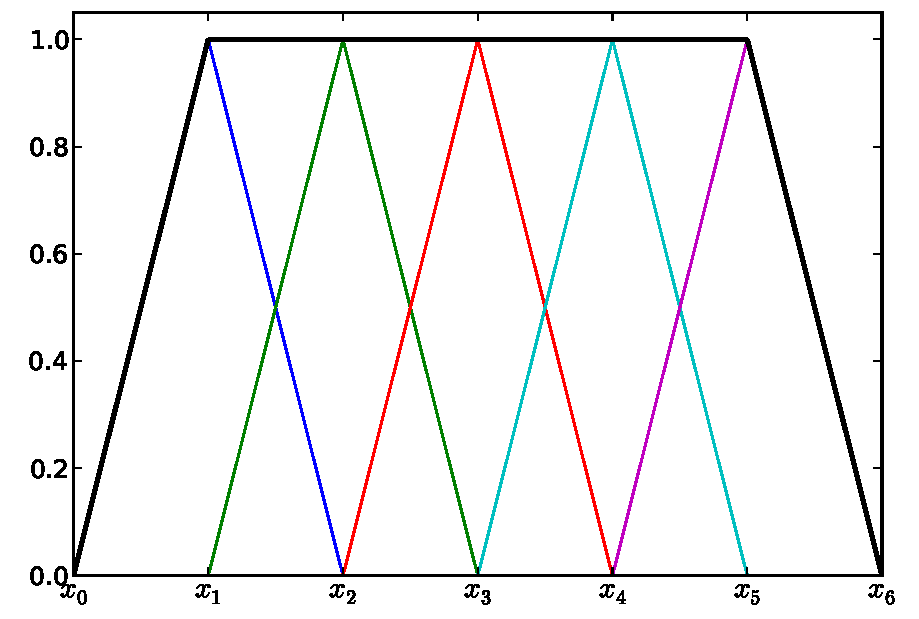
\includegraphics[scale=0.4]{Fig00_BSplines_Int_D1.pdf}
  \end{center}
  \vspace{-20pt}
  \caption{\footnotesize ToFu-created $d=1$ bsplines}
  \vspace{-10pt}
\end{wrapfigure}

$$
\begin{array}{lll}
& \int_{x_k}^{x_{k+1}} g^2(x)dx\\
= & \frac{x_{k+1}-x_k}{2}\sum_{i=1}^n w_i \left(c_{k-1}b_{1,k-1}\left(X_{i,k}\right) + c_{k}b_{1,k}\left(X_{i,k}\right)\right)^2\\
= & \frac{x_{k+1}-x_k}{2}\sum_{i=1}^n w_i \left(c_{k-1}^2b_{1,k-1}^2\left(X_{i,k}\right) + 2c_{k-1}c_{k}b_{1,k-1}\left(X_{i,k}\right)b_{1,k}\left(X_{i,k}\right) + c_{k}^2b_{1,k}^2\left(X_{i,k}\right) + \right)\\
= & c_{k-1}^2\frac{x_{k+1}-x_k}{2}\sum_{i=1}^n w_ib_{1,k-1}^2\left(X_{i,k}\right) + 2c_{k-1}c_{k}\frac{x_{k+1}-x_k}{2}\sum_{i=1}^n w_ib_{1,k-1}\left(X_{i,k}\right)b_{1,k}\left(X_{i,k}\right) + c_{k}^2\frac{x_{k+1}-x_k}{2}\sum_{i=1}^n w_ib_{1,k}^2\left(X_{i,k}\right)\\
= & c_{k-1}^2A_{k-1,k-1,k} + 2c_{k-1}c_{k}A_{k-1,k,k} + c_{k}^2A_{k,k,k}
\end{array}
$$

Hence, by summing over all intervals:
$$
\begin{array}{llll}
\int_{a}^{b} g^2(x)dx & = & c_{0}^2\int_{x_0}^{x_{1}}b_{2,0}^2 & (k=0)\\
&& + c_{0}^2\int_{x_1}^{x_{2}}b_{2,0}^2 + c_{1}^2\int_{x_1}^{x_{2}}b_{2,1}^2 + 2c_{0}c_{1}\int_{x_1}^{x_{2}}b_{2,0}b_{2,1} & (k=1)\\
&& + c_{1}^2\int_{x_2}^{x_{3}}b_{2,1}^2 + c_{2}^2\int_{x_2}^{x_{3}}b_{2,2}^2 + 2c_{1}c_{2}\int_{x_2}^{x_{3}}b_{2,1}b_{2,2} & (k=2)\\
&& + c_{2}^2\int_{x_3}^{x_{4}}b_{2,2}^2 + c_{3}^2\int_{x_3}^{x_{4}}b_{2,3}^2 + 2c_{2}c_{3}\int_{x_3}^{x_{4}}b_{2,2}b_{2,3} & (k=3)\\
&& + \hdots &\\
& = & c_{0}^2\int_{I_0}b_{2,0}^2 + 2c_{0}c_{1}\int_{I_0\bigcap I_1}b_{2,0}b_{2,1} + c_{1}^2\int_{I_1}b_{2,1}^2 + 2c_{1}c_{2}\int_{I_1\bigcap I_2}b_{2,1}b_{2,2} + \hdots&
\end{array}
$$

Where we have introduce $I_j$ the interval on which $b_{1,j}$ lives. Thus noting $A_{i,j} = \int_{I_i\bigcap I_j}b_{2,i}b_{2,j} = A_{j,i}$.

$$
\int_{a}^{b} g^2(x)dx = ^t\underline{C}\underline{\underline{A}}\underline{C} = ^t\underline{C} \left(\begin{array}{ccccccc} \int_{I_0}b_{1,0}^2&A_{0,1}&&&&&\\ A_{0,1}&\ddots&\ddots&&&&\\ &\ddots&\ddots&A_{j,j-1}&&&\\ &&A_{j,j-1}&\int_{I_j}b_{1,j}^2&A_{j,j+1}&&\\ &&&A_{j,j+1}&\ddots&\ddots&\\ &&&&\ddots&\ddots&A_{N-2,N-1}\\ &&&&&A_{N-2,N-1}&\int_{I_{N-1}}b_{1,N-1}^2 \end{array}\right) \underline{C}\\
$$


\newpage
\paragraph{\textbf{$d=2$ $\Rightarrow$ 3 b-splines on each interval $n=3$ ($2\times2=4$)}}

Following the same logic, we have here for each interval:

\begin{wrapfigure}{r}{0.5\textwidth}
  \vspace{-20pt}
  \begin{center}
    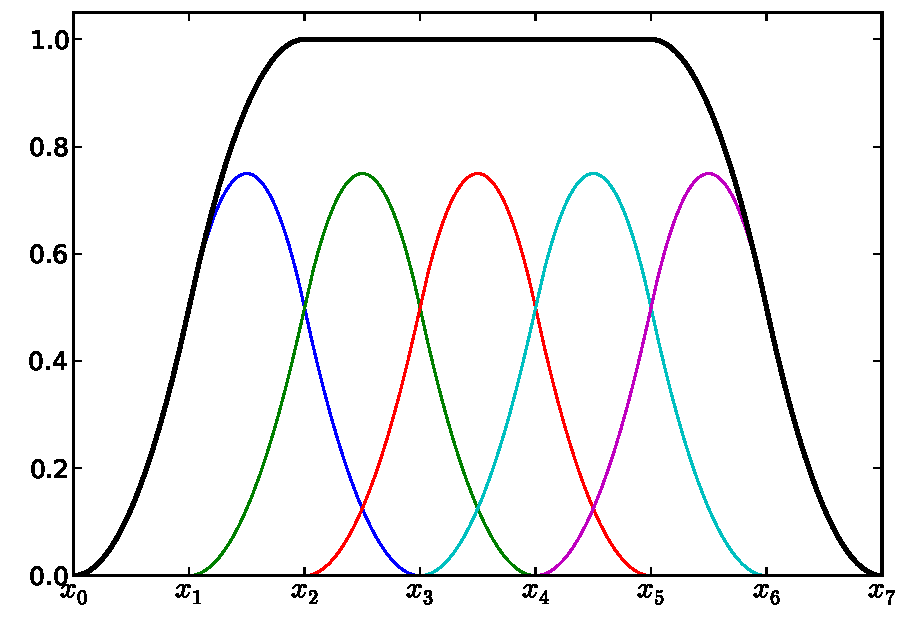
\includegraphics[scale=0.4]{Fig01_BSplines_Int_D2.pdf}
  \end{center}
  \vspace{-20pt}
  \caption{\footnotesize ToFu-created $d=2$ bsplines}
  \vspace{-10pt}
\end{wrapfigure}

$$
\begin{array}{lll}
& \int_{x_k}^{x_{k+1}} g^2(x)dx\\
= & \int_{x_k}^{x_{k+1}} \left( c_{k-2}b_{2,k-2} + c_{k-1}b_{2,k-1} + c_{k}b_{2,k} \right)^2(x)dx \\
= & \int_{x_k}^{x_{k+1}} c_{k-2}^2b_{2,k-2}^2 + c_{k-1}^2b_{2,k-1}^2 + 2c_{k-2}b_{2,k-2}c_{k-1}b_{2,k-1} + c_{k}^2b_{2,k}^2 + 2c_{k}b_{2,k}c_{k-2}b_{2,k-2} + 2c_{k}b_{2,k}c_{k-1}b_{2,k-1} \\
= & c_{k-2}^2\int_{x_k}^{x_{k+1}}b_{2,k-2}^2 + c_{k-1}^2\int_{x_k}^{x_{k+1}}b_{2,k-1}^2 + c_{k}^2\int_{x_k}^{x_{k+1}}b_{2,k}^2 ...\\
  &  + 2c_{k-2}c_{k-1}\int_{x_k}^{x_{k+1}}b_{2,k-2}b_{2,k-1} + 2c_{k}c_{k-2}\int_{x_k}^{x_{k+1}}b_{2,k}b_{2,k-2} + 2c_{k}c_{k-1}\int_{x_k}^{x_{k+1}}b_{2,k}b_{2,k-1}
\end{array}
$$

Hence, by summing over all intervals:
$$
\begin{array}{llll}
\int_{a}^{b} g^2(x)dx & = & c_{0}^2\int_{x_0}^{x_{1}}b_{2,0}^2 & (k=0)\\
&& + c_{0}^2\int_{x_1}^{x_{2}}b_{2,0}^2 + c_{1}^2\int_{x_1}^{x_{2}}b_{2,1}^2 + 2c_{0}c_{1}\int_{x_1}^{x_{2}}b_{2,0}b_{2,1} & (k=1)\\
&& + c_{0}^2\int_{x_2}^{x_{3}}b_{2,0}^2 + c_{1}^2\int_{x_2}^{x_{3}}b_{2,1}^2 + c_{2}^2\int_{x_2}^{x_{3}}b_{2,2}^2 + 2c_{0}c_{1}\int_{x_2}^{x_{3}}b_{2,0}b_{2,1} + 2c_{0}c_{2}\int_{x_2}^{x_{3}}b_{2,0}b_{2,2} + 2c_{1}c_{2}\int_{x_2}^{x_{3}}b_{2,1}b_{2,2} & (k=2)\\
&& + c_{1}^2\int_{x_3}^{x_{4}}b_{2,1}^2 + c_{2}^2\int_{x_3}^{x_{4}}b_{2,2}^2 + c_{3}^2\int_{x_3}^{x_{4}}b_{2,3}^2 + 2c_{1}c_{2}\int_{x_3}^{x_{4}}b_{2,1}b_{2,2} + 2c_{1}c_{3}\int_{x_3}^{x_{4}}b_{2,1}b_{2,3} + 2c_{2}c_{3}\int_{x_3}^{x_{4}}b_{2,2}b_{2,3} & (k=3)\\
&& + \hdots &\\
& = & c_{0}^2\int_{I_0}b_{2,0}^2 + 2c_{0}c_{1}\int_{I_0\bigcap I_1}b_{2,0}b_{2,1} + 2c_{0}c_{2}\int_{I_0\bigcap I_2}b_{2,0}b_{2,2} + c_{1}^2\int_{I_1}b_{2,1}^2 + 2c_{1}c_{2}\int_{I_1\bigcap I_2}b_{2,1}b_{2,2} + \hdots&
\end{array}
$$


So in matrix form, still noting $A_{i,j} = \int_{I_i\bigcap I_j}b_{2,i}b_{2,j} = A_{j,i}$:
$$
\int_{a}^{b} g^2(x)dx = ^t\underline{C}\underline{\underline{A}}\underline{C} = ^t\underline{C} \left(\begin{array}{ccccccccccc}
\int_{I_0}b_{2,0}^2&A_{0,1}&A_{0,2}&&&&&&&&\\ A_{0,1}&\ddots&\ddots&\ddots&&&&&&&\\ A_{0,2}&\ddots&\ddots&\ddots&\ddots&&&&&&\\
&\ddots&\ddots&\ddots&\ddots&A_{j,j-2}&&&&&\\ &&\ddots&\ddots&\ddots&A_{j,j-1}&\ddots&&&&\\
&&&A_{j,j-2}&A_{j,j-1}&\int_{I_j}b_{2,j}^2&A_{j,j+1}&A_{j,j+2}&&&\\
&&&&\ddots&A_{j,j+1}&\ddots&\ddots&\ddots&&\\ &&&&&A_{j,j+2}&\ddots&\ddots&\ddots&\ddots&\\
&&&&&&\ddots&\ddots&\ddots&\ddots&A_{N-1,N-3}\\ &&&&&&&\ddots&\ddots&\ddots&A_{N-1,N-2}\\ &&&&&&&&A_{N-1,N-3}&A_{N-1,N-2}&\int_{I_{N-1}}b_{2,N-1}^2
\end{array}\right) \underline{C}\\
$$

\newpage
\paragraph{\textbf{$d=3$ $\Rightarrow$ 4 b-splines on each interval $n=4$ ($2\times3=6$)}}

The degree determines the amount of overlapping (i.e.: the number of non-zero diagonals in the matrix).
Apart from that, the rest remains similar since we are still deriving the squared total function.

\begin{wrapfigure}{r}{0.4\textwidth}
  \vspace{-20pt}
  \begin{center}
    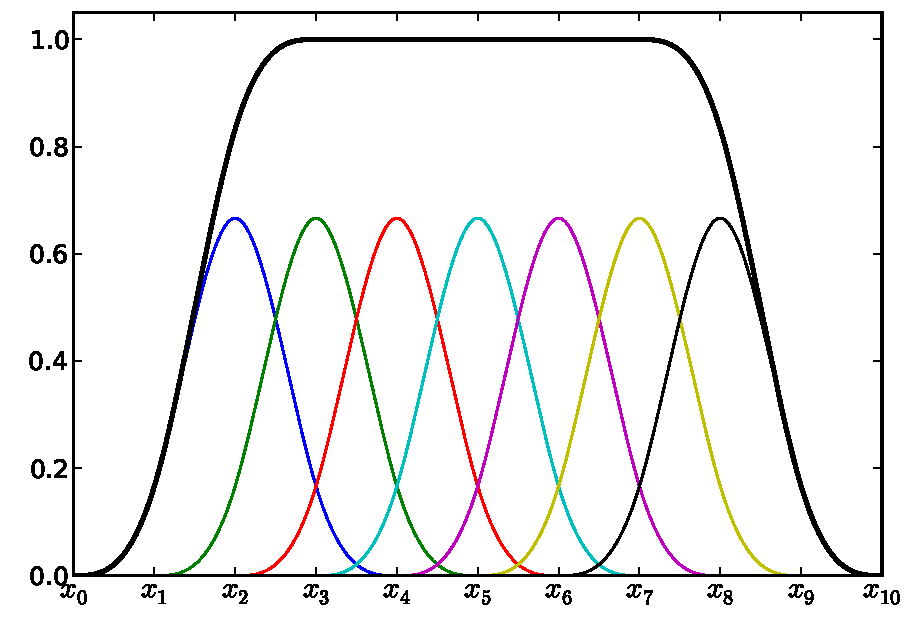
\includegraphics[scale=0.4]{Fig02_BSplines_Int_D3.pdf}
  \end{center}
  \vspace{-20pt}
  \caption{\footnotesize ToFu-created $d=3$ bsplines}
  \vspace{-10pt}
\end{wrapfigure}

$$
\begin{array}{lll}
& \int_{x_k}^{x_{k+1}} g^2(x)dx\\
= & \int_{x_k}^{x_{k+1}} \left( c_{k-3}b_{3,k-3} + c_{k-2}b_{3,k-2} + c_{k-1}b_{3,k-1} + c_{k}b_{3,k} \right)^2(x)dx\\
= & c_{k-3}^2\int_{x_k}^{x_{k+1}}b_{3,k-3}^2 + c_{k-2}^2\int_{x_k}^{x_{k+1}}b_{3,k-2}^2 + c_{k-1}^2\int_{x_k}^{x_{k+1}}b_{3,k-1}^2 + c_{k}^2\int_{x_k}^{x_{k+1}}b_{3,k}^2 ...\\
  & + 2c_{k-3}c_{k-2}\int_{x_k}^{x_{k+1}}b_{3,k-3}b_{3,k-2} + 2c_{k-3}c_{k-1}\int_{x_k}^{x_{k+1}}b_{3,k-3}b_{3,k-1} + 2c_{k-3}c_{k}\int_{x_k}^{x_{k+1}}b_{3,k-3}b_{3,k} ...\\
  & + 2c_{k-2}c_{k-1}\int_{x_k}^{x_{k+1}}b_{3,k-2}b_{3,k-1} + 2c_{k}c_{k-2}\int_{x_k}^{x_{k+1}}b_{3,k}b_{3,k-2} + 2c_{k}c_{k-1}\int_{x_k}^{x_{k+1}}b_{3,k}b_{3,k-1}
\end{array}
$$

hence, following the same logic:

$$
\int_{a}^{b} g^2(x)dx = ^t\underline{C}\underline{\underline{A}}\underline{C} = ^t\underline{C} \left(\begin{array}{ccccccccccccccc}
\int_{I_0}b_{3,0}^2&A_{0,1}&A_{0,2}&A_{0,3}&&&&&&&&&&&\\ A_{0,1}&\ddots&\ddots&\ddots&\ddots&&&&&&&&&&\\ A_{0,2}&\ddots&\ddots&\ddots&\ddots&\ddots&&&&&&&&&\\ A_{0,3}&\ddots&\ddots&\ddots&\ddots&\ddots&\ddots&&&&&&&&\\
&\ddots&\ddots&\ddots&\ddots&\ddots&\ddots&A_{j,j-3}&&&&&&&\\ &&\ddots&\ddots&\ddots&\ddots&\ddots&A_{j,j-2}&\ddots&&&&&&\\ &&&\ddots&\ddots&\ddots&\ddots&A_{j,j-1}&\ddots&\ddots&&&&&\\
&&&&A_{j,j-3}&A_{j,j-2}&A_{j,j-1}&\int_{I_j}b_{3,j}^2&A_{j,j+1}&A_{j,j+2}&A_{j,j+3}&&&&\\
&&&&&\ddots&\ddots&A_{j,j+1}&\ddots&\ddots&\ddots&&&&\\ &&&&&&\ddots&A_{j,j+2}&\ddots&\ddots&\ddots&\ddots&&&\\ &&&&&&&A_{j,j+3}&\ddots&\ddots&\ddots&\ddots&\ddots&&\\
&&&&&&&&&\ddots&\ddots&\ddots&\ddots&\ddots&A_{N-1,N-4}\\ &&&&&&&&&&\ddots&\ddots&\ddots&\ddots&A_{N-1,N-3}\\
&&&&&&&&&&&\ddots&\ddots&\ddots&A_{N-1,N-2}\\ &&&&&&&&&&&A_{N-1,N-4}&A_{N-1,N-3}&A_{N-1,N-2}&\int_{I_{N-1}}b_{3,N-1}^2
\end{array}\right) \underline{C}\\
$$

\newpage
\subsubsection{D1N2}

With squared derivatives of any order, the structure of A, determined by the number of overlaps, is identical to $D0N2$.
However, the integrands are the chosen derivatives, and computing each integral requires less quadrature points per mesh element (smaller degree).\\
Here $A_{i,j} = \int_{I_i\bigcap I_j}\partial_xb_{d,i}\partial_xb_{d,j} = A_{j,i}$

\paragraph{\textbf{$d=1$ $\Rightarrow$ 2 b-splines on each interval $n=1$ ($2\times0=0$)}}
$$
\int_{a}^{b} \left(\partial_x g\right)^2 = ^t\underline{C} \left(\begin{array}{ccccccc}
\int_{I_0}\left(\partial_xb_{1,0}\right)^2&A_{0,1}&&&&&\\ A_{0,1}&\ddots&\ddots&&&&\\
&\ddots&\ddots&A_{j,j-1}&&&\\ &&A_{j,j-1}&\int_{I_j}\left(\partial_xb_{1,j}\right)^2&A_{j,j+1}&&\\ &&&A_{j,j+1}&\ddots&\ddots&\\
&&&&\ddots&\ddots&A_{N-2,N-1}\\ &&&&&A_{N-2,N-1}&\int_{I_{N-1}}\left(\partial_xb_{1,N-1}\right)^2
\end{array}\right) \underline{C}\\
$$

\paragraph{\textbf{$d=2$ $\Rightarrow$ 3 b-splines on each interval $n=2$ ($2\times1=2$)}}
$$
\int_{a}^{b} \left(\partial_xg\right)^2 = ^t\underline{C} \left(\begin{array}{ccccccccccc}
\int_{I_0}\left(\partial_xb_{2,0}\right)^2&A_{0,1}&A_{0,2}&&&&&&&&\\ A_{0,1}&\ddots&\ddots&\ddots&&&&&&&\\ A_{0,2}&\ddots&\ddots&\ddots&\ddots&&&&&&\\
&\ddots&\ddots&\ddots&\ddots&A_{j,j-2}&&&&&\\ &&\ddots&\ddots&\ddots&A_{j,j-1}&\ddots&&&&\\
&&&A_{j,j-2}&A_{j,j-1}&\int_{I_j}\left(\partial_xb_{2,j}\right)^2&A_{j,j+1}&A_{j,j+2}&&&\\
&&&&\ddots&A_{j,j+1}&\ddots&\ddots&\ddots&&\\ &&&&&A_{j,j+2}&\ddots&\ddots&\ddots&\ddots&\\
&&&&&&\ddots&\ddots&\ddots&\ddots&A_{N-1,N-3}\\ &&&&&&&\ddots&\ddots&\ddots&A_{N-1,N-2}\\ &&&&&&&&A_{N-1,N-3}&A_{N-1,N-2}&\int_{I_{N-1}}\left(\partial_xb_{2,N-1}\right)^2
\end{array}\right) \underline{C}\\
$$

\paragraph{\textbf{$d=3$ $\Rightarrow$ 4 b-splines on each interval $n=3$ ($2\times2=4$)}}
$$
\int_{a}^{b} \left(\partial_xg\right)^2 = ^t\underline{C} \left(\begin{array}{ccccccccccccccc}
\int_{I_0}\left(\partial_xb_{3,0}\right)^2&A_{0,1}&A_{0,2}&A_{0,3}&&&&&&&&&&&\\ A_{0,1}&\ddots&\ddots&\ddots&\ddots&&&&&&&&&&\\ A_{0,2}&\ddots&\ddots&\ddots&\ddots&\ddots&&&&&&&&&\\ A_{0,3}&\ddots&\ddots&\ddots&\ddots&\ddots&\ddots&&&&&&&&\\
&\ddots&\ddots&\ddots&\ddots&\ddots&\ddots&A_{j,j-3}&&&&&&&\\ &&\ddots&\ddots&\ddots&\ddots&\ddots&A_{j,j-2}&\ddots&&&&&&\\ &&&\ddots&\ddots&\ddots&\ddots&A_{j,j-1}&\ddots&\ddots&&&&&\\
&&&&A_{j,j-3}&A_{j,j-2}&A_{j,j-1}&\int_{I_j}\left(\partial_xb_{3,j}\right)^2&A_{j,j+1}&A_{j,j+2}&A_{j,j+3}&&&&\\
&&&&&\ddots&\ddots&A_{j,j+1}&\ddots&\ddots&\ddots&&&&\\ &&&&&&\ddots&A_{j,j+2}&\ddots&\ddots&\ddots&\ddots&&&\\ &&&&&&&A_{j,j+3}&\ddots&\ddots&\ddots&\ddots&\ddots&&\\
&&&&&&&&&\ddots&\ddots&\ddots&\ddots&\ddots&A_{N-1,N-4}\\ &&&&&&&&&&\ddots&\ddots&\ddots&\ddots&A_{N-1,N-3}\\
&&&&&&&&&&&\ddots&\ddots&\ddots&A_{N-1,N-2}\\ &&&&&&&&&&&A_{N-1,N-4}&A_{N-1,N-3}&A_{N-1,N-2}&\int_{I_{N-1}}\left(\partial_xb_{3,N-1}\right)^2
\end{array}\right) \underline{C}\\
$$

\subsubsection{D2N2}
Here again, A has the same structure, but the integrals can be evaluated with fewer points and $A_{i,j} = \int_{I_i\bigcap I_j}\partial^2_xb_{d,i}\partial^2_xb_{d,j} = A_{j,i}$
\paragraph{\textbf{$d=2$ $\Rightarrow$ 3 b-splines on each interval $n=1$ ($2\times0=0$)}}
\paragraph{\textbf{$d=3$ $\Rightarrow$ 4 b-splines on each interval $n=2$ ($2\times1=2$)}}

\subsubsection{D3N2}
Here again, A has the same structure, but the integrals can be evaluated with fewer points and $A_{i,j} = \int_{I_i\bigcap I_j}\partial^3_xb_{3,i}\partial^3_xb_{3,j} = A_{j,i}$
\paragraph{\textbf{$d=3$ $\Rightarrow$ 4 b-splines on each interval $n=1$ ($2\times0=0$)}}

\end{landscape}
\newpage
\subsection{Non-linear functionals}

In this section, we consider two non-linear functionals: the entropy (D0ME) and the Fisher information (D1FI).\\
Obviously, the non-linearity prevents from building a matrix operator. Instead, we simply want to assess the value of the integral as fast as possible for one set of coefficients.\\
Since there is no quadrature rule dedicated to these expressions (here $g$ is a sum of b-splines of degree 0,1,2 or 3), we resort to the Gauss-Legendre quadrature, with possibly more points that would be required based on the degree of $g$.


\subsubsection{D0ME}

Applicable to all degrees, $D0ME\left(g\right) = -\int g\ln(g)$.\\
However, the entropy is in principle computed with a distribution, so alternatively: $D0ME\left(g\right) = -\int \frac{g}{\int g}\ln\left(\frac{g}{\int g}\right)$.\\

Since in most cases the considered function $g$ will decrease to 0 at the edge of the domain, it may be necessary to introduce a threshold value $\epsilon$ below which the term in the natural logarithm is replaced by $\epsilon$:

$$
D0ME\left(g\right) = - \left[\int_{g\geq \epsilon} \frac{g}{\int g}\ln\left(\frac{g}{\int g}\right) + \int_{g<\epsilon} \frac{g}{\int g}\ln\left(\frac{\epsilon}{\int g}\right) \right]
$$

The value of $\epsilon$ is an input, provided as an absolute value, as a fraction of $\max(g)$ or of $\int g$.
Finally, we also use teh absolute value of $g$ to be able to apply the same method to negative profiles, with $\epsilon$ defined from $\max(\|g\|)$ or of $\int \|g\|$:

$$
D0ME\left(g\right) = - \left[\int_{\|g\|\geq \epsilon} \frac{\|g\|}{\int \|g\|}\ln\left(\frac{\|g\|}{\int \|g\|}\right) + \int_{\|g\|<\epsilon} \frac{\|g\|}{\int \|g\|}\ln\left(\frac{\epsilon}{\int \|g\|}\right) \right]
$$


\subsubsection{D1FI}

Applicable to degrees $d \geq 1$, $D1FI\left(g\right) = \int \frac{\left(\partial_x g\right)^2}{g}$ or optionally (experimental): $\int \frac{\left(\partial_x g\right)^2}{\|g\|}$\\
However, the same numerical problem arises: if $g$ goes to $0$ the integral diverges or is dominated by its weakest values, hence we also introduce a threshold $\epsilon$ from $\max(\|g\|)$ or of $\int \|g\|$:
$$
D1FI\left(g\right) = \int_{\|g\|\geq \epsilon} \frac{\|\partial_x g\|^2}{\|g\|} + \int_{\|g\|<\epsilon} \frac{\|\partial_x g\|^2}{\epsilon}
$$




\newpage
\section{2D b-splines}



\newpage
\appendix
\begin{landscape}
\section{D0,D1,D2,D3 - Surf - Exact formulations}


\subsection{Deriv = 0 - Deg = 0}
$$
\int_{x_0}^{x_1} b_{0,0}(x) dx = \int_{x_0}^{x_1} dx = x_1-x_0
$$


\subsection{Deriv = 0 - Deg = 1}
$$
\begin{array}{lll}
\int_{x_0}^{x_2} b_{1,0}(x) dx & = \int_{x_0}^{x_1} \frac{x-x_0}{x_1-x_0}dx + \int_{x_1}^{x_2} \frac{x_2-x}{x_2-x_1}dx\\
& = \frac{\left[(x-x_0)^2\right]_{x_0}^{x_1}}{2(x_1-x_0)} + \frac{\left[-(x_2-x)^2\right]_{x_1}^{x_2}}{2(x_2-x_1)}\\
& = \frac{(x_1-x_0)^2}{2(x_1-x_0)} + \frac{(x_2-x_1)^2}{2(x_2-x_1)}
& = \frac{x_2-x_0}{2}
\end{array}
$$

\subsection{Deriv = 0 - Deg = 2}

$$
\begin{array}{lll}
\int_{x_0}^{x_3} b_{2,0}(x) dx & = \int_{x_0}^{x_1} \frac{(x-x_0)^2}{(x_2-x_0)(x_1-x0)} dx
+ \int_{x_1}^{x_2} \frac{(x-x_0)(x_2-x)}{(x_2-x_0)(x_2-x_1)} + \frac{(x-x_1)(x_3-x)}{(x_2-x_1)(x_3-x_1)}dx
+ \int_{x_2}^{x_3} \frac{(x_3-x)^2}{(x_3-x_2)(x_3-x_1)}dx\\

& = \frac{\left[\frac{(x-x_0)^3}{3}\right]_{x_0}^{x_1}}{(x_2-x_0)(x_1-x0)}
+ \frac{\left[-\frac{x^3}{3} + (x_0+x_2)\frac{x^2}{2} - xx_0x_2\right]_{x_1}^{x_2}}{(x_2-x_0)(x_2-x_1)}  +  \frac{ \left[-\frac{x^3}{3} + (x_1+x_3)\frac{x^2}{2} -xx_1x_3\right]_{x_1}^{x_2} }{(x_2-x_1)(x_3-x_1)}
+ \frac{-\left[\frac{(x_3-x)^3}{3}\right]_{x_2}^{x_3}}{(x_3-x_2)(x_3-x_1)}\\

& = \frac{(x_1-x_0)^2}{3(x_2-x_0)}
+ \frac{-\frac{x_2^2+x_2x_1+x_1^2}{3} + (x_0+x_2)\frac{x_2+x_1}{2} - x_0x_2}{(x_2-x_0)}
+ \frac{ -\frac{x_2^2+x_2x_1+x_1^2}{3} + (x_1+x_3)\frac{x_2+x_1}{2} -x_1x_3 }{(x_3-x_1)}
+ \frac{(x_3-x_2)^2}{3(x_3-x_1)}\\

& = \frac{(x_1-x_0)^2}{3(x_2-x_0)}
+ \frac{ -2(x_2^2+x_2x_1+x_1^2) + 3(x_0+x_2)(x_2+x_1) - 6x_0x_2}{6(x_2-x_0)}
+ \frac{ -2(x_2^2+x_2x_1+x_1^2) + 3(x_1+x_3)(x_2+x_1) - 6x_1x_3}{6(x_3-x_1)}
+ \frac{(x_3-x_2)^2}{3(x_3-x_1)}\\

& = \frac{(x_1-x_0)^2}{3(x_2-x_0)}
+ \frac{ x_2^2 + x_2x_1 - 2x_1^2 + 3x_0(x_1-x_2)}{6(x_2-x_0)}
+ \frac{ -2x_2^2 + x_2x_1 + x_1^2 + 3x_3(x_2-x_1)}{6(x_3-x_1)}
+ \frac{(x_3-x_2)^2}{3(x_3-x_1)}

\end{array}
$$


\subsection{Deriv = 0 - Deg = 3}

$$
b_{3,0} =
\left\{
\begin{array}{lll}
\frac{x^3 - 3x^2x_0 + 3xx_0^2 - x_0^3}{(x_3-x_0)(x_2-x_0)(x_1-x_0)} & \text{ ,  if  } & x \in [x_0,x_1[\\
\frac{x^3A + x^2B + xC + D}{(x_4-x_1)(x_3-x_1)(x_3-x_0)(x_2-x_1)(x_2-x_0)} & \text{ ,  if  } & x \in [x_1,x_2[\\
\frac{x^3A^/ + x^2B^/ + xC^/ + D^/}{(x_4-x_2)(x_4-x_1)(x_3-x_2)(x_3-x_1)(x_3-x_0)} & \text{ ,  if  } & x \in [x_2,x_3[\\
\frac{-x^3 + 3x^2x_4 - 3xx_4^2 + x_4^3}{(x_4-x_3)(x_4-x_2)(x_4-x_1)} & \text{ ,  if  } & x \in [x_3,x_4[
\end{array}
\right.
$$


Hence

$$
\begin{array}{lll}
\int_{x_0}^{x_4} b & = & \int_{x_0}^{x_1} b + \int_{x_1}^{x_2} b + \int_{x_2}^{x_3} b + \int_{x_3}^{x_4} b\\
& = & \int_{x_0}^{x_1} \frac{x^3 - 3x^2x_0 + 3xx_0^2 - x_0^3}{(x_3-x_0)(x_2-x_0)(x_1-x_0)}
+ \int_{x_1}^{x_2} \frac{x^3A + x^2B + xC + D}{(x_4-x_1)(x_3-x_1)(x_3-x_0)(x_2-x_1)(x_2-x_0)}
+ \int_{x_2}^{x_3} \frac{x^3A^/ + x^2B^/ + xC^/ + D^/}{(x_4-x_2)(x_4-x_1)(x_3-x_2)(x_3-x_1)(x_3-x_0)}
+ \int_{x_3}^{x_4} \frac{-x^3 + 3x^2x_4 - 3xx_4^2 + x_4^3}{(x_4-x_3)(x_4-x_2)(x_4-x_1)} \\
& = &  \frac{\frac{x_1^4-x_0^4}{4} - 3x_0\frac{x_1^3-x_0^3}{3} + 3x_0^2\frac{x_1^2-x_0^2}{2} - x_0^3(x_1-x_0)}{(x_3-x_0)(x_2-x_0)(x_1-x_0)}
+ \frac{A\frac{x_2^4-x_1^4}{4} + B\frac{x_2^3-x_1^3}{3} + C\frac{x_2^2-x_1^2}{2} + D(x_2-x_1)}{(x_4-x_1)(x_3-x_1)(x_3-x_0)(x_2-x_1)(x_2-x_0)}
+ \frac{A^/\frac{x_3^4-x_2^4}{4} + x^2B^/\frac{x_3^3-x_2^3}{3} + C^/\frac{x_3^2-x_2^2}{2} + D^/(x_3-x_2)}{(x_4-x_2)(x_4-x_1)(x_3-x_2)(x_3-x_1)(x_3-x_0)}
+ \frac{-\frac{x_4^4-x_3^4}{4} + 3x_4\frac{x_4^3-x_3^3}{3} - 3x_4^2\frac{x_4^2-x_3^2}{2} + x_4^3(x_4-x_3)}{(x_4-x_3)(x_4-x_2)(x_4-x_1)}
\end{array}
$$

\subsection{Deriv = 1 - Deg = 2}

$$
\begin{array}{lll}

\int_{x_0}^{x_3} \partial_x b_{2,0} & =
\left\{
\begin{array}{llll}
\frac{2}{2(x_2-x_0)(x_1-x_0)}\int_{x_0}^{x_1} (x-x_0)^2 dx && \text{ ,  on } & [x_0,x_1[\\
\frac{\int_{x_1}^{x_2} -2x(x_3+x_2-x_1-x_0) + 2(x_3x_2-x_1x_0) dx}{(x_2-x_1)(x_2-x_0)(x_3-x_1)} & = \frac{\left[-x^2(x_3+x_2-x_1-x_0) + 2x(x_3x_2-x_1x_0)\right]_{x_1}^{x_2}}{(x_2-x_1)(x_2-x_0)(x_3-x_1)} & \text{ ,  on } & [x_1,x_2[\\
\frac{-2}{-2(x_3-x_2)(x_3-x_1)}\int_{x_2}^{x_3} (x_3-x)^2 dx && \text{ ,  on } & [x_2,x_3[
\end{array}
\right.\\

& = \left\{
\begin{array}{lll}
\frac{x_1-x_0}{x_2-x_0} & \text{ ,  on } & [x_0,x_1[\\
\frac{-x_3x_2^2-x_2^3+x_2^2x_1+x_2^2x_0 + 2x_3x_2^2-2x_2x_1x_0 + x_3x_1^2+x_2x_1^2-x_1^3-x_1^2x_0 - 2x_3x_2x_1-2x_1^2x_0}{(x_2-x_1)(x_2-x_0)(x_3-x_1)} & \text{ ,  on } & [x_1,x_2[\\
-\frac{x_3-x_2}{x_3-x_1} & \text{ ,  on } & [x_2,x_3[
\end{array}
\right.\\

& = \left\{
\begin{array}{lll}
\frac{x_1-x_0}{x_2-x_0} & \text{ ,  on } & [x_0,x_1[\\
\frac{ x_3x_2^2 - x_2^3 + x_2^2x_1 + x_2^2x_0 - 2x_2x_1x_0 + x_3x_1^2 + x_2x_1^2 - x_1^3 - 2x_3x_2x_1 + x_1^2x_0 }{(x_2-x_1)(x_2-x_0)(x_3-x_1)} & \text{ ,  on } & [x_1,x_2[\\
-\frac{x_3-x_2}{x_3-x_1} & \text{ ,  on } & [x_2,x_3[
\end{array}
\right.

\end{array}
$$

\subsection{Deriv = 1 - Deg = 3}

$$
\begin{array}{lll}

\int_{x_0}^{x_4} \partial_x b_{3,0}

& = \left\{
\begin{array}{llll}
 & \int_{x_0}^{x_1} \frac{3x^2 - 6xx_0 + 3x_0^2}{(x_3-x_0)(x_2-x_0)(x_1-x_0)} & \text{ ,  on } & [x_0,x_1[\\
 & \int_{x_1}^{x_2} \frac{3x^2A + 2xB + C}{(x_4-x_1)(x_3-x_1)(x_3-x_0)(x_2-x_1)(x_2-x_0)} & \text{ ,  on } & [x_1,x_2[\\
 & \int_{x_2}^{x_3} \frac{3x^2A^/ + 2xB^/ + C^/}{(x_4-x_2)(x_4-x_1)(x_3-x_2)(x_3-x_1)(x_3-x_0)} & \text{ ,  on } & [x_2,x_3[\\
 & \int_{x_3}^{x_4} \frac{-3x^2 + 6xx_4 - 3x_4^2}{(x_4-x_3)(x_4-x_2)(x_4-x_1)} & \text{ ,  on } & [x_3,x_4[\\
\end{array}
\right.\\

& = \frac{\left[ x^3 - 3x^2x_0 + 3x_0^2x \right]_{x_0}^{x_1}}{(x_3-x_0)(x_2-x_0)(x_1-x_0)}
+ \frac{\left[ x^3A + x^2B + Cx \right]_{x_1}^{x_2}}{(x_4-x_1)(x_3-x_1)(x_3-x_0)(x_2-x_1)(x_2-x_0)}
+ \frac{\left[ x^3A^/ + x^2B^/ + C^/x \right]_{x_2}^{x_3}}{(x_4-x_2)(x_4-x_1)(x_3-x_2)(x_3-x_1)(x_3-x_0)}
+ \frac{\left[ -x^3 + 3x^2x_4 - 3x_4^2x \right]_{x_3}^{x_4}}{(x_4-x_3)(x_4-x_2)(x_4-x_1)}\\

& = \frac{ (x_1^3-x_0^3) - 3x_0(x_1^2-x_0^2) + 3x_0^2(x_1-x_0) }{(x_3-x_0)(x_2-x_0)(x_1-x_0)}
+ \frac{ A(x_2^3-x_1^3) + B(x_2^2-x_1^2) + C(x_2-x_1)}{(x_4-x_1)(x_3-x_1)(x_3-x_0)(x_2-x_1)(x_2-x_0)}
+ \frac{ A^/(x_3^3-x_1^3) + B^/(x_3^2-x_2^2) + C^/(x_3-x_2) }{(x_4-x_2)(x_4-x_1)(x_3-x_2)(x_3-x_1)(x_3-x_0)}
+ \frac{-(x_4^3-x_3^3) + 3x_4(x_4^2-x_3^2) - 3x_4^2(x_4-x_3)}{(x_4-x_3)(x_4-x_2)(x_4-x_1)}

\end{array}
$$


\subsection{Deriv = 2 - Deg = 3}

$$
\begin{array}{lll}

\int_{x_0}^{x_4} \partial_x^2 b_{3,0}

& = \left\{
\begin{array}{llll}
 & \int_{x_0}^{x_1} \frac{6x - 6x_0}{(x_3-x_0)(x_2-x_0)(x_1-x_0)} & \text{ ,  on } & [x_0,x_1[\\
 & \int_{x_1}^{x_2} \frac{6xA + 2B}{(x_4-x_1)(x_3-x_1)(x_3-x_0)(x_2-x_1)(x_2-x_0)} & \text{ ,  on } & [x_1,x_2[\\
 & \int_{x_2}^{x_3} \frac{6xA^/ + 2B^/}{(x_4-x_2)(x_4-x_1)(x_3-x_2)(x_3-x_1)(x_3-x_0)} & \text{ ,  on } & [x_2,x_3[\\
 & \int_{x_3}^{x_4} \frac{-6x + 6x_4}{(x_4-x_3)(x_4-x_2)(x_4-x_1)} & \text{ ,  on } & [x_3,x_4[\\
\end{array}
\right.\\

& = \frac{ 3(x_1^2-x_0^2) - 6x_0(x_1-x_0) }{(x_3-x_0)(x_2-x_0)(x_1-x_0)}
+ \frac{ 3A(x_2^2-x_1^2) + 2B(x_2-x_1) }{(x_4-x_1)(x_3-x_1)(x_3-x_0)(x_2-x_1)(x_2-x_0)}
+ \frac{ 3A^/(x_3^2-x_1^2) + 2B^/(x_3-x_2) }{(x_4-x_2)(x_4-x_1)(x_3-x_2)(x_3-x_1)(x_3-x_0)}
+ \frac{ -3(x_4^2-x_3^2) + 6x_4(x_4-x_3)}{(x_4-x_3)(x_4-x_2)(x_4-x_1)}\\

& = \frac{ 3(x_1-x_0) }{(x_3-x_0)(x_2-x_0)}
+ \frac{ 3A(x_2^2-x_1^2) + 2B(x_2-x_1) }{(x_4-x_1)(x_3-x_1)(x_3-x_0)(x_2-x_1)(x_2-x_0)}
+ \frac{ 3A^/(x_3^2-x_1^2) + 2B^/(x_3-x_2) }{(x_4-x_2)(x_4-x_1)(x_3-x_2)(x_3-x_1)(x_3-x_0)}
+ \frac{ 3(x_4-x_3)}{(x_4-x_2)(x_4-x_1)}

\end{array}
$$

\subsection{Deriv = 3 - Deg = 3}

$$
\begin{array}{lll}

\int_{x_0}^{x_4} \partial_x^3 b_{3,0}

& = \left\{
\begin{array}{llll}
 & \int_{x_0}^{x_1} \frac{6}{(x_3-x_0)(x_2-x_0)(x_1-x_0)} & \text{ ,  on } & [x_0,x_1[\\
 & \int_{x_1}^{x_2} \frac{6A}{(x_4-x_1)(x_3-x_1)(x_3-x_0)(x_2-x_1)(x_2-x_0)} & \text{ ,  on } & [x_1,x_2[\\
 & \int_{x_2}^{x_3} \frac{6A^/}{(x_4-x_2)(x_4-x_1)(x_3-x_2)(x_3-x_1)(x_3-x_0)} & \text{ ,  on } & [x_2,x_3[\\
 & \int_{x_3}^{x_4} \frac{-6}{(x_4-x_3)(x_4-x_2)(x_4-x_1)} & \text{ ,  on } & [x_3,x_4[\\
\end{array}
\right.\\

& = \frac{ 6 }{(x_3-x_0)(x_2-x_0)}
+ \frac{ 6A(x_2-x_1) }{(x_4-x_1)(x_3-x_1)(x_3-x_0)(x_2-x_1)(x_2-x_0)}
+ \frac{ 6A^/(x_3-x_2) }{(x_4-x_2)(x_4-x_1)(x_3-x_2)(x_3-x_1)(x_3-x_0)}
+ \frac{ -6}{(x_4-x_2)(x_4-x_1)}\\

\end{array}
$$


\newpage
\section{D0,D1,D2,D3 - Vol - Exact formulations}

\subsection{Deriv = 0 - Deg = 0}
$$
\int_{x_0}^{x_1} xb_{0,0}(x) dx = \int_{x_0}^{x_1} xdx = \frac{x_1^2-x_0^2}{2}
$$


\subsection{Deriv = 0 - Deg = 1}
$$
\begin{array}{lll}
\int_{x_0}^{x_2} xb_{1,0}(x) dx & = \int_{x_0}^{x_1} x\frac{x-x_0}{x_1-x_0}dx + \int_{x_1}^{x_2} x\frac{x_2-x}{x_2-x_1}dx\\
& = \frac{1}{x_1-x_0}\left[ \frac{x^3}{3} - x_0\frac{x^2}{2} \right]_{x_0}^{x_1} + \frac{1}{x_2-x_1}\left[ x_2\frac{x^2}{2} - \frac{x^3}{3} \right]_{x_1}^{x_2}\\
& = \frac{1}{x_1-x_0}\left( \frac{x_1^3-x_0^3}{3} - x_0\frac{x_1^2-x_0^2}{2} \right) + \frac{1}{x_2-x_1}\left( x_2\frac{x_2^2-x_1^2}{2} - \frac{x_2^3-x_1^3}{3} \right)\\
& = \left( \frac{x_1^2+x_1x_0+x_0^2}{3} - x_0\frac{x_1+x_0}{2} \right) + \left( x_2\frac{x_2+x_1}{2} - \frac{x_2^2+x_2x_1+x_1^2}{3} \right)\\
& = \frac{2x_1^2 - x_1x_0 - x_0^2}{6} + \frac{x_2^2 + x_2x_1 - 2x_1^2}{6}
& = \frac{x_2^2 + x_1(x_2-x_0) - x_0^2}{6}
\end{array}
$$


\subsection{Deriv = 0 - Deg = 2}


$$
\begin{array}{lll}
\int_{x_0}^{x_3} xb_{2,0}(x) dx & = & \int_{x_0}^{x_1} x\frac{(x-x_0)^2}{(x_2-x_0)(x_1-x0)} dx
+ \int_{x_1}^{x_2} x\frac{(x-x_0)(x_2-x)}{(x_2-x_0)(x_2-x_1)} + x\frac{(x-x_1)(x_3-x)}{(x_2-x_1)(x_3-x_1)}dx
+ \int_{x_2}^{x_3} x\frac{(x_3-x)^2}{(x_3-x_2)(x_3-x_1)}dx\\

& = & \frac{\left[ \frac{x^4}{4}-2x_0\frac{x^3}{3}+x_0^2\frac{x^2}{2} \right]_{x_0}^{x_1}}{(x_2-x_0)(x_1-x0)}
+ \frac{\left[-\frac{x^4}{4} + (x_0+x_2)\frac{x^3}{3} - x_0x_2\frac{x^2}{2}\right]_{x_1}^{x_2}}{(x_2-x_0)(x_2-x_1)} + \frac{ \left[-\frac{x^4}{4} + (x_1+x_3)\frac{x^3}{3} -x_1x_3\frac{x^2}{2}\right]_{x_1}^{x_2} }{(x_2-x_1)(x_3-x_1)}
+ \frac{\left[ \frac{x^4}{4}-2x_3\frac{x^3}{3}+x_3^2\frac{x^2}{2} \right]_{x_2}^{x_3}}{(x_3-x_2)(x_3-x_1)}\\

& = & \frac{ 3(x_1^4-x_0^4) - 8x_0(x_1^3-x_0^3) + 6x_0^2(x_1^2-x_0^2) }{12(x_2-x_0)(x_1-x0)}
+ \frac{ -3(x_2^4-x_1^4) + 4(x_0+x_2)(x_2^3-x_1^3) - 6x_0x_2(x_2^2-x_1^2) }{12(x_2-x_0)(x_2-x_1)}
+ \frac{ -3(x_2^4-x_1^4) + 4(x_1+x_3)(x_2^3-x_1^3) -6x_1x_3(x_2^2-x_1^2) }{12(x_2-x_1)(x_3-x_1)}
+ \frac{  3(x_3^4-x_2^2) - 8x_3(x_3^3-x_2^3) + 6x_3^2(x_3^2-x_2^2) }{12(x_3-x_2)(x_3-x_1)}\\

& = & \frac{ 3(x_1^2+x_0^2)(x_1+x_0) - 8x_0(x_1^2+x_1x_0+x_0^2) + 6x_0^2(x_1+x_0) }{ 12(x_2-x_0) }\\
&& + \frac{ -3(x_2^2+x_1^2)(x_2+x_1) + 4(x_0+x_2)(x_2^2+x_2x_1+x_1^2) - 6x_0x_2(x_2+x_1) }{ 12(x_2-x_0) }
   + \frac{ -3(x_2^2+x_1^2)(x_2+x_1) + 4(x_1+x_3)(x_2^2+x_2x_1+x_1^2) - 6x_1x_3(x_2+x_1) }{ 12(x_3-x_1) }\\
&& + \frac{  3(x_3^2+x_2^2)(x_3+x_2) - 8x_3(x_3^2+x_3x_2+x_2^2) + 6x_3^2(x_3+x_2) }{ 12(x_3-x_1) }\\

& = & \frac{ 3x_1^3 + 3x_0^2x_1 + 3x_0x_1^2 + 3x_0^3 - 8x_0x_1^2 - 8x_0^2x_1 - 8x_0^3 + 6x_0^2x_1 + 6x_0^3 }{ 12(x_2-x_0) }\\
&& + \frac{ -3x_2^3 - 3x_1x_2^2 - 3x_1^2x_2 - 3x_1^3 + 4x_0x_2^2 + 4x_0x_1x_2 + 4x_0x_1^2 + 4x_2^3 + 4x_2^2x_1 + 4x_1^2x_2 - 6x_0x_2^2 - 6x_0x_1x_2 }{ 12(x_2-x_0) }
   + \frac{ -3x_2^3 - 3x_1x_2^2 - 3x_1^2x_2 - 3x_1^3 + 4x_1x_2^2 + 4x_1^2x_2 + 4x_1^3 + 4x_2^2x_3 + 4x_1x_2x_3 + 4x_1^2x_3 - 6x_1x_2x_3 - 6x_1^2x_3 }{ 12(x_3-x_1) }\\
&& + \frac{  3x_3^3 + 3x_2x_3^2 + 3x_2^2x_3 + 3x_2^3 - 8x_3^3 - 8x_2x_3^2 - 8x_2^2x_3 + 6x_3^3 + 6x_2x_3^2 }{ 12(x_3-x_1) }\\

& = & \frac{ 3x_1^3 + x_0^2x_1 - 5x_0x_1^2 + x_0^3 }{ 12(x_2-x_0) }\\
&& + \frac{  x_2^3 + x_1x_2^2 + x_1^2x_2 - 3x_1^3 - 2x_0x_2^2 - 2x_0x_1x_2 + 4x_0x_1^2 }{ 12(x_2-x_0) }
   + \frac{ -3x_2^3 + x_1x_2^2 + x_1^2x_2 + x_1^3 + 4x_2^2x_3 - 2x_1x_2x_3 - 2x_1^2x_3 }{ 12(x_3-x_1) }\\
&& + \frac{  x_3^3 + x_2x_3^2 - 5x_2^2x_3 + 3x_2^3 }{ 12(x_3-x_1) }\\

& = & \frac{ (3x_1+x_0)(x_1-x_0)^2 }{ 12(x_2-x_0) }
+ \frac{ (x_2-x_1)\left( x_2^2+2x_1x_2+3x_1^2 - 2x_0(x_2+2x_1) \right) }{ 12(x_2-x_0) }
- \frac{ (x_2-x_1)\left( x_1^2+2x_1x_2+3x_2^2 - 2x_3(2x_2+x_1) \right) }{ 12(x_3-x_1) }
+ \frac{ (3x_2+x_3)(x_3-x_2)^2 }{ 12(x_3-x_1) }


\end{array}
$$



\subsection{Deriv = 0 - Deg = 3}


$$
\begin{array}{lll}

\int_{x_0}^{x_4} xb_{3,0}(x) dx & = & \int_{x_0}^{x_1} x\frac{x^3-3x_0x^2+3x_0^2x-x_0^3}{(x_3-x_0)(x_2-x_0)(x_1-x_0)} dx
+ \int_{x_1}^{x_2} x\frac{Ax^3+Bx^2+Cx+D}{(x_4-x_1)(x_3-x_1)(x_3-x_0)(x_2-x_1)(x_2-x_0)} dx
+ \int_{x_2}^{x_3} x\frac{A^/x^3+B^/x^2+C^/x+D^/}{(x_4-x_2)(x_4-x_1)(x_3-x_2)(x_3-x_1)(x_3-x_0)} dx
+ \int_{x_3}^{x_4} x\frac{-x^3+3x_4x^2-3x_4^2x+x_4^3}{(x_4-x_3)(x_4-x_2)(x_4-x_1)} dx\\

& = & \frac{\left[ \frac{x^5}{5} - 3x_0\frac{x^4}{4} + 3x_0^2\frac{x^3}{3} - x_0^3\frac{x^2}{2} \right]_{x_0}^{x_1}}{(x_3-x_0)(x_2-x_0)(x_1-x_0)}
+ \frac{\left[ A\frac{x^5}{5} + B\frac{x^4}{4} + C\frac{x^3}{3} + D\frac{x^2}{2} \right]_{x_1}^{x_2}}{(x_4-x_1)(x_3-x_1)(x_3-x_0)(x_2-x_1)(x_2-x_0)}
+ \frac{\left[ A^/\frac{x^5}{5} + B^/\frac{x^4}{4} + C^/\frac{x^3}{3} + D^/\frac{x^2}{2} \right]_{x_2}^{x_3}}{(x_4-x_2)(x_4-x_1)(x_3-x_2)(x_3-x_1)(x_3-x_0)}
+ \frac{\left[ -\frac{x^5}{5} + 3x_4\frac{x^4}{4} - 3x_4^2\frac{x^3}{3} + x_4^3\frac{x^2}{2} \right]_{x_3}^{x_4}}{(x_4-x_3)(x_4-x_2)(x_4-x_1)}\\

& = & \frac{ 12(x_1^5-x_0^5) - 45x_0(x_1^4-x_0^4) + 60x_0^2(x_1^3-x_0^3) - 30x_0^3(x_1^2-x_0^2) }{60(x_3-x_0)(x_2-x_0)(x_1-x_0)}\\
&& + \frac{ 12A(x_2^5-x_1^5) + 15B(x_2^4-x_1^4) + 20C(x_2^3-x_1^3) + 30D(x_2^2-x_1^2) }{60(x_4-x_1)(x_3-x_1)(x_3-x_0)(x_2-x_1)(x_2-x_0)}\\
&& + \frac{ 12A^/(x_3^5-x_2^5) + 15B^/(x_3^4-x_2^4) + 20C^/(x_3^3-x_2^3) + 30D^/(x_3^2-x_2^2) }{60(x_4-x_2)(x_4-x_1)(x_3-x_2)(x_3-x_1)(x_3-x_0)}\\
&& + \frac{ -12(x_4^5-x_3^5) + 45x_4(x_4^4-x_3^4) - 60x_4^2(x_4^3-x_3^3) + 30x_4^3(x_4^2-x_3^2) }{60(x_4-x_3)(x_4-x_2)(x_4-x_1)}\\

\end{array}
$$


\subsection{Deriv = 1 - Deg = 1}

$$
\begin{array}{lll}
\int_{x_0}^{x_2} x \partial_x b_{1,0}(x) dx & = \int_{x_0}^{x_1} x\frac{1}{x_1-x_0}dx - \int_{x_1}^{x_2} x\frac{1}{x_2-x_1}dx\\
& = \frac{x_1^2-x_0^2}{2(x_1-x_0)} - \frac{x_2^2-x_1^2}{2(x_2-x_1)}\\
& = \frac{x_1+x_0}{2} - \frac{x_2+x_1}{2}
& = -\frac{x_2-x_0}{2}
\end{array}
$$


\subsection{Deriv = 1 - Deg = 2}

$$
\begin{array}{lll}
\int_{x_0}^{x_3} xb_{2,0}(x) dx & = & \int_{x_0}^{x_1} x\frac{2(x-x_0)}{(x_2-x_0)(x_1-x0)} dx
+ \int_{x_1}^{x_2} x\frac{-2x + (x_2+x_0)}{(x_2-x_0)(x_2-x_1)} + x\frac{-2x + (x_3+x_1)}{(x_2-x_1)(x_3-x_1)}dx
+ \int_{x_2}^{x_3} x\frac{-2(x_3-x)}{(x_3-x_2)(x_3-x_1)}dx\\

& = & 2\frac{ \left[ \frac{x^3}{3}-x_0\frac{x^2}{2} \right]_{x_0}^{x_1} }{(x_2-x_0)(x_1-x0)}
+ \frac{\left[ -2\frac{x^3}{3} + (x_2+x_0)\frac{x^2}{2} \right]_{x_1}^{x_2} }{(x_2-x_0)(x_2-x_1)}
+ \frac{\left[ -2\frac{x^3}{3} + (x_3+x_1)\frac{x^2}{2} \right]_{x_1}^{x_2} }{(x_2-x_1)(x_3-x_1)}
+ 2\frac{\left[ \frac{x^3}{3} - x_3\frac{x^2}{2} \right]_{x_2}^{x_3}}{(x_3-x_2)(x_3-x_1)}\\

& = & 2\frac{ 2(x_1^3-x_0^3) - 3x_0(x_1^2-x_0^2) }{6(x_2-x_0)(x_1-x0)}
+ \frac{ -4(x_2^3-x_1^3) + 3(x_2+x_0)(x_2^2-x_1^2) }{6(x_2-x_0)(x_2-x_1)}
+ \frac{ -4(x_2^3-x_1^3) + 3(x_3+x_1)(x_2^2-x_1^2) }{6(x_2-x_1)(x_3-x_1)}
+ 2\frac{ 2(x_3^3-x_2^3) - 3x_3(x_3^2-x_2^2) }{6(x_3-x_2)(x_3-x_1)}\\

& = & 2\frac{ 2(x_1^2+x_1x_0+x_0^2) - 3x_0(x_1+x_0) }{6(x_2-x_0)}
+ \frac{ -4(x_2^2+x_2x_1+x_1^2) + 3(x_2+x_0)(x_2+x_1) }{6(x_2-x_0)}
+ \frac{ -4(x_2^2+x_2x_1+x_1^2) + 3(x_3+x_1)(x_2+x_1) }{6(x_3-x_1)}
+ 2\frac{ 2(x_3^2+x_3x_2+x_2^2) - 3x_3(x_3+x_2) }{6(x_3-x_1)}\\

& = & \frac{ 2x_1^2 - x_1x_0 - x_0^2 }{3(x_2-x_0)}
+ \frac{ -x_2^2 - x_2x_1 - 4x_1^2 + 3x_0x_2 + 3x_0x_1 }{6(x_2-x_0)}
+ \frac{ -4x_2^2 - x_2x_1 - x_1^2 + 3x_3x_2 + 3x_3x_1 }{6(x_3-x_1)}
+ \frac{ -x_3^2 - x_3x_2 + 2x_2^2 }{3(x_3-x_1)}
\end{array}
$$


\subsection{Deriv = 1 - Deg = 3}

$$
\begin{array}{lll}

\int_{x_0}^{x_4} xb_{3,0}(x) dx & = & \int_{x_0}^{x_1} x\frac{3x^2-6x_0x+3x_0^2}{(x_3-x_0)(x_2-x_0)(x_1-x_0)} dx
+ \int_{x_1}^{x_2} x\frac{3Ax^2+2Bx+C}{(x_4-x_1)(x_3-x_1)(x_3-x_0)(x_2-x_1)(x_2-x_0)} dx
+ \int_{x_2}^{x_3} x\frac{3A^/x^2+2B^/x+C^/}{(x_4-x_2)(x_4-x_1)(x_3-x_2)(x_3-x_1)(x_3-x_0)} dx
+ \int_{x_3}^{x_4} x\frac{-3x^2+6x_4x-3x_4^2}{(x_4-x_3)(x_4-x_2)(x_4-x_1)} dx\\

& = & \frac{\left[ 3\frac{x^4}{4} - 6x_0\frac{x^3}{3} + 3x_0^2\frac{x^2}{2} \right]_{x_0}^{x_1}}{(x_3-x_0)(x_2-x_0)(x_1-x_0)}
+ \frac{\left[ 3A\frac{x^4}{4} + 2B\frac{x^3}{3} + C\frac{x^2}{2} \right]_{x_1}^{x_2}}{(x_4-x_1)(x_3-x_1)(x_3-x_0)(x_2-x_1)(x_2-x_0)}
+ \frac{\left[ 3A^/\frac{x^4}{4} + 2B^/\frac{x^3}{3} + C^/\frac{x^2}{2} \right]_{x_2}^{x_3}}{(x_4-x_2)(x_4-x_1)(x_3-x_2)(x_3-x_1)(x_3-x_0)}
+ \frac{\left[ -3\frac{x^4}{4} + 6x_4\frac{x^3}{3} - 3x_4^2\frac{x^2}{2}  \right]_{x_3}^{x_4}}{(x_4-x_3)(x_4-x_2)(x_4-x_1)}\\

& = & \frac{ 9(x_1^4-x_0^4) - 24x_0(x_1^3-x_0^3) + 18x_0^2(x_1^2-x_0^2) }{12(x_3-x_0)(x_2-x_0)(x_1-x_0)}
+ \frac{ 9A(x_2^4-x_1^4) + 8B(x_2^3-x_1^3) + 6C(x_2^2-x_1^2) }{12(x_4-x_1)(x_3-x_1)(x_3-x_0)(x_2-x_1)(x_2-x_0)}
+ \frac{ 9A^/(x_3^4-x_2^4) + 8B^/(x_3^3-x_2^3) + 6C^/(x_3^2-x_2^3) }{12(x_4-x_2)(x_4-x_1)(x_3-x_2)(x_3-x_1)(x_3-x_0)}
+ \frac{ -9(x_4^4-x_3^4) + 24x_4(x_4^3-x_3^3) - 18x_4^2(x_4^2-x_3^2) }{12(x_4-x_3)(x_4-x_2)(x_4-x_1)}\\

& = & \frac{ 9(x_1^2+x_0^2)(x_1+x_0) - 24x_0(x_1^2+x_1x_0+x_0^2) + 18x_0^2(x_1+x_0) }{12(x_3-x_0)(x_2-x_0)}
+ \frac{ 9A(x_2^4-x_1^4) + 8B(x_2^3-x_1^3) + 6C(x_2^2-x_1^2) }{12(x_4-x_1)(x_3-x_1)(x_3-x_0)(x_2-x_1)(x_2-x_0)}
+ \frac{ 9A^/(x_3^4-x_2^4) + 8B^/(x_3^3-x_2^3) + 6C^/(x_3^2-x_2^3) }{12(x_4-x_2)(x_4-x_1)(x_3-x_2)(x_3-x_1)(x_3-x_0)}
+ \frac{ -9(x_4^2+x_3^2)(x_4+x_3) + 24x_4(x_4^2+x_4x_3+x_3^2) - 18x_4^2(x_4+x_3) }{12(x_4-x_2)(x_4-x_1)}\\

& = & \frac{ 3x_1^3 - 5x_1^2x_0 + x_1x_0^2 + x_0^3 }{4(x_3-x_0)(x_2-x_0)}
+ \frac{ 9A(x_2^4-x_1^4) + 8B(x_2^3-x_1^3) + 6C(x_2^2-x_1^2) }{12(x_4-x_1)(x_3-x_1)(x_3-x_0)(x_2-x_1)(x_2-x_0)}
+ \frac{ 9A^/(x_3^4-x_2^4) + 8B^/(x_3^3-x_2^3) + 6C^/(x_3^2-x_2^3) }{12(x_4-x_2)(x_4-x_1)(x_3-x_2)(x_3-x_1)(x_3-x_0)}
+ \frac{ -x_4^3 + 5x_4x_3^2 - x_4^2x_3 - 3x_3^3 }{4(x_4-x_2)(x_4-x_1)}\\

\end{array}
$$




\subsection{Deriv = 2 - Deg = 2}

$$
\begin{array}{lll}
\int_{x_0}^{x_3} xb_{2,0}(x) dx & = & \int_{x_0}^{x_1} x\frac{2}{(x_2-x_0)(x_1-x0)} dx
+ \int_{x_1}^{x_2} x\frac{-2}{(x_2-x_0)(x_2-x_1)} + x\frac{-2}{(x_2-x_1)(x_3-x_1)}dx
+ \int_{x_2}^{x_3} x\frac{2}{(x_3-x_2)(x_3-x_1)}dx\\

& = & \frac{(x_1^2-x_0^2)}{(x_2-x_0)(x_1-x0)}
- \frac{x_2^2-x_1^2}{(x_2-x_0)(x_2-x_1)} - \frac{x_2^2-x_1^2}{(x_2-x_1)(x_3-x_1)}
+ \frac{x_3^2-x_2^2}{(x_3-x_2)(x_3-x_1)}\\

& = & \frac{x_1+x_0}{x_2-x_0} - \frac{x_2+x_1}{x_2-x_0} - \frac{x_2+x_1}{x_3-x_1} + \frac{x_3+x_2}{x_3-x_1}
\end{array}
$$


\subsection{Deriv = 2 - Deg = 3}

$$
\begin{array}{lll}

\int_{x_0}^{x_4} xb_{3,0}(x) dx & = & \int_{x_0}^{x_1} x\frac{ 6x - 6x_0 }{(x_3-x_0)(x_2-x_0)(x_1-x_0)} dx
+ \int_{x_1}^{x_2} x\frac{6Ax + 2B}{(x_4-x_1)(x_3-x_1)(x_3-x_0)(x_2-x_1)(x_2-x_0)} dx
+ \int_{x_2}^{x_3} x\frac{6A^/x + 2B^/}{(x_4-x_2)(x_4-x_1)(x_3-x_2)(x_3-x_1)(x_3-x_0)} dx
+ \int_{x_3}^{x_4} x\frac{-6x + 6x_4}{(x_4-x_3)(x_4-x_2)(x_4-x_1)} dx\\

& = & \frac{\left[ 6\frac{x^3}{3} - 6x_0\frac{x^2}{2} \right]_{x_0}^{x_1}}{(x_3-x_0)(x_2-x_0)(x_1-x_0)}
+ \frac{\left[ 6A\frac{x^3}{3} + 2B\frac{x^2}{2} \right]_{x_1}^{x_2}}{(x_4-x_1)(x_3-x_1)(x_3-x_0)(x_2-x_1)(x_2-x_0)}
+ \frac{\left[ 6A^/\frac{x^3}{3} + 2B^/\frac{x^2}{2} \right]_{x_2}^{x_3}}{(x_4-x_2)(x_4-x_1)(x_3-x_2)(x_3-x_1)(x_3-x_0)}
+ \frac{\left[ -6\frac{x^3}{3} + 6x_4\frac{x^2}{2} \right]_{x_3}^{x_4}}{(x_4-x_3)(x_4-x_2)(x_4-x_1)}\\

& = & \frac{ 12(x_1^3-x_0^3) - 18x_0(x_1^2-x_0^2) }{6(x_3-x_0)(x_2-x_0)(x_1-x_0)}
+ \frac{12A(x_2^3-x_1^3) + 6B(x_2^2-x_1^2)}{6(x_4-x_1)(x_3-x_1)(x_3-x_0)(x_2-x_1)(x_2-x_0)}
+ \frac{12A^/(x_3^3-x_2^3) + 6B^/(x_3^2-x_2^2)}{6(x_4-x_2)(x_4-x_1)(x_3-x_2)(x_3-x_1)(x_3-x_0)}
+ \frac{-12(x_4^3-x_3^3) + 18x_4(x_4^2-x_3^2)}{6(x_4-x_3)(x_4-x_2)(x_4-x_1)}\\

& = & \frac{ 2x_1^2 - x_1x_0 - x_0^2 }{(x_3-x_0)(x_2-x_0)}
+ \frac{2A(x_2^3-x_1^3) + B(x_2^2-x_1^2)}{(x_4-x_1)(x_3-x_1)(x_3-x_0)(x_2-x_1)(x_2-x_0)}
+ \frac{2A^/(x_3^3-x_2^3) + B^/(x_3^2-x_2^2)}{(x_4-x_2)(x_4-x_1)(x_3-x_2)(x_3-x_1)(x_3-x_0)}
+ \frac{x_4^2 + x_4x_3 - 2x_3^2}{(x_4-x_2)(x_4-x_1)}

\end{array}
$$


\subsection{Deriv = 3 - Deg = 3}

$$
\begin{array}{lll}

\int_{x_0}^{x_4} xb_{3,0}(x) dx & = & \int_{x_0}^{x_1} x\frac{ 6 }{(x_3-x_0)(x_2-x_0)(x_1-x_0)} dx
+ \int_{x_1}^{x_2} x\frac{6A}{(x_4-x_1)(x_3-x_1)(x_3-x_0)(x_2-x_1)(x_2-x_0)} dx
+ \int_{x_2}^{x_3} x\frac{6A^/}{(x_4-x_2)(x_4-x_1)(x_3-x_2)(x_3-x_1)(x_3-x_0)} dx
+ \int_{x_3}^{x_4} x\frac{-6}{(x_4-x_3)(x_4-x_2)(x_4-x_1)} dx\\

& = & \frac{ 3(x_1^2-x_0^2) }{(x_3-x_0)(x_2-x_0)(x_1-x_0)}
+ \frac{3A(x_2^2-x_1^2)}{(x_4-x_1)(x_3-x_1)(x_3-x_0)(x_2-x_1)(x_2-x_0)}
+ \frac{3A^/(x_3^2-x_2^2)}{(x_4-x_2)(x_4-x_1)(x_3-x_2)(x_3-x_1)(x_3-x_0)}
+ \frac{-3(x_4^2-x_3^2)}{(x_4-x_3)(x_4-x_2)(x_4-x_1)}\\

& = & \frac{ 3(x_1+x_0) }{(x_3-x_0)(x_2-x_0)}
+ \frac{3A(x_2^2-x_1^2)}{(x_4-x_1)(x_3-x_1)(x_3-x_0)(x_2-x_1)(x_2-x_0)}
+ \frac{3A^/(x_3^2-x_2^2)}{(x_4-x_2)(x_4-x_1)(x_3-x_2)(x_3-x_1)(x_3-x_0)}
- \frac{3(x_4+x_3)}{(x_4-x_2)(x_4-x_1)}

\end{array}
$$


\newpage
\section{D0N2 - Exact formulations}

\subsection{Deg = 0, Surf}
$$
\int_{x_0}^{x_1} \|b_{0,0}(x)\|^2 dx = \int_{x_0}^{x_1} dx = x_1-x_0
$$

\subsection{Deg = 0, Vol}
$$
\int_{x_0}^{x_1} x\|b_{0,0}(x)\|^2 dx = \int_{x_0}^{x_1} x dx = \frac{x_1^2-x_0^2}{2}
$$

\subsection{Deg = 1, Surf}
$$
\begin{array}{llll}
\int_{x_0}^{x_2} \|b_{1,0}(x)\|^2 dx & = & \int_{x_0}^{x_1} \left(\frac{x-x_0}{x_1-x_0}\right)^2  dx + \int_{x_1}^{x_2} \left(\frac{x_2-x}{x_2-x_1}\right)^2  dx\\
& = & \frac{\left[ \frac{(x-x_0)^3}{3} \right]_{x_0}^{x_1} }{(x_1-x_0)^2} + \frac{\left[ -\frac{(x_2-x)^3}{3} \right]_{x_1}^{x_2} }{(x_2-x_1)^2}\\
& = & \frac{x_1-x_0}{3} + \frac{x_2-x_1}{3}
& = \frac{x_2-x_0}{3}
\end{array}
$$

and

$$
\begin{array}{llll}
\int_{x_1}^{x_2} b_{1,0}(x)\times b_{1,1}(x) dx & = & \int_{x_1}^{x_2} \frac{x_2-x}{x_2-x_1}\frac{x-x_1}{x_2-x_1}  dx\\
& = & \frac{\left[ -\frac{x^3}{3} + (x_2+x_1)\frac{x^2}{2} - x_2x_1x \right]_{x_1}^{x_2}}{(x_2-x_1)^2}\\
& = & \frac{ -2(x_2^3-x_1^3) + 3(x_2+x_1)(x_2^2-x_1^2) - 6x_2x_1(x_2-x_1) }{6(x_2-x_1)^2}\\
& = & \frac{ -2(x_2^2+x_2x_1+x_1^2) + 3(x_2+x_1)(x_2+x_1) - 6x_2x_1 }{6(x_2-x_1)}\\
& = & \frac{ -2x_2^2 - 2x_2x_1 - 2x_1^2 + 3x_2^2 + 6x_2x_1 + 3x_1^2 - 6x_2x_1 }{6(x_2-x_1)}\\
& = & \frac{ x_2^2 - 2x_2x_1 + x_1^2 }{6(x_2-x_1)}
& = \frac{x_2 - x_1}{6}
\end{array}
$$

\subsection{Deg = 1, Vol}
$$
\begin{array}{lll}
\int_{x_0}^{x_2} x\|b_{1,0}(x)\|^2 dx & = & \int_{x_0}^{x_1} x\left(\frac{x-x_0}{x_1-x_0}\right)^2  dx + \int_{x_1}^{x_2} x\left(\frac{x_2-x}{x_2-x_1}\right)^2  dx\\
& = & \frac{\left[ \frac{x^4}{4} - 2x_0\frac{x^3}{3} + x_0^2\frac{x^2}{2} \right]_{x_0}^{x_1} }{(x_1-x_0)^2} + \frac{\left[ \frac{x^4}{4} - 2x_2\frac{x^3}{3} + x_2^2\frac{x^2}{2} \right]_{x_1}^{x_2} }{(x_2-x_1)^2}\\
& = & \frac{ 3(x_1^4-x_0^4) - 8x_0(x_1^3-x_0^3) + 6x_0^2(x_1^2-x_0^2) }{12(x_1-x_0)^2} + \frac{ 3(x_2^4-x_1^4) - 8x_2(x_2^3-x_1^3) + 6x_2^2(x_2^2-x_1^2) }{12(x_2-x_1)^2}\\
& = & \frac{ 3(x_1^2+x_0^2)(x_1+x_0) - 8x_0(x_1^2+x_1x_0+x_0^2) + 6x_0^2(x_1+x_0) }{12(x_1-x_0)} + \frac{ 3(x_2^2+x_1^2)(x_2+x_1) - 8x_2(x_2^2+x_2x_1+x_1^2) + 6x_2^2(x_2+x_1) }{12(x_2-x_1)}\\
& = & \frac{ 3x_1^3 + 3x_1^2x_0 + 3x_0^2x_1 + 3x_0^3 - 8x_0x_1^2 - 8x_1x_0^2 - 8x_0^3 + 6x_0^2x_1+6x_0^3 }{12(x_1-x_0)}
+ \frac{ 3x_2^3 + 3x_2^2x_1 + 3x_2x_1^2 + 3x_1^3 - 8x_2^3 - 8x_2^2x_1 - 8x_2x_1^2 + 6x_2^3 + 6x_2^2x_1 }{12(x_2-x_1)}\\
& = & \frac{ 3x_1^3 - 5x_1^2x_0 + x_0^2x_1 + x_0^3 }{12(x_1-x_0)} + \frac{x_2^3 + x_2^2x_1 - 5x_2x_1^2 + 3x_1^3 }{12(x_2-x_1)}\\
& = & \frac{ 
    (3x_1^3 - 5x_1^2x_0 + x_0^2x_1 + x_0^3)(x_2-x_1)
    + (x_2^3 + x_2^2x_1 - 5x_2x_1^2 + 3x_1^3)(x_1-x_0)
    }{12(x_1-x_0)(x_2-x_1)}\\
& = & \frac{ 
    x_2(3x_1^3 - 5x_1^2x_0 + x_0^2x_1 + x_0^3)
    + x_1(x_2^3 + x_2^2x_1 - 5x_2x_1^2 + 5x_1^2x_0 - x_0^2x_1 - x_0^3)
    - x_0(x_2^3 + x_2^2x_1 - 5x_2x_1^2 + 3x_1^3)
    }{12(x_1-x_0)(x_2-x_1)}\\
\end{array}
$$

and

$$
\begin{array}{llll}
\int_{x_1}^{x_2} xb_{1,0}(x)\times b_{1,1}(x) dx & = & \int_{x_1}^{x_2} x\frac{x_2-x}{x_2-x_1}\frac{x-x_1}{x_2-x_1}  dx\\
& = & \frac{\left[ -\frac{x^4}{4} + (x_2+x_1)\frac{x^3}{3} - x_2x_1\frac{x^2}{2} \right]_{x_1}^{x_2}}{(x_2-x_1)^2}\\
& = & \frac{ -3(x_2^4-x_1^4) + 4(x_2+x_1)(x_2^3-x_1^3) - 6x_2x_1(x_2^2-x_1^2) }{12(x_2-x_1)^2}\\
& = & \frac{ -3(x_2^2+x_1^2)(x_2+x_1) + 4(x_2+x_1)(x_2^2+x_2x_1+x_1^2) - 6x_2x_1(x_2+x_1) }{12(x_2-x_1)}\\
& = & \frac{ -3x_2^3 - 3x_2x_1^2 - 3x_2^2x_1 - 3x_1^3 + 4x_2^3 + 4x_2^2x_1 + 4x_2x_1^2 + 4x_2^2x_1 + 4x_2x_1^2 + 4x_1^3 - 6x_2^2x_1 - 6x_2x_1^2 }{12(x_2-x_1)}\\
& = & \frac{ x_2^2-x_1^2 }{12}\\
\end{array}
$$

\subsection{Deg = 2, Surf}

$$
\begin{array}{lll}
\int_{x_0}^{x_3} \|b_{2,0}(x)\|^2 dx & = & \int_{x_0}^{x_1} \left( \frac{(x-x_0)^2}{(x_2-x_0)(x_1-x_0)} \right)^2 dx
+ \int_{x_1}^{x_2} \left( \frac{(x-x_0)(x_2-x)}{(x_2-x_0)(x_2-x_1)} + \frac{(x-x_1)(x_3-x)}{(x_2-x_1)(x_3-x_1)} \right)^2 dx
+ \int_{x_2}^{x_3} \left( \frac{(x_3-x)^2}{(x_3-x_2)(x_3-x_1)} \right)^2 dx\\

& = & \frac{\left[ \frac{(x-x_0)^5}{5} \right]_{x_0}^{x_1}}{(x_2-x_0)^2(x_1-x_0)^2}
 + \int_{x_1}^{x_2} \frac{(x-x_0)^2(x_2-x)^2}{(x_2-x_0)^2(x_2-x_1)^2} + 2\frac{(x-x_0)(x-x_1)(x_2-x)(x_3-x)}{(x_2-x_0)(x_2-x_1)^2(x_3-x_1)} + \frac{(x-x_1)^2(x_3-x)^2}{(x_2-x_1)^2(x_3-x_1)^2} dx
 - \frac{\left[ \frac{(x_3-x)^5}{5} \right]_{x_2}^{x_3}}{(x_3-x_2)^2(x_3-x_1)^2}\\

& = & \frac{(x_1-x_0)^5}{5(x_2-x_0)^2(x_1-x_0)^2}\\
&& + \int_{x_1}^{x_2} \frac{ x^4 - 2x^3(x_2+x_0) + x^2(x_2^2+4x_2x_0+x_0^2) - 2xx_2x_0(x_2+x_0) + x_2^2x_0^2 }{(x_2-x_0)^2(x_2-x_1)^2} dx\\
&& + 2\int_{x_1}^{x_2} \frac{ x^4 - x^3(x_0+x_1+x_2+x_3) + x^2(x_0x_1 + x_0x_2 + x_0x_3 + x_1x_2 + x_1x_3 + x_2x_3) - x(x_0x_1x_2 + x_0x_1x_3 + x_0x_2x_3 + x_1x_2x_3) + x_0x_1x_2x_3 }{(x_2-x_0)(x_2-x_1)^2(x_3-x_1)}  dx \\
&& + \int_{x_1}^{x_2} \frac{ x^4 - 2x^3(x_3+x_1) + x^2(x_3^2+4x_3x_1+x_1^2) - 2xx_3x_1(x_3+x_1) + x_3^2x_1^2 }{(x_2-x_1)^2(x_3-x_1)^2} dx\\
&& + \frac{ (x_3-x_2)^5 }{5(x_3-x_2)^2(x_3-x_1)^2}\\
\end{array}
$$
Hence
$$
\begin{array}{lll}
\int_{x_0}^{x_3} \|b_{2,0}(x)\|^2 dx & = & \frac{(x_1-x_0)^3}{5(x_2-x_0)^2}\\
&& + \frac{\left[ \frac{x^5}{5} - 2(x_2+x_0)\frac{x^4}{4} + (x_2^2+4x_2x_0+x_0^2)\frac{x^3}{3} - 2x_2x_0(x_2+x_0)\frac{x^2}{2} + x_2^2x_0^2x \right]_{x_1}^{x_2}}{(x_2-x_0)^2(x_2-x_1)^2}\\
&& + 2\frac{\left[ \frac{x^5}{5} - (x_0+x_1+x_2+x_3)\frac{x^4}{4} + (x_0x_1 + x_0x_2 + x_0x_3 + x_1x_2 + x_1x_3 + x_2x_3)\frac{x^3}{3} - (x_0x_1x_2 + x_0x_1x_3 + x_0x_2x_3 + x_1x_2x_3)\frac{x^2}{2} + x_0x_1x_2x_3x \right]_{x_1}^{x_2}}{(x_2-x_0)(x_2-x_1)^2(x_3-x_1)} \\
&& + \frac{\left[ \frac{x^5}{5} - 2(x_3+x_1)\frac{x^4}{4} + (x_3^2+4x_3x_1+x_1^2)\frac{x^3}{3} - 2x_3x_1(x_3+x_1)\frac{x^2}{2} + x_3^2x_1^2x \right]_{x_1}^{x_2}}{(x_2-x_1)^2(x_3-x_1)^2}\\
&& + \frac{ (x_3-x_2)^3 }{5(x_3-x_1)^2}\\

& = & \frac{(x_1-x_0)^3}{5(x_2-x_0)^2}\\
&& + \frac{ 6(x_2^4+x_2^3x_1+x_2^2x_1^2+x_2x_1^3+x_1^4) - 15(x_2+x_0)(x_2^2+x_1^2)(x_2+x_1) + 10(x_2^2+4x_2x_0+x_0^2)(x_2^2+x_2x_1+x_1^2) - 30x_2x_0(x_2+x_0)(x_2+x_1) + 30x_2^2x_0^2 }{30(x_2-x_0)^2(x_2-x_1)}\\
&& + 2\frac{ 12(x_2^4+x_2^3x_1+x_2^2x_1^2+x_2x_1^3+x_1^4) - 15(x_0+x_1+x_2+x_3)(x_2^2+x_1^2)(x_2+x_1) + 20(x_0x_1 + x_0x_2 + x_0x_3 + x_1x_2 + x_1x_3 + x_2x_3)(x_2^2+x_2x_1+x_1^2) - 30(x_0x_1x_2 + x_0x_1x_3 + x_0x_2x_3 + x_1x_2x_3)(x_2+x_1) + 60x_0x_1x_2x_3 }{60(x_2-x_0)(x_2-x_1)(x_3-x_1)}\\
&& + \frac{ 6(x_2^4+x_2^3x_1+x_2^2x_1^2+x_2x_1^3+x_1^4) - 15(x_3+x_1)(x_2^2+x_1^2)(x_2+x_1) + 10(x_3^2+4x_3x_1+x_1^2)(x_2^2+x_2x_1+x_1^2) - 30x_3x_1(x_3+x_1)(x_2+x_1) + 30x_3^2x_1^2 }{30(x_2-x_1)(x_3-x_1)^2}\\
&& + \frac{ (x_3-x_2)^3 }{5(x_3-x_1)^2}\\

& = & \frac{(x_1-x_0)^3}{5(x_2-x_0)^2}\\
&& + \frac{ x_2^4 + x_2^3x_1 + x_2^2x_1^2 - 9x_2x_1^3 + 6x_1^4 - 5x_2^3x_0 + 25x_2x_1^2x_0 - 5x_2^2x_1x_0 - 15x_1^3x_0 + 10x_2^2x_0^2 - 20x_2x_1x_0^2 + 10x_1^2x_0^2 }{30(x_2-x_0)^2(x_2-x_1)}\\
&& + \frac{ -3x_2^4 + 2x_2^3x_1 + 2x_2^2x_1^2 + 2x_2x_1^3 - 3x_1^4 + 5x_2^3x_0 - 5x_2x_1^2x_0 - 5x_2^2x_1x_0 + 5x_1^3x_0 + 5x_3x_2^3 - 5x_3x_2x_1^2 - 5x_3x_2^2x_1 + 5x_3x_1^3 - 10x_3x_2^2x_0 + 20x_3x_2x_1x_0 - 10x_3x_1^2x_0 }{30(x_2-x_0)(x_2-x_1)(x_3-x_1)}\\
&& + \frac{ 6x_2^4 - 9x_2^3x_1 + x_2^2x_1^2 + x_2x_1^3 + x_1^4 - 15x_3x_2^3 - 5x_3x_2x_1^2 + 25x_3x_2^2x_1 - 5x_3x_1^3 + 10x_3^2x_2^2 - 20x_3^2x_2x_1 + 10x_3^2x_1^2 }{30(x_2-x_1)(x_3-x_1)^2}\\
&& + \frac{ (x_3-x_2)^3 }{5(x_3-x_1)^2}\\

& = & \frac{(x_1-x_0)^3}{5(x_2-x_0)^2}\\
&& + \frac{ (x_2^2 + 3x_2x_1 + 6x_1^2)(x_2-x_1)^2 - 5x_0(x_2 + 3x_1)(x_2-x_1)^2 + 10x_0^2(x_2-x_1)^2 }{30(x_2-x_0)^2(x_2-x_1)}\\
&& + \frac{ (-3x_2^2 - 4x_2x_1 - 3x_1^2)(x_2-x_1)^2 + 5x_0(x_2+x_1)(x_2-x_1)^2 + 5x_3(x_2+x_1)(x_2-x_1)^2 - 10x_3x_0(x_2-x_1)^2 }{30(x_2-x_0)(x_2-x_1)(x_3-x_1)}\\
&& + \frac{ (6x_2^2 + 3x_2x_1 + x_1^2)(x_2-x_1)^2 - 5x_3(3x_2 + x_1)(x_2-x_1)^2 + 10x_3^2(x_2-x_1)^2 }{30(x_2-x_1)(x_3-x_1)^2}\\
&& + \frac{ (x_3-x_2)^3 }{5(x_3-x_1)^2}\\

& = & \frac{(x_1-x_0)^3}{5(x_2-x_0)^2}\\
&& + (x_2-x_1)\frac{ x_2^2 + 3x_2x_1 + 6x_1^2 - 5x_0(x_2 + 3x_1) + 10x_0^2 }{30(x_2-x_0)^2}
+ (x_2-x_1)\frac{ -3x_2^2 - 4x_2x_1 - 3x_1^2 + 5(x_3+x_0)(x_2+x_1) - 10x_3x_0 }{30(x_2-x_0)(x_3-x_1)}
+ (x_2-x_1)\frac{ 6x_2^2 + 3x_2x_1 + x_1^2 - 5x_3(3x_2 + x_1) + 10x_3^2 }{30(x_3-x_1)^2}\\
&& + \frac{ (x_3-x_2)^3 }{5(x_3-x_1)^2}\\

\end{array}
$$

And:
$$
\begin{array}{lll}
\int_{x_1}^{x_3} b_{2,0}(x)\times b_{2,1}(x) dx & = & \int_{x_1}^{x_2} \left(\frac{(x-x_0)(x_2-x)}{(x_2-x_0)(x_2-x_1)} + \frac{(x-x_1)(x_3-x)}{(x_2-x_1)(x_3-x_1)}\right) \frac{(x-x_1)^2}{(x_3-x_1)(x_2-x_1)}  dx
+ \int_{x_2}^{x_3} \left(\frac{(x-x_1)(x_3-x)}{(x_3-x_1)(x_3-x_2)} + \frac{(x-x_2)(x_4-x)}{(x_3-x_2)(x_4-x_2)}\right) \frac{(x_3-x)^2}{(x_3-x_2)(x_3-x_1)} dx\\

& = & \int_{x_1}^{x_2}  \frac{(x-x_0)(x_2-x)(x-x_1)^2}{(x_3-x_1)(x_2-x_1)^2(x_2-x_0)} + \frac{(x-x_1)^3(x_3-x)}{(x_3-x_1)^2(x_2-x_1)^2} dx\\
&& + \int_{x_2}^{x_3} \frac{(x-x_1)(x_3-x)^3}{(x_3-x_2)^2(x_3-x_1)^2} + \frac{(x-x_2)(x_4-x)(x_3-x)^2}{(x_4-x_2)(x_3-x_2)^2(x_3-x_1)} dx\\

& = & \int_{x_1}^{x_2}  \frac{-x^4 + 2x_1x^3 - x_1^2x^2  +  (x_2+x_0)x^3 - 2(x_2+x_0)x_1x^2 + (x_2+x_0)x_1^2x  -  x_2x_0x^2 + 2x_2x_1x_0x - x_2x_1^2x_0}{(x_3-x_1)(x_2-x_1)^2(x_2-x_0)} dx\\
&& + \int_{x_1}^{x_2} \frac{x_3x^3 - 3x_3x_1x^2 + 3x_3x_1^2x - x_3x_1^3  -  x^4 + 3x_1x^3 - 3x_1^2x^2 + x_1^3x}{(x_3-x_1)^2(x_2-x_1)^2} dx\\
&& + \int_{x_2}^{x_3} \frac{x_3^3x - 3x_3^2x^2 + 3x_3x^3 - x^4  -  x_3^3x_1 + 3x_3^2x_1x - 3x_3x_1x^2 + x_1x^3}{(x_3-x_2)^2(x_3-x_1)^2} dx\\
&& + \int_{x_2}^{x_3} \frac{-x^4 + 2x_3x^3 - x_3^2x^2  +  (x_4+x_2)x^3 - 2(x_4+x_2)x_3x^2 + (x_4+x_2)x_3^2x  - x_4x_2x^2 + 2x_4x_3x_2x - x_4x_3^2x_2}{(x_4-x_2)(x_3-x_2)^2(x_3-x_1)} dx\\

& = & \int_{x_1}^{x_2}  \frac{-x^4 + (x_2 + 2x_1 + x_0)x^3 - (x_2x_0 + 2x_2x_1 + 2x_1x_0 + x_1^2)x^2 + (x_2x_1^2 + x_1^2x_0 + 2x_2x_1x_0)x - x_2x_1^2x_0}{(x_3-x_1)(x_2-x_1)^2(x_2-x_0)} dx\\
&& + \int_{x_1}^{x_2} \frac{-x^4 + (x_3 + 3x_1)x^3 - (3x_3x_1 + 3x_1^2)x^2 + (3x_3x_1^2 + x_1^3)x - x_3x_1^3}{(x_3-x_1)^2(x_2-x_1)^2} dx\\
&& + \int_{x_2}^{x_3} \frac{-x^4 + (3x_3+x_1)x^3 - (3x_3^2+3x_3x_1)x^2 + (3x_3^2x_1+x_3^3)x - x_3^3x_1}{(x_3-x_2)^2(x_3-x_1)^2} dx\\
&& + \int_{x_2}^{x_3} \frac{-x^4 + (x_4 + 2x_3 + x_2)x^3 - (2x_4x_3 + 2x_3x_2 + x_4x_2 + x_3^2)x^2 + (x_4x_3^2 + 2x_4x_3x_2 + x_3^2x_2)x - x_4x_3^2x_2}{(x_4-x_2)(x_3-x_2)^2(x_3-x_1)} dx\\

& = & \frac{\left[ -12x^5 + 15(x_2 + 2x_1 + x_0)x^4 - 20(x_2x_0 + 2x_2x_1 + 2x_1x_0 + x_1^2)x^3 + 30(x_2x_1^2 + x_1^2x_0 + 2x_2x_1x_0)x^2 - 60x_2x_1^2x_0x \right]_{x_1}^{x_2}}{60(x_3-x_1)(x_2-x_1)^2(x_2-x_0)}\\
&& + \frac{\left[ -4x^5 + 5(x_3 + 3x_1)x^4 - 20(x_3x_1 + x_1^2)x^3 + 10(3x_3x_1^2 + x_1^3)x^2 - 20x_3x_1^3x \right]_{x_1}^{x_2}}{20(x_3-x_1)^2(x_2-x_1)^2}\\
&& + \frac{\left[ -4x^5 + 5(3x_3+x_1)x^4 - 20(x_3^2+x_3x_1)x^3 + 10(3x_3^2x_1+x_3^3)x^2 - 20x_3^3x_1x \right]_{x_2}^{x_3}}{20(x_3-x_2)^2(x_3-x_1)^2}\\
&& + \frac{\left[ -12x^5 + 15(x_4 + 2x_3 + x_2)x^4 - 20(2x_4x_3 + 2x_3x_2 + x_4x_2 + x_3^2)x^3 + 30(x_4x_3^2 + 2x_4x_3x_2 + x_3^2x_2)x^2 - 60x_4x_3^2x_2x \right]_{x_2}^{x_3}}{60(x_4-x_2)(x_3-x_2)^2(x_3-x_1)}\\

& = & \frac{ -12(x_2^4+x_2^3x_1+x_2^2x_1^2+x_2x_1^3+x_1^4) + 15(x_2 + 2x_1 + x_0)(x_2^2+x_1^2)(x_2+x_1) - 20(x_2x_0 + 2x_2x_1 + 2x_1x_0 + x_1^2)(x_2^2+x_2x_1+x_1^2) + 30(x_2x_1^2 + x_1^2x_0 + 2x_2x_1x_0)(x_2+x_1) - 60x_2x_1^2x_0 }{60(x_3-x_1)(x_2-x_1)(x_2-x_0)}\\
&& + \frac{ -4(x_2^4+x_2^3x_1+x_2^2x_1^2+x_2x_1^3+x_1^4) + 5(x_3 + 3x_1)(x_2^2+x_1^2)(x_2+x_1) - 20(x_3x_1 + x_1^2)(x_2^2+x_2x_1+x_1^2) + 10(3x_3x_1^2 + x_1^3)(x_2+x_1) - 20x_3x_1^3 }{20(x_3-x_1)^2(x_2-x_1)}\\
&& + \frac{ -4(x_3^4+x_3^3x_2+x_3^2x_2^2+x_3x_2^3+x_2^4) + 5(3x_3+x_1)(x_3^2+x_2^2)(x_3+x_2) - 20(x_3^2+x_3x_1)(x_3^2+x_3x_2+x_2^2) + 10(3x_3^2x_1+x_3^3)(x_3+x_2) - 20x_3^3x_1 }{20(x_3-x_2)(x_3-x_1)^2}\\
&& + \frac{ -12(x_3^4+x_3^3x_2+x_3^2x_2^2+x_3x_2^3+x_2^4) + 15(x_4 + 2x_3 + x_2)(x_3^2+x_2^2)(x_3+x_2) - 20(2x_4x_3 + 2x_3x_2 + x_4x_2 + x_3^2)(x_3^2+x_3x_2+x_2^2) + 30(x_4x_3^2 + 2x_4x_3x_2 + x_3^2x_2)(x_3+x_2) - 60x_4x_3^2x_2 }{60(x_4-x_2)(x_3-x_2)(x_3-x_1)}\\

& = & \frac{ 3x_2^4 - 7x_2^3x_1 + 3x_2^2x_1^2 + 3x_2x_1^3 - 2x_1^4 - 5x_2^3x_0  + 15x_2^2x_1x_0 - 15x_2x_1^2x_0 + 5x_1^3x_0 }{60(x_3-x_1)(x_2-x_1)(x_2-x_0)}\\
&& + \frac{ -4x_2^4 + 11x_2^3x_1 - 9x_2^2x_1^2 + x_2x_1^3 + x_1^4 + 5x_3x_2^3 - 15x_3x_2^2x_1 + 15x_3x_2x_1^2 - 5x_3x_1^3 }{20(x_3-x_1)^2(x_2-x_1)}\\
&& + \frac{  x_3^4 + x_3^3x_2 - 9x_3^2x_2^2 + 11x_3x_2^3 - 4x_2^4 - 5x_3^3x_1 + 15x_3^2x_2x_1 - 15x_3x_2^2x_1 + 5x_2^3x_1 }{20(x_3-x_2)(x_3-x_1)^2}\\
&& + \frac{ -2x_3^4 + 3x_3^3x_2 + 3x_3^2x_2^2 - 7x_3x_2^3 + 3x_2^4 + 5x_4x_3^3 + 15x_4x_3x_2^2 - 15x_4x_3^2x_2 - 5x_4x_2^3}{60(x_4-x_2)(x_3-x_2)(x_3-x_1)}\\

& = & \frac{(3x_2+2x_1)(x_2-x_1)^3  - 5x_0(x_2-x_1)^3 }{60(x_3-x_1)(x_2-x_1)(x_2-x_0)}
+ \frac{ -(4x_2+x_1)(x_2-x_1)^3 + 5x_3(x_2-x_1)^3 }{20(x_3-x_1)^2(x_2-x_1)}\\
&& + \frac{  (4x_2+x_3)(x_3-x_2)^3 - 5x_1(x_3-x_2)^3 }{20(x_3-x_2)(x_3-x_1)^2}
+ \frac{ -(2x_3+3x_2)(x_3-x_2)^3 + 5x_4(x_3-x_2)^3}{60(x_4-x_2)(x_3-x_2)(x_3-x_1)}

\end{array}
$$

Thus
$$
\begin{array}{lll}
\int_{x_1}^{x_3} b_{2,0}(x)\times b_{2,1}(x) dx & = & \frac{(3x_2 + 2x_1 - 5x_0)(x_2-x_1)^2 }{60(x_3-x_1)(x_2-x_0)} + \frac{ (5x_3 - 4x_2 - x_1)(x_2-x_1)^2 }{20(x_3-x_1)^2}\\
&& + \frac{  (4x_2 + x_3 - 5x_1)(x_3-x_2)^2 }{20(x_3-x_1)^2} + \frac{(5x_4 - 2x_3 - 3x_2)(x_3-x_2)^2}{60(x_4-x_2)(x_3-x_1)}\\
\end{array}
$$


And
$$
\begin{array}{lll}
\int_{x_2}^{x_3} b_{2,0}(x)\times b_{2,2}(x) dx & = & \int_{x_2}^{x_3} \frac{(x_3-x)^2}{(x_3-x_2)(x_3-x_1)} \frac{(x-x_2)^2}{(x_4-x_2)(x_3-x_2)}  dx\\
& = & \int_{x_2}^{x_3} \frac{(x^2-2x_3x+x_3^2)(x^2-2x_2x+x_2^2)}{(x_4-x_2)(x_3-x_2)^2(x_3-x_1)}  dx\\
& = & \int_{x_2}^{x_3} \frac{x^4 - 2x_3x^3 + x_3^2x^2 - 2x_2x^3 + 4x_3x_2x^2 - 2x_3^2x_2x + x_2^2x^2 - 2x_3x_2^2x + x_3^2x_2^2}{(x_4-x_2)(x_3-x_2)^2(x_3-x_1)}  dx\\
& = & \int_{x_2}^{x_3} \frac{x^4 - 2(x_3 + x_2)x^3 + (x_3^2 + 4x_3x_2 + x_2^2)x^2 - 2(x_3^2x_2 + x_3x_2^2)x + x_3^2x_2^2}{(x_4-x_2)(x_3-x_2)^2(x_3-x_1)}  dx\\
& = & \frac{\left[ 6x^5 - 15(x_3 + x_2)x^4 + 10(x_3^2 + 4x_3x_2 + x_2^2)x^3 - 30(x_3^2x_2 + x_3x_2^2)x^2 + 30x_3^2x_2^2x \right]_{x_2}^{x_3}}{30(x_4-x_2)(x_3-x_2)^2(x_3-x_1)}\\
& = & \frac{ 6(x_3^4+x_3^3x_2+x_3^2x_2^2+x_3x_2^3+x_2^4) - 15(x_3 + x_2)(x_3^2+x_2^2)(x_3+x_2) + 10(x_3^2 + 4x_3x_2 + x_2^2)(x_3^2+x_3x_2+x_2^2) - 30(x_3^2x_2 + x_3x_2^2)(x_3+x_2) + 30x_3^2x_2^2 }{30(x_4-x_2)(x_3-x_2)(x_3-x_1)}\\
& = & \frac{ x_3^4 - 4x_3^3x_2 + 6x_3^2x_2^2 - 4x_3x_2^3 + x_2^4 }{30(x_4-x_2)(x_3-x_2)(x_3-x_1)}\\
& = & \frac{ (x_3-x_2)^3 }{30(x_4-x_2)(x_3-x_1)}\\
\end{array}
$$


\subsection{Deg = 2, Vol}

$$
\begin{array}{lll}
\int_{x_0}^{x_3} x\|b_{2,0}(x)\|^2 dx & = & \int_{x_0}^{x_1} x\left( \frac{(x-x_0)^2}{(x_2-x_0)(x_1-x_0)} \right)^2 dx
+ \int_{x_1}^{x_2} x\left( \frac{(x-x_0)(x_2-x)}{(x_2-x_0)(x_2-x_1)} + \frac{(x-x_1)(x_3-x)}{(x_2-x_1)(x_3-x_1)} \right)^2 dx
+ \int_{x_2}^{x_3} x\left( \frac{(x_3-x)^2}{(x_3-x_2)(x_3-x_1)} \right)^2 dx\\

& = & \frac{\left[ \frac{x^6}{6} - 4x_0\frac{x^5}{5} + 6x_0^2\frac{x^4}{4} - 4x_0^3\frac{x^3}{3} + x_0^4\frac{x^2}{2} \right]_{x_0}^{x_1}}{(x_2-x_0)^2(x_1-x_0)^2}
+ \int_{x_1}^{x_2} \frac{x(x-x_0)^2(x_2-x)^2}{(x_2-x_0)^2(x_2-x_1)^2} + 2\frac{x(x-x_0)(x-x_1)(x_2-x)(x_3-x)}{(x_2-x_0)(x_2-x_1)^2(x_3-x_1)} + \frac{x(x-x_1)^2(x_3-x)^2}{(x_2-x_1)^2(x_3-x_1)^2} dx
+ \frac{\left[ \frac{x^6}{6} - 4x_3\frac{x^5}{5} + 6x_3^2\frac{x^4}{4} - 4x_3^3\frac{x^3}{3} + x_3^4\frac{x^2}{2} \right]_{x_2}^{x_3}}{(x_3-x_2)^2(x_3-x_1)^2}\\

& = & \frac{ 5(x_1^5+x_1^4x_0+x_1^3x_0^2+x_1^2x_0^3+x_1x_0^4+x_0^5) - 24x_0(x_1^4+x_1^3x_0+x_1^2x_0^2+x_1x_0^3+x_0^4) + 45x_0^2(x_1^3+x_1^2x_0+x_1x_0^2+x_0^3) - 40x_0^3(x_1^2+x_1x_0+x_0^2) + 15x_0^4(x_1+x_0) }{30(x_2-x_0)^2(x_1-x_0)}\\
&& + \int_{x_1}^{x_2} \frac{ x^5 - 2x^4(x_2+x_0) + x^3(x_2^2+4x_2x_0+x_0^2) - 2x^2x_2x_0(x_2+x_0) + x_2^2x_0^2x }{(x_2-x_0)^2(x_2-x_1)^2} dx\\
&& + 2\int_{x_1}^{x_2} \frac{ x^5 - x^4(x_0+x_1+x_2+x_3) + x^3(x_0x_1 + x_0x_2 + x_0x_3 + x_1x_2 + x_1x_3 + x_2x_3) - x^2(x_0x_1x_2 + x_0x_1x_3 + x_0x_2x_3 + x_1x_2x_3) + xx_0x_1x_2x_3 }{(x_2-x_0)(x_2-x_1)^2(x_3-x_1)}  dx \\
&& + \int_{x_1}^{x_2} \frac{ x^5 - 2x^4(x_3+x_1) + x^3(x_3^2+4x_3x_1+x_1^2) - 2x^2x_3x_1(x_3+x_1) + x_3^2x_1^2x }{(x_2-x_1)^2(x_3-x_1)^2} dx\\
&& + \frac{ 5(x_3^5+x_3^4x_2+x_3^3x_2^2+x_3^2x_2^3+x_3x_2^4+x_2^5) - 24x_3(x_3^4+x_3^3x_2+x_3^2x_2^2+x_3x_2^3+x_2^4) + 45x_3^2(x_3^3+x_3^2x_2+x_3x_2^2+x_2^3) - 40x_3^3(x_3^2+x_3x_2+x_2^2) + 15x_3^4(x_3+x_2) }{30(x_3-x_2)(x_3-x_1)^2}\\

& = & \frac{ 5x_1^5 - 19x_1^4x_0 + 26x_1^3x_0^2 - 14x_1^2x_0^3 + x_1x_0^4 + x_0^5 }{30(x_2-x_0)^2(x_1-x_0)}\\
&& + \frac{\left[ 10x^6 - 24(x_2+x_0)x^5 + 15(x_2^2+4x_2x_0+x_0^2)x^4 - 40x_2x_0(x_2+x_0)x^3 + 30x_2^2x_0^2x^2 \right]_{x_1}^{x_2}}{60(x_2-x_0)^2(x_2-x_1)^2}\\
&& + 2\frac{\left[ 10x^6 - 12(x_0+x_1+x_2+x_3)x^5 + 15(x_0x_1 + x_0x_2 + x_0x_3 + x_1x_2 + x_1x_3 + x_2x_3)x^4 - 20(x_0x_1x_2 + x_0x_1x_3 + x_0x_2x_3 + x_1x_2x_3)x^3 + 30x_0x_1x_2x_3x^2 \right]_{x_1}^{x_2}}{60(x_2-x_0)(x_2-x_1)^2(x_3-x_1)}\\
&& + \frac{\left[ 10x^6 - 24(x_3+x_1)x^5 + 15(x_3^2+4x_3x_1+x_1^2)x^4 - 40x_3x_1(x_3+x_1)x^3 + 30x_3^2x_1^2x^2 \right]_{x_1}^{x_2}}{60(x_2-x_1)^2(x_3-x_1)^2}\\
&& + \frac{ x_3^5 + x_3^4x_2 - 14x_3^3x_2^2 + 26x_3^2x_2^3 - 19x_3x_2^4 + 5x_2^5 }{30(x_3-x_2)(x_3-x_1)^2}

\end{array}
$$

Hence:
$$
\begin{array}{lll}
\int_{x_0}^{x_3} x\|b_{2,0}(x)\|^2 dx & = & \frac{ (5x_1+x_0)(x_1-x_0)^4 }{30(x_2-x_0)^2(x_1-x_0)}\\
&& + \frac{ 10(x_2^5+x_2^4x_1+x_2^3x_1^2+x_2^2x_1^3+x_2x_1^4+x_1^5) - 24(x_2+x_0)(x_2^4+x_2^3x_1+x_2^2x_1^2+x_2x_1^3+x_1^4) + 15(x_2^2+4x_2x_0+x_0^2)(x_2^3+x_2^2x_1+x_2x_1^2+x_1^3) - 40x_2x_0(x_2+x_0)(x_2^2+x_2x_1+x_1^2) + 30x_2^2x_0^2(x_2+x_1) }{60(x_2-x_0)^2(x_2-x_1)}\\
&& + 2\frac{ 10(x_2^5+x_2^4x_1+x_2^3x_1^2+x_2^2x_1^3+x_2x_1^4+x_1^5) - 12(x_0+x_1+x_2+x_3)(x_2^4+x_2^3x_1+x_2^2x_1^2+x_2x_1^3+x_1^4) + 15(x_0x_1 + x_0x_2 + x_0x_3 + x_1x_2 + x_1x_3 + x_2x_3)(x_2^3+x_2^2x_1+x_2x_1^2+x_1^3) - 20(x_0x_1x_2 + x_0x_1x_3 + x_0x_2x_3 + x_1x_2x_3)(x_2^2+x_2x_1+x_1^2) + 30x_0x_1x_2x_3(x_2+x_1) }{60(x_2-x_0)(x_2-x_1)(x_3-x_1)}\\
&& + \frac{ 10(x_2^5+x_2^4x_1+x_2^3x_1^2+x_2^2x_1^3+x_2x_1^4+x_1^5) - 24(x_3+x_1)(x_2^4+x_2^3x_1+x_2^2x_1^2+x_2x_1^3+x_1^4) + 15(x_3^2+4x_3x_1+x_1^2)(x_2^3+x_2^2x_1+x_2x_1^2+x_1^3) - 40x_3x_1(x_3+x_1)(x_2^2+x_2x_1+x_1^2) + 30x_3^2x_1^2(x_2+x_1) }{60(x_2-x_1)(x_3-x_1)^2}\\
&& + \frac{ (x_3+5x_2)(x_3-x_2)^4 }{30(x_3-x_2)(x_3-x_1)^2}\\

& = & \frac{ (5x_1+x_0)(x_1-x_0)^3 }{30(x_2-x_0)^2}\\
&& + \frac{ x_2^5 + x_2^4x_1 + x_2^3x_1^2 + x_2^2x_1^3 - 14x_2x_1^4 + 10x_1^5 - 4x_0(x_2^4 + x_2^3x_1 + x_2^2x_1^2 - 9x_2x_1^3 + 6x_1^4) + 5x_0^2(x_2^3 + x_2^2x_1 - 5x_2x_1^2 + 3x_1^3) }{60(x_2-x_0)^2(x_2-x_1)}\\
&& + \frac{ -2x_2^5 + x_2^4x_1 + x_2^3x_1^2 + x_2^2x_1^3 + x_2x_1^4 - 2x_1^5 + x_0(3x_2^4 - 2x_2^3x_1 - 2x_2^2x_1^2 - 2x_2x_1^3 + 3x_1^4) + x_3(3x_2^4 - 2x_2^3x_1 - 2x_2^2x_1^2 - 2x_2x_1^3 + 3x_1^4) - 5x_3x_0(x_2^3 - x_2^2x_1 - x_2x_1^2 + x_1^3) }{30(x_2-x_0)(x_2-x_1)(x_3-x_1)}\\
&& + \frac{ 10x_2^5 - 14x_2^4x_1 + x_2^3x_1^2 + x_2^2x_1^3 + x_2x_1^4 + x_1^5 - 4x_3(6x_2^4 - 9x_2^3x_1 + x_2^2x_1^2 + x_2x_1^3 + x_1^4) + 5x_3^2(3x_2^3 - 5x_2^2x_1 + x_2x_1^2 + x_1^3) }{60(x_2-x_1)(x_3-x_1)^2}\\
&& + \frac{ (x_3+5x_2)(x_3-x_2)^3 }{30(x_3-x_1)^2}\\

& = & \frac{ (5x_1+x_0)(x_1-x_0)^3 }{30(x_2-x_0)^2}\\
&& + (x_2-x_1)\frac{ x_2^3 + 3x_2^2x_1 + 6x_2x_1^2 + 10x_1^3 - 4x_0(x_2^2 + 3x_2x_1 + 6x_1^2) + 5x_0^2(x_2+3x_1) }{60(x_2-x_0)^2}\\
&& + (x_2-x_1)\frac{ -2x_2^3 - 3x_2^2x_1 - 3x_2x_1^2 - 2x_1^3 + (x_3 + x_0)(3x_2^2 + 4x_2x_1 + 3x_1^2) - 5x_3x_0(x_2+x_1) }{30(x_2-x_0)(x_3-x_1)}\\
&& + (x_2-x_1)\frac{ 10x_2^3 + 6x_2^2x_1 + 3x_2x_1^2 + x_1^3 - 4x_3(6x_2^2 + 3x_2x_1 + x_1^2) + 5x_3^2(3x_2 + x_1) }{60(x_3-x_1)^2}\\
&& + \frac{ (x_3+5x_2)(x_3-x_2)^3 }{30(x_3-x_1)^2}\\

\end{array}
$$

And
$$
\begin{array}{lll}
\int_{x_1}^{x_3} xb_{2,0}(x)\times b_{2,1}(x) dx & = & \int_{x_1}^{x_2} x\left(\frac{(x-x_0)(x_2-x)}{(x_2-x_0)(x_2-x_1)} + \frac{(x-x_1)(x_3-x)}{(x_2-x_1)(x_3-x_1)}\right) \frac{(x-x_1)^2}{(x_3-x_1)(x_2-x_1)}  dx
+ \int_{x_2}^{x_3} x\left(\frac{(x-x_1)(x_3-x)}{(x_3-x_1)(x_3-x_2)} + \frac{(x-x_2)(x_4-x)}{(x_3-x_2)(x_4-x_2)}\right) \frac{(x_3-x)^2}{(x_3-x_2)(x_3-x_1)} dx\\

& = & \int_{x_1}^{x_2}  x\frac{(x-x_0)(x_2-x)(x-x_1)^2}{(x_3-x_1)(x_2-x_1)^2(x_2-x_0)} + x\frac{(x-x_1)^3(x_3-x)}{(x_3-x_1)^2(x_2-x_1)^2} dx\\
&& + \int_{x_2}^{x_3} x\frac{(x-x_1)(x_3-x)^3}{(x_3-x_2)^2(x_3-x_1)^2} + x\frac{(x-x_2)(x_4-x)(x_3-x)^2}{(x_4-x_2)(x_3-x_2)^2(x_3-x_1)} dx\\

& = & \int_{x_1}^{x_2}  x\frac{-x^4 + 2x_1x^3 - x_1^2x^2  +  (x_2+x_0)x^3 - 2(x_2+x_0)x_1x^2 + (x_2+x_0)x_1^2x  -  x_2x_0x^2 + 2x_2x_1x_0x - x_2x_1^2x_0}{(x_3-x_1)(x_2-x_1)^2(x_2-x_0)} dx\\
&& + \int_{x_1}^{x_2} x\frac{x_3x^3 - 3x_3x_1x^2 + 3x_3x_1^2x - x_3x_1^3  -  x^4 + 3x_1x^3 - 3x_1^2x^2 + x_1^3x}{(x_3-x_1)^2(x_2-x_1)^2} dx\\
&& + \int_{x_2}^{x_3} x\frac{x_3^3x - 3x_3^2x^2 + 3x_3x^3 - x^4  -  x_3^3x_1 + 3x_3^2x_1x - 3x_3x_1x^2 + x_1x^3}{(x_3-x_2)^2(x_3-x_1)^2} dx\\
&& + \int_{x_2}^{x_3} x\frac{-x^4 + 2x_3x^3 - x_3^2x^2  +  (x_4+x_2)x^3 - 2(x_4+x_2)x_3x^2 + (x_4+x_2)x_3^2x  - x_4x_2x^2 + 2x_4x_3x_2x - x_4x_3^2x_2}{(x_4-x_2)(x_3-x_2)^2(x_3-x_1)} dx\\

& = & \int_{x_1}^{x_2}  \frac{ -x^5 + (x_2 + 2x_1 + x_0)x^4 - (x_2x_0 + 2x_2x_1 + 2x_1x_0 + x_1^2)x^3 + (x_2x_1^2 + x_1^2x_0 + 2x_2x_1x_0)x^2 - x_2x_1^2x_0x }{(x_3-x_1)(x_2-x_1)^2(x_2-x_0)} dx\\
&& + \int_{x_1}^{x_2} \frac{ -x^5 + (x_3 + 3x_1)x^4 - (3x_3x_1 + 3x_1^2)x^3 + (3x_3x_1^2 + x_1^3)x^2 - x_3x_1^3x }{(x_3-x_1)^2(x_2-x_1)^2} dx\\
&& + \int_{x_2}^{x_3} \frac{ -x^5 + (3x_3+x_1)x^4 - (3x_3^2+3x_3x_1)x^3 + (3x_3^2x_1+x_3^3)x^2 - x_3^3x_1x }{(x_3-x_2)^2(x_3-x_1)^2} dx\\
&& + \int_{x_2}^{x_3} \frac{ -x^5 + (x_4 + 2x_3 + x_2)x^4 - (2x_4x_3 + 2x_3x_2 + x_4x_2 + x_3^2)x^3 + (x_4x_3^2 + 2x_4x_3x_2 + x_3^2x_2)x^2 - x_4x_3^2x_2x }{(x_4-x_2)(x_3-x_2)^2(x_3-x_1)} dx\\

& = & \frac{\left[ -10x^6 + 12(x_2 + 2x_1 + x_0)x^5 - 15(x_2x_0 + 2x_2x_1 + 2x_1x_0 + x_1^2)x^4 + 20(x_2x_1^2 + x_1^2x_0 + 2x_2x_1x_0)x^3 - 30x_2x_1^2x_0x^2 \right]_{x_1}^{x_2}}{60(x_3-x_1)(x_2-x_1)^2(x_2-x_0)}\\
&& + \frac{\left[ -10x^6 + 12(x_3 + 3x_1)x^5 - 45(x_3x_1 + x_1^2)x^4 + 20(3x_3x_1^2 + x_1^3)x^3 - 30x_3x_1^3x^2 \right]_{x_1}^{x_2}}{60(x_3-x_1)^2(x_2-x_1)^2}\\
&& + \frac{\left[ -10x^6 + 12(3x_3+x_1)x^5 - 45(x_3^2+x_3x_1)x^4 + 20(3x_3^2x_1+x_3^3)x^3 - 30x_3^3x_1x^2 \right]_{x_2}^{x_3}}{60(x_3-x_2)^2(x_3-x_1)^2}\\
&& + \frac{\left[ -10x^6 + 12(x_4 + 2x_3 + x_2)x^5 - 15(2x_4x_3 + 2x_3x_2 + x_4x_2 + x_3^2)x^4 + 20(x_4x_3^2 + 2x_4x_3x_2 + x_3^2x_2)x^3 - 30x_4x_3^2x_2x^2 \right]_{x_2}^{x_3}}{60(x_4-x_2)(x_3-x_2)^2(x_3-x_1)}\\

& = & \frac{ -10(x_2^5+x_2^4x_1+x_2^3x_1^2+x_2^2x_1^3+x_2x_1^4+x_1^5) + 12(x_2 + 2x_1 + x_0)(x_2^4+x_2^3x_1+x_2^2x_1^2+x_2x_1^3+x_1^4) - 15(x_2x_0 + 2x_2x_1 + 2x_1x_0 + x_1^2)(x_2^3+x_2^2x_1+x_2x_1^2+x_1^3) + 20(x_2x_1^2 + x_1^2x_0 + 2x_2x_1x_0)(x_2^2+x_2x_1+x_1^2) - 30x_2x_1^2x_0(x_2+x_1) }{60(x_3-x_1)(x_2-x_1)(x_2-x_0)}\\
&& + \frac{ -10(x_2^5+x_2^4x_1+x_2^3x_1^2+x_2^2x_1^3+x_2x_1^4+x_1^5) + 12(x_3 + 3x_1)(x_2^4+x_2^3x_1+x_2^2x_1^2+x_2x_1^3+x_1^4) - 45(x_3x_1 + x_1^2)(x_2^3+x_2^2x_1+x_2x_1^2+x_1^3) + 20(3x_3x_1^2 + x_1^3)(x_2^2+x_2x_1+x_1^2) - 30x_3x_1^3(x_2+x_1) }{60(x_3-x_1)^2(x_2-x_1)}\\
&& + \frac{ -10(x_3^5+x_3^4x_2+x_3^3x_2^2+x_3^2x_2^3+x_3x_2^4+x_2^5) + 12(3x_3+x_1)(x_3^4+x_3^3x_2+x_3^2x_2^2+x_3x_2^3+x_2^4) - 45(x_3^2+x_3x_1)(x_3^3+x_3^2x_2+x_3x_2^2+x_2^3) + 20(3x_3^2x_1+x_3^3)(x_3^2+x_3x_2+x_2^2) - 30x_3^3x_1(x_3+x_2) }{60(x_3-x_2)(x_3-x_1)^2}\\
&& + \frac{ -10(x_3^5+x_3^4x_2+x_3^3x_2^2+x_3^2x_2^3+x_3x_2^4+x_2^5) + 12(x_4 + 2x_3 + x_2)(x_3^4+x_3^3x_2+x_3^2x_2^2+x_3x_2^3+x_2^4) - 15(2x_4x_3 + 2x_3x_2 + x_4x_2 + x_3^2)(x_3^3+x_3^2x_2+x_3x_2^2+x_2^3) + 20(x_4x_3^2 + 2x_4x_3x_2 + x_3^2x_2)(x_3^2+x_3x_2+x_2^2) - 30x_4x_3^2x_2(x_3+x_2) }{60(x_4-x_2)(x_3-x_2)(x_3-x_1)}\\

& = & \frac{ 2x_2^5 - 4x_2^4x_1 + x_2^3x_1^2 + x_2^2x_1^3 + x_2x_1^4 - x_1^5 - x_0(3x_2^4 - 7x_2^3x_1 + 3x_2^2x_1^2 + 3x_2x_1^3 - 2x_1^4) }{60(x_3-x_1)(x_2-x_1)(x_2-x_0)}
+ \frac{ -10x_2^5 + 26x_2^4x_1 - 19x_2^3x_1^2 + x_2^2x_1^3 + x_2x_1^4 + x_1^5 + 3x_3(4x_2^4 - 11x_2^3x_1 + 9x_2^2x_1^2 - x_2x_1^3 - x_1^4) }{60(x_3-x_1)^2(x_2-x_1)}\\
&& + \frac{ x_3^5 + x_3^4x_2 + x_3^3x_2^2 - 19x_3^2x_2^3 + 26x_3x_2^4 -10x_2^5 - 3x_1(x_3^4 + x_3^3x_2 - 9x_3^2x_2^2 + 11x_3x_2^3 - 4x_2^4) }{60(x_3-x_2)(x_3-x_1)^2}
+ \frac{ -x_3^5 + x_3^4x_2 + x_3^3x_2^2 + x_3^2x_2^3 - 4x_3x_2^4 + 2x_2^5 - x_4(3x_2^4 - 7x_3x_2^3 + 3x_3^2x_2^2 + 3x_3^3x_2 - 2x_3^4) }{60(x_4-x_2)(x_3-x_2)(x_3-x_1)}\\

& = & (x_2-x_1)^2\frac{ 2x_2^2 + 2x_2x_1 + x_1^2 - x_0(3x_2 + 2x_1) }{60(x_3-x_1)(x_2-x_0)}
+ (x_2-x_1)^2\frac{ (-10x_2^2 - 4x_2x_1 - x_1^2) + 3x_3(4x_2 + x_1) }{60(x_3-x_1)^2}\\
&& + (x_3-x_2)^2\frac{ x_3^2 + 4x_3x_2 + 10x_2^2 - 3x_1(x_3 + 4x_2) }{60(x_3-x_1)^2}
+ (x_3-x_2)^2\frac{ (-x_3^2 - 2x_3x_2 - 2x_2^2) + x_4(2x_3+3x_2) }{60(x_4-x_2)(x_3-x_1)}\\

\end{array}
$$

And
$$
\begin{array}{lll}
\int_{x_2}^{x_3} xb_{2,0}(x)\times b_{2,2}(x) dx & = & \int_{x_2}^{x_3} x\frac{(x_3-x)^2}{(x_3-x_2)(x_3-x_1)} \frac{(x-x_2)^2}{(x_4-x_2)(x_3-x_2)}  dx\\
& = & \int_{x_2}^{x_3} x\frac{(x^2-2x_3x+x_3^2)(x^2-2x_2x+x_2^2)}{(x_4-x_2)(x_3-x_2)^2(x_3-x_1)}  dx\\
& = & \int_{x_2}^{x_3} x\frac{x^4 - 2x_3x^3 + x_3^2x^2 - 2x_2x^3 + 4x_3x_2x^2 - 2x_3^2x_2x + x_2^2x^2 - 2x_3x_2^2x + x_3^2x_2^2}{(x_4-x_2)(x_3-x_2)^2(x_3-x_1)}  dx\\
& = & \int_{x_2}^{x_3} \frac{x^5 - 2(x_3 + x_2)x^4 + (x_3^2 + 4x_3x_2 + x_2^2)x^3 - 2(x_3^2x_2 + x_3x_2^2)x^2 + x_3^2x_2^2x}{(x_4-x_2)(x_3-x_2)^2(x_3-x_1)}  dx\\
& = & \frac{\left[ 10x^6 - 24(x_3 + x_2)x^5 + 15(x_3^2 + 4x_3x_2 + x_2^2)x^4 - 40(x_3^2x_2 + x_3x_2^2)x^3 + 30x_3^2x_2^2x^2 \right]_{x_2}^{x_3}}{60(x_4-x_2)(x_3-x_2)^2(x_3-x_1)}\\
& = & \frac{ 10(x_3^5+x_3^4x_2+x_3^3x_2^2+x_3^2x_2^3+x_3x_2^4+x_2^5) - 24(x_3 + x_2)(x_3^4+x_3^3x_2+x_3^2x_2^2+x_3x_2^3+x_2^4) + 15(x_3^2 + 4x_3x_2 + x_2^2)(x_3^3+x_3^2x_2+x_3x_2^2+x_2^3) - 40(x_3^2x_2 + x_3x_2^2)(x_3^2+x_3x_2+x_2^2) + 30x_3^2x_2^2(x_3+x_2) }{60(x_4-x_2)(x_3-x_2)(x_3-x_1)}\\
& = & \frac{ x_3^5 - 3x_3^4x_2 + 2x_3^3x_2^2 + 2x_3^2x_2^3 - 3x_3x_2^4 + x_2^5}{60(x_4-x_2)(x_3-x_2)(x_3-x_1)}\\
& = & \frac{ (x_3 + x_2)(x_3-x_2)^3 }{60(x_4-x_2)(x_3-x_1)}\\

\end{array}
$$


\subsection{Deg = 3, Surf - to be finished and checked}

$$
\begin{array}{llll}
\int_{x_0}^{x_4} \|b_{3,0}(x)\|^2 dx & = & \int_{x_0}^{x_1} \left( \frac{x^3 - 3x^2x_0 + 3xx_0^2 - x_0^3}{(x_3-x_0)(x_2-x_0)(x_1-x_0)} \right)^2 dx
+ \int_{x_1}^{x_2} \left( \frac{x^3A + x^2B + xC + D}{(x_4-x_1)(x_3-x_1)(x_3-x_0)(x_2-x_1)(x_2-x_0)} \right)^2 dx
+ \int_{x_2}^{x_3} \left( \frac{x^3A^/ + x^2B^/ + xC^/ + D^/}{(x_4-x_2)(x_4-x_1)(x_3-x_2)(x_3-x_1)(x_3-x_0)} \right)^2 dx
+ \int_{x_3}^{x_4} \left( \frac{-x^3 + 3x^2x_4 - 3xx_4^2 + x_4^3}{(x_4-x_3)(x_4-x_2)(x_4-x_1)} \right)^2 dx\\

& = & \int_{x_0}^{x_1} \frac{ x^6 - 6x_0x^5 + 15x_0^2x^4 - 20x_0^3x^3 + 15x_0^4x^2 - 6x_0^5x + x_0^6 }{(x_3-x_0)^2(x_2-x_0)^2(x_1-x_0)^2} dx\\
&& + \int_{x_1}^{x_2}  \frac{ A^2x^6 + 2ABx^5 + (2AC+B^2)x^4 + (2AD+2BC)x^3 + (2BD+C^2)x^2 + 2CDx + D^2 }{\left((x_4-x_1)(x_3-x_1)(x_3-x_0)(x_2-x_1)(x_2-x_0)\right)^2}  dx\\
&& + \int_{x_2}^{x_3}  \frac{ A^{/2}x^6 + 2A^/B^/x^5 + (2A^/C^/+B^{/2})x^4 + (2A^/D^/+2B^/C^/)x^3 + (2B^/D^/+C^{/2})x^2 + 2C^/D^/x + D^{/2} }{\left((x_4-x_2)(x_4-x_1)(x_3-x_2)(x_3-x_1)(x_3-x_0)\right)^2}  dx\\
&& + \int_{x_3}^{x_4} \frac{x^6 - 6x_4x^5 + 15x_4^2x^4 - 20x_4^3x^3 + 15x_4^4x^2 - 6x_4^5x + x_4^6}{(x_4-x_3)^2(x_4-x_2)^2(x_4-x_1)^2} dx\\

& = & \frac{\left[ x^7 - 7x_0x^6 + 21x_0^2x^5 - 35x_0^3x^4 + 35x_0^4x^3 - 21x_0^5x^2 + 7x_0^6x \right]_{x_0}^{x_1}}{7(x_3-x_0)^2(x_2-x_0)^2(x_1-x_0)^2}\\
&& + \frac{\left[ 30A^2x^7 + 70ABx^6 + 42(2AC+B^2)x^5 + 105(AD+BC)x^4 + 70(2BD+C^2)x^3 + 210CDx^2 + 210D^2x \right]_{x_1}^{x_2}}{210\left((x_4-x_1)(x_3-x_1)(x_3-x_0)(x_2-x_1)(x_2-x_0)\right)^2}\\
&& + \frac{\left[ 30A^{/2}x^7 + 70A^/B^/x^6 + 42(2A^/C^/+B^{/2})x^5 + 105(A^/D^/+B^/C^/)x^4 + 70(2B^/D^/+C^{/2})x^3 + 210C^/D^/x^2 + 210D^{/2}x \right]_{x_2}^{x_3}}{210\left((x_4-x_2)(x_4-x_1)(x_3-x_2)(x_3-x_1)(x_3-x_0)\right)^2}\\
&& + \frac{\left[ x^7 - 7x_4x^6 + 21x_4^2x^5 - 35x_4^3x^4 + 35x_4^4x^3 - 21x_4^5x^2 + 7x_4^6x \right]_{x_3}^{x_4}}{7(x_4-x_3)^2(x_4-x_2)^2(x_4-x_1)^2}\\

& = & \frac{ x_1^6 - 6x_1^5x_0 + 15x_1^4x_0^2 - 20x_1^3x_0^3 + 15x_1^2x_0^4 - 6x_1x_0^5 + x_0^6 }{7(x_3-x_0)^2(x_2-x_0)^2(x_1-x_0)}\\
&& + \frac{\left[ 30A^2x^7 + 70ABx^6 + 42(2AC+B^2)x^5 + 105(AD+BC)x^4 + 70(2BD+C^2)x^3 + 210CDx^2 + 210D^2x \right]_{x_1}^{x_2}}{210\left((x_4-x_1)(x_3-x_1)(x_3-x_0)(x_2-x_1)(x_2-x_0)\right)^2}\\
&& + \frac{\left[ 30A^{/2}x^7 + 70A^/B^/x^6 + 42(2A^/C^/+B^{/2})x^5 + 105(A^/D^/+B^/C^/)x^4 + 70(2B^/D^/+C^{/2})x^3 + 210C^/D^/x^2 + 210D^{/2}x \right]_{x_2}^{x_3}}{210\left((x_4-x_2)(x_4-x_1)(x_3-x_2)(x_3-x_1)(x_3-x_0)\right)^2}\\
&& + \frac{ x_4^6 - 6x_4^5x_3 + 15x_4^4x_3^2 - 20x_4^3x_3^3 + 15x_4^2x_3^4 - 6x_4x_3^5 + x_3^6 }{7(x_4-x_3)(x_4-x_2)^2(x_4-x_1)^2}\\

\end{array}
$$

Hence:
$$
\begin{array}{llll}
\int_{x_0}^{x_4} \|b_{3,0}(x)\|^2 dx & = & \frac{ (x_1-x_0)^5 }{7(x_3-x_0)^2(x_2-x_0)^2}\\
&& + \frac{\left[ 30A^2x^7 + 70ABx^6 + 42(2AC+B^2)x^5 + 105(AD+BC)x^4 + 70(2BD+C^2)x^3 + 210CDx^2 + 210D^2x \right]_{x_1}^{x_2}}{210\left((x_4-x_1)(x_3-x_1)(x_3-x_0)(x_2-x_1)(x_2-x_0)\right)^2}\\
&& + \frac{\left[ 30A^{/2}x^7 + 70A^/B^/x^6 + 42(2A^/C^/+B^{/2})x^5 + 105(A^/D^/+B^/C^/)x^4 + 70(2B^/D^/+C^{/2})x^3 + 210C^/D^/x^2 + 210D^{/2}x \right]_{x_2}^{x_3}}{210\left((x_4-x_2)(x_4-x_1)(x_3-x_2)(x_3-x_1)(x_3-x_0)\right)^2}\\
&& + \frac{ (x_4-x_3)^5 }{7(x_4-x_2)^2(x_4-x_1)^2}\\
\end{array}
$$

And:
$$
\begin{array}{llll}
\int_{x_1}^{x_4} b_{3,0}(x)\times b_{3,1}(x) dx & = & \int_{x_1}^{x_2} \frac{x^3 - 3x_1x^2 + 3x_1^2x - x_1^3}{(x_4-x_1)(x_3-x_1)(x_2-x_1)} \frac{Ax^3 + Bx^2 + Cx + D}{(x_4-x_1)(x_3-x_1)(x_3-x_0)(x_2-x_1)(x_2-x_0)} dx\\
&& + \int_{x_2}^{x_3}
\end{array}
$$

To be refined / simplified, apparently, the reduced expression with A, B, C, D is not numerically accurate.... (check)



\subsection{Deg = 3, Vol - to do}




\newpage
\section{D1N2 - Exact formulations}

\subsection{Deg = 1, Surf}
$$
\begin{array}{llll}
\int_{x_0}^{x_2} \|\partial_x b_{1,0}(x)\|^2 dx & = & \int_{x_0}^{x_1} \left(\frac{1}{x_1-x_0}\right)^2  dx + \int_{x_1}^{x_2} \left(\frac{-1}{x_2-x_1}\right)^2  dx\\
& = & \frac{ x_1-x_0 }{(x_1-x_0)^2} + \frac{ x_2-x_1 }{(x_2-x_1)^2}
& = \frac{1}{x_1-x_0} + \frac{1}{x_2-x_1}
\end{array}
$$

and
$$
\begin{array}{llll}
\int_{x_1}^{x_2} \partial_x b_{1,0}(x)\times \partial_x b_{1,1}(x) dx & = & \int_{x_1}^{x_2} \frac{-1}{x_2-x_1}\frac{1}{x_2-x_1}  dx & = \frac{-1}{x_2-x_1}\\
\end{array}
$$

\subsection{Deg = 1, Vol}
$$
\begin{array}{llll}
\int_{x_0}^{x_2} x\|\partial_x b_{1,0}(x)\|^2 dx & = & \int_{x_0}^{x_1} x\left(\frac{1}{x_1-x_0}\right)^2  dx + \int_{x_1}^{x_2} x\left(\frac{-1}{x_2-x_1}\right)^2  dx\\
& = & \frac{ x_1^2-x_0^2 }{2(x_1-x_0)^2} + \frac{ x_2^2-x_1^2 }{2(x_2-x_1)^2}
& = \frac{ x_1+x_0 }{2(x_1-x_0)} + \frac{ x_2+x_1 }{2(x_2-x_1)}
\end{array}
$$

and
$$
\begin{array}{llll}
\int_{x_1}^{x_2} x\partial_x b_{1,0}(x)\times \partial_x b_{1,1}(x) dx & = & \int_{x_1}^{x_2} x\frac{-1}{x_2-x_1}\frac{1}{x_2-x_1}  dx \\
& = & -\frac{x_2^2-x_1^2}{2(x_2-x_1)^2} & = -\frac{x_2+x_1}{2(x_2-x_1)}\\
\end{array}
$$

\subsection{Deg = 2, Surf}

$$
\begin{array}{lll}
\int_{x_0}^{x_3} \|\partial_x b_{2,0}(x)\|^2 dx & = & \int_{x_0}^{x_1} \left( \frac{ 2(x-x_0) }{(x_2-x_0)(x_1-x_0)} \right)^2 dx
+ \int_{x_1}^{x_2} \left( \frac{ -2(x_3+x_2-x_1-x_0)x + 2(x_3x_2-x_1x_0) }{(x_3-x_1)(x_2-x_1)(x_2-x_0)} \right)^2 dx
+ \int_{x_2}^{x_3} \left( \frac{ -2(x_3-x) }{(x_3-x_2)(x_3-x_1)} \right)^2 dx\\

& = & \frac{\left[ 4(x-x_0)^3 \right]_{x_0}^{x_1}}{3(x_2-x_0)^2(x_1-x_0)^2}
+ \frac{\left[ 4(x_3+x_2-x_1-x_0)^2x^3 - 12(x_3+x_2-x_1-x_0)(x_3x_2-x_1x_0)x^2 + 12(x_3x_2-x_1x_0)^2x \right]_{x_1}^{x_2}}{3(x_3-x_1)^2(x_2-x_1)^2(x_2-x_0)^2}
+ \frac{\left[ 4(x-x_3)^3 \right]_{x_2}^{x_3}}{3(x_3-x_2)^2(x_3-x_1)^2}\\

& = & \frac{ 4(x_1-x_0) }{3(x_2-x_0)^2}\\
&& + \frac{ 4x_2^4 - 4x_2^3x_1 - 4x_2x_1^3 + 4x_1^4    +    4(x_3^2+x_0^2)(x_2^2-2x_2x_1+x_1^2)   -   4x_3(x_2^3 - 3x_2x_1^2 + 2x_1^3) + 4x_0(3x_2^2x_1-2x_2^3-x_1^3) + 4x_3x_0(x_2^2 - 2x_2x_1 + x_1^2) }{3(x_3-x_1)^2(x_2-x_1)(x_2-x_0)^2}\\
&& + \frac{ 4(x_3-x_2) }{3(x_3-x_1)^2}\\

& = & \frac{ 4(x_1-x_0) }{3(x_2-x_0)^2}\\
&& + 4(x_2-x_1)\frac{ x_2^2+x_2x_1+x_1^2  +  x_3^2 + x_3x_0 + x_0^2 - x_3(x_2+2x_1) - x_0(2x_2+x_1) }{3(x_3-x_1)^2(x_2-x_0)^2}\\
&& + \frac{ 4(x_3-x_2) }{3(x_3-x_1)^2}\\
\end{array}
$$

And
$$
\begin{array}{lll}
\int_{x_1}^{x_3} \partial_x b_{2,0}(x)\times \partial_x b_{2,1}(x) dx & = & \int_{x_1}^{x_2} \frac{ -2(x_3+x_2-x_1-x_0)x + 2(x_3x_2-x_1x_0) }{(x_3-x_1)(x_2-x_1)(x_2-x_0)} \frac{2(x-x_1)}{(x_3-x_1)(x_2-x_1)}  dx
+ \int_{x_2}^{x_3} \frac{ -2(x_4+x_3-x_2-x_1)x + 2(x_4x_3-x_2x_1) }{(x_4-x_2)(x_3-x_2)(x_3-x_1)} \frac{2(x-x_3)}{(x_3-x_2)(x_3-x_1)} dx\\

& = & \int_{x_1}^{x_2} 4\frac{ -(x_3+x_2-x_1-x_0)x^2 + (x_3x_2 + x_3x_1 + x_2x_1 - x_1^2 - 2x_1x_0)x - x_3x_2x_1 + x_1^2x_0 }{(x_3-x_1)^2(x_2-x_1)^2(x_2-x_0)}  dx\\
&& + \int_{x_2}^{x_3} 4\frac{ -(x_4+x_3-x_2-x_1)x^2 + (2x_4x_3 + x_3^2 - x_3x_2 - x_3x_1 - x_2x_1)x - x_4x_3^2 + x_3x_2x_1 }{(x_4-x_2)(x_3-x_2)^2(x_3-x_1)^2} dx\\
\end{array}
$$

Hence:
$$
\begin{array}{lll}
\int_{x_1}^{x_3} \partial_x b_{2,0}(x)\times \partial_x b_{2,1}(x) dx & = & \frac{ -4(x_3+x_2-x_1-x_0)(x_2^2+x_2x_1+x_1^2) + 6(x_3x_2 + x_3x_1 + x_2x_1 - x_1^2 - 2x_1x_0)(x_2+x_1) - 12x_3x_2x_1 + 12x_1^2x_0 }{3(x_3-x_1)^2(x_2-x_1)(x_2-x_0)}\\
&& + \frac{ -4(x_4+x_3-x_2-x_1)(x_3^2+x_3x_2+x_2^2) + 6(2x_4x_3 + x_3^2 - x_3x_2 - x_3x_1 - x_2x_1)(x_3+x_2) - 12x_4x_3^2 + 12x_3x_2x_1 }{3(x_4-x_2)(x_3-x_2)(x_3-x_1)^2}\\

& = & \frac{ -4x_3x_2^2 - 4x_2^3 + 4x_2^2x_1 + 4x_2^2x_0 - 4x_3x_2x_1 - 4x_2^2x_1 + 4x_2x_1^2 + 4x_2x_1x_0 - 4x_3x_1^2 - 4x_2x_1^2 + 4x_1^3 + 4x_1^2x_0 + 6x_3x_2^2 + 6x_3x_2x_1 + 6x_2^2x_1 - 6x_2x_1^2 - 12x_2x_1x_0 + 6x_3x_2x_1 + 6x_3x_1^2 + 6x_2x_1^2 - 6x_1^3 - 12x_1^2x_0 - 12x_3x_2x_1 + 12x_1^2x_0 }{3(x_3-x_1)^2(x_2-x_1)(x_2-x_0)}\\
&& + \frac{ -4x_4x_3^2 - 4x_3^3 + 4x_3^2x_2 + 4x_3^2x_1   +   -4x_4x_3x_2 - 4x_3^2x_2 + 4x_3x_2^2 + 4x_3x_2x_1   +   -4x_4x_2^2 - 4x_3x_2^2 + 4x_2^3 + 4x_2^2x_1 + 12x_4x_3^2 + 6x_3^3 - 6x_3^2x_2 - 6x_3^2x_1 - 6x_3x_2x_1 + 12x_4x_3x_2 + 6x_3^2x_2 - 6x_3x_2^2 - 6x_3x_2x_1 - 6x_2^2x_1 - 12x_4x_3^2 + 12x_3x_2x_1 }{3(x_4-x_2)(x_3-x_2)(x_3-x_1)^2}\\

& = & \frac{ - 4x_2^3 + 6x_2^2x_1 - 2x_1^3 + x_0(4x_2^2 - 8x_2x_1 + 4x_1^2) + x_3(-4x_2x_1 + 2x_1^2 + 2x_2^2) }{3(x_3-x_1)^2(x_2-x_1)(x_2-x_0)}\\
&& + \frac{  2x_3^3 - 6x_3x_2^2 + 4x_2^3 + x_4(-4x_3^2 + 8x_3x_2 - 4x_2^2) - x_1(2x_3^2 - 4x_3x_2 + 2x_2^2) }{3(x_4-x_2)(x_3-x_2)(x_3-x_1)^2}\\

& = & 2(x_2-x_1)\frac{ x_3 - 2x_2 - x_1 + 2x_0 }{3(x_3-x_1)^2(x_2-x_0)}\\
&& + 2(x_3-x_2)\frac{ -2x_4 + x_3 + 2x_2 - x_1 }{3(x_4-x_2)(x_3-x_1)^2}\\
\end{array}
$$

And
$$
\begin{array}{llll}
\int_{x_2}^{x_3} \partial_x b_{2,0}(x)\times \partial_x b_{2,2}(x) dx & = & \int_{x_2}^{x_3} \frac{2(x-x_3)}{(x_3-x_2)(x_3-x_1)} \frac{2(x-x_2)}{(x_4-x_2)(x_3-x_2)}  dx\\
& = & \int_{x_2}^{x_3} 4\frac{ x^2 - (x_3+x_2)x + x_3x_2 }{(x_4-x_2)(x_3-x_2)^2(x_3-x_1)} dx\\
& = & \frac{\left[ 4x^3 - 6(x_3+x_2)x^2 + 12x_3x_2x \right]_{x_2}^{x_3}}{3(x_4-x_2)(x_3-x_2)^2(x_3-x_1)}\\
& = & \frac{ 4(x_3^2+x_3x_2+x_2^2) - 6(x_3+x_2)(x_3+x_2) + 12x_3x_2 }{3(x_4-x_2)(x_3-x_2)(x_3-x_1)}
& = -2\frac{ x_3-x_2 }{3(x_4-x_2)(x_3-x_1)}
\end{array}
$$

\subsection{Deg = 2, Vol}

$$
\begin{array}{lll}
\int_{x_0}^{x_3} x\|\partial_x b_{2,0}(x)\|^2 dx & = & \int_{x_0}^{x_1} x\left( \frac{ 2(x-x_0) }{(x_2-x_0)(x_1-x_0)} \right)^2 dx
+ \int_{x_1}^{x_2} x\left( \frac{ -2(x_3+x_2-x_1-x_0)x + 2(x_3x_2-x_1x_0) }{(x_3-x_1)(x_2-x_1)(x_2-x_0)} \right)^2 dx
+ \int_{x_2}^{x_3} x\left( \frac{ -2(x_3-x) }{(x_3-x_2)(x_3-x_1)} \right)^2 dx\\

& = & \int_{x_0}^{x_1} 4\frac{ x^3 - 2x_0x^2 + x_0^2x }{(x_2-x_0)^2(x_1-x_0)^2} dx\\
&& + \int_{x_1}^{x_2} 4\frac{ (x_3+x_2-x_1-x_0)^2x^3 - 2(x_3+x_2-x_1-x_0)(x_3x_2-x_1x_0)x^2 + (x_3x_2-x_1x_0)^2x }{(x_3-x_1)^2(x_2-x_1)^2(x_2-x_0)^2} dx\\
&& + \int_{x_2}^{x_3} 4\frac{ x^3 - 2x_3x^2 + x_3^2x }{(x_3-x_2)^2(x_3-x_1)^2} dx\\

& = & \frac{\left[ 3x^4 - 8x_0x^3 + 6x_0^2x^2 \right]_{x_0}^{x_1}}{3(x_2-x_0)^2(x_1-x_0)^2}\\
&& + \frac{\left[ 3(x_3+x_2-x_1-x_0)^2x^4 - 8(x_3+x_2-x_1-x_0)(x_3x_2-x_1x_0)x^3 + 6(x_3x_2-x_1x_0)^2x^2 \right]_{x_1}^{x_2}}{3(x_3-x_1)^2(x_2-x_1)^2(x_2-x_0)^2}\\
&& + \frac{\left[ 3x^4 - 8x_3x^3 + 6x_3^2x^2 \right]_{x_2}^{x_3}}{3(x_3-x_2)^2(x_3-x_1)^2}\\

& = & \frac{ 3(x_1^3+x_1^2x_0+x_1x_0^2+x_0^3) - 8x_0(x_1^2+x_1x_0+x_0^2) + 6x_0^2(x_1+x_0) }{3(x_2-x_0)^2(x_1-x_0)}\\
&& + \frac{ 3(x_3+x_2-x_1-x_0)^2(x_2^3+x_2^2x_1+x_2x_1^2+x_1^3) - 8(x_3^2x_2 + x_3x_2^2 - x_3x_2x_1 - x_3x_2x_0 - x_3x_1x_0 - x_2x_1x_0 + x_1^2x_0 + x_1x_0^2)(x_2^2+x_2x_1+x_1^2) + 6(x_3x_2-x_1x_0)^2(x_2+x_1) }{3(x_3-x_1)^2(x_2-x_1)(x_2-x_0)^2}\\
&& + \frac{ 3(x_3^3+x_3^2x_2+x_3x_2^2+x_2^3) - 8x_3(x_3^2+x_3x_2+x_2^2) + 6x_3^2(x_3+x_2) }{3(x_3-x_2)(x_3-x_1)^2}\\

& = & \frac{ 3x_1^3 - 5x_1^2x_0 + x_1x_0^2 + x_0^3 }{3(x_2-x_0)^2(x_1-x_0)}\\

&& + \frac{ x_3^2x_2^3 + 3x_2^5 + 3x_2^3x_0^2 - 2x_3x_2^4 + 2x_3x_2^3x_0 - 3x_2^4x_1 - 6x_2^4x_0 + 8x_2^3x_1x_0 + x_3^2x_2^2x_1 - 5x_2^2x_1x_0^2 - 2x_3x_2^2x_1x_0 - 5x_3^2x_2x_1^2 - 3x_2x_1^4 + x_2x_1^2x_0^2 + 8x_3x_2x_1^3 - 2x_3x_2x_1^2x_0 + 3x_3^2x_1^3 + 3x_1^5 + x_1^3x_0^2 - 6x_3x_1^4 + 2x_3x_1^3x_0 - 2x_1^4x_0 }{3(x_3-x_1)^2(x_2-x_1)(x_2-x_0)^2}\\

&& + \frac{ x_3^3 + x_3^2x_2 - 5x_3x_2^2 + 3x_2^3 }{3(x_3-x_2)(x_3-x_1)^2}\\

& = & \frac{ (3x_1+x_0)(x_1-x_0)^2 }{3(x_2-x_0)^2(x_1-x_0)}\\
&& + \frac{ 3(x_2^5 - x_2^4x_1 - x_2x_1^4 + x_1^5) + x_3^2(x_2^3 + x_2^2x_1 - 5x_2x_1^2 + 3x_1^3) + x_0^2(3x_2^3 - 5x_2^2x_1 + x_2x_1^2 + x_1^3) - 2x_3(x_2^4 - 4x_2x_1^3 + 3x_1^4) - 2x_0(3x_2^4 - 4x_2^3x_1 + x_1^4) + 2x_3x_0( x_2^3 - x_2^2x_1 - x_2x_1^2 + x_1^3) }{3(x_3-x_1)^2(x_2-x_1)(x_2-x_0)^2}\\
&& + \frac{ (x_3 + 3x_2)(x_3-x_2)^2 }{3(x_3-x_2)(x_3-x_1)^2}\\

& = & \frac{ (3x_1+x_0)(x_1-x_0) }{3(x_2-x_0)^2}\\
&& + (x_2-x_1)\frac{ 3(x_2+x_1)(x_2^2+x_1^2) + x_3^2(x_2 + 3x_1) + x_0^2(3x_2 + x_1) - 2x_3(x_2^2 + 2x_2x_1 + 3x_1^2) - 2x_0(3x_2^2 + 2x_2x_1 + x_1^2) + 2x_3x_0(x_2+x_1) }{3(x_3-x_1)^2(x_2-x_0)^2}\\
&& + \frac{ (x_3 + 3x_2)(x_3-x_2) }{3(x_3-x_1)^2}\\
\end{array}
$$

And
$$
\begin{array}{lll}
\int_{x_1}^{x_3} x\partial_x b_{2,0}(x)\times \partial_x b_{2,1}(x) dx & = & \int_{x_1}^{x_2} x\frac{ -2(x_3+x_2-x_1-x_0)x + 2(x_3x_2-x_1x_0) }{(x_3-x_1)(x_2-x_1)(x_2-x_0)} \frac{2(x-x_1)}{(x_3-x_1)(x_2-x_1)}  dx
+ \int_{x_2}^{x_3} x\frac{ -2(x_4+x_3-x_2-x_1)x + 2(x_4x_3-x_2x_1) }{(x_4-x_2)(x_3-x_2)(x_3-x_1)} \frac{2(x-x_3)}{(x_3-x_2)(x_3-x_1)} dx\\

& = & \int_{x_1}^{x_2} 4\frac{ -(x_3+x_2-x_1-x_0)x^3 + (x_3x_2 + x_3x_1 + x_2x_1 - x_1^2 - 2x_1x_0)x^2 + (x_1^2x_0 - x_3x_2x_1)x }{(x_3-x_1)^2(x_2-x_1)^2(x_2-x_0)}  dx\\
&& + \int_{x_2}^{x_3} 4\frac{ -(x_4+x_3-x_2-x_1)x^3 + (2x_4x_3 + x_3^2 - x_3x_2 - x_3x_1 - x_2x_1)x^2 + (x_3x_2x_1 - x_4x_3^2)x }{(x_4-x_2)(x_3-x_2)^2(x_3-x_1)^2} dx\\

& = & \frac{\left[ -3(x_3+x_2-x_1-x_0)x^4 + 4(x_3x_2 + x_3x_1 + x_2x_1 - x_1^2 - 2x_1x_0)x^3 + 6(x_1^2x_0 - x_3x_2x_1)x^2 \right]_{x_1}^{x_2}}{3(x_3-x_1)^2(x_2-x_1)^2(x_2-x_0)}\\
&& + \frac{\left[ -3(x_4+x_3-x_2-x_1)x^4 + 4(2x_4x_3 + x_3^2 - x_3x_2 - x_3x_1 - x_2x_1)x^3 + 6(x_3x_2x_1 - x_4x_3^2)x^2  \right]_{x_2}^{x_3}}{3(x_4-x_2)(x_3-x_2)^2(x_3-x_1)^2}\\
\end{array}
$$

So
$$
\begin{array}{lll}
\int_{x_1}^{x_3} x\partial_x b_{2,0}(x)\times \partial_x b_{2,1}(x) dx & = &
\frac{ -3(x_3+x_2-x_1-x_0)(x_2^3+x_2^2x_1+x_2x_1^2+x_1^3) + 4(x_3x_2 + x_3x_1 + x_2x_1 - x_1^2 - 2x_1x_0)(x_2^2+x_2x_1+x_1^2) + 6(x_1^2x_0 - x_3x_2x_1)(x_2+x_1) }{3(x_3-x_1)^2(x_2-x_1)(x_2-x_0)}\\
&& + \frac{ -3(x_4+x_3-x_2-x_1)(x_3^3+x_3^2x_2+x_3x_2^2+x_2^3) + 4(2x_4x_3 + x_3^2 - x_3x_2 - x_3x_1 - x_2x_1)(x_3^2+x_3x_2+x_2^2) + 6(x_3x_2x_1 - x_4x_3^2)(x_3+x_2) }{3(x_4-x_2)(x_3-x_2)(x_3-x_1)^2}\\

& = & \frac{ -3x_2^4 + 4x_2^3x_1 - x_1^4 + x_3(x_2^3 - x_2^2x_1 - x_2x_1^2 + x_1^3) + x_0(3x_2^3 - 5x_2^2x_1 + x_2x_1^2 + x_1^3) }{3(x_3-x_1)^2(x_2-x_1)(x_2-x_0)}\\
&& + \frac{ x_3^4 - 4x_3x_2^3 + 3x_2^4 - x_4(x_3^3 + x_3^2x_2 - 5x_3x_2^2 + 3x_2^3) - x_1(x_3^3 - x_3^2x_2 - x_3x_2^2 + x_2^3) }{3(x_4-x_2)(x_3-x_2)(x_3-x_1)^2}\\

& = & (x_2-x_1)\frac{ -(3x_2^2 + 2x_2x_1 + x_1^2) + x_3(x_2 + x_1) + x_0(3x_2 + x_1) }{3(x_3-x_1)^2(x_2-x_0)}\\
&& + (x_3-x_2)\frac{ x_3^2 + 2x_3x_2 + 3x_2^2 - x_4(x_3 + 3x_2) - x_1(x_3 + x_2) }{3(x_4-x_2)(x_3-x_1)^2}\\

%\frac{ -3x_3x_2^3 - 3x_3x_2^2x_1 - 3x_3x_2x_1^2 - 3x_3x_1^3 - 3x_2^4 - 3x_2^3x_1 - 3x_2^2x_1^2 - 3x_2x_1^3 + 3x_2^3x_1 + 3x_2^2x_1^2 + 3x_2x_1^3 + 3x_1^4 + 3x_2^3x_0 + 3x_2^2x_1x_0 + 3x_2x_1^2x_0 + 3x_1^3x_0 + 4x_3x_2^3 + 4x_3x_2^2x_1 + 4x_2^3x_1 - 4x_2^2x_1^2 - 8x_2^2x_1x_0 + 4x_3x_2^2x_1 + 4x_3x_2x_1^2 + 4x_2^2x_1^2 - 4x_2x_1^3 - 8x_2x_1^2x_0 + 4x_3x_2x_1^2 + 4x_3x_1^3 + 4x_2x_1^3 - 4x_1^4 - 8x_1^3x_0 + 6x_2x_1^2x_0 - 6x_3x_2^2x_1 + 6x_1^3x_0 - 6x_3x_2x_1^2 }{3(x_3-x_1)^2(x_2-x_1)(x_2-x_0)}\\

%&& + \frac{ -3x_4x_3^3 - 3x_4x_3^2x_2 - 3x_4x_3x_2^2 - 3x_4x_2^3 - 3x_3^4 - 3x_3^3x_2 - 3x_3^2x_2^2 - 3x_3x_2^3 + 3x_3^3x_2 + 3x_3^2x_2^2 + 3x_3x_2^3 + 3x_2^4 + 3x_3^3x_1 + 3x_3^2x_2x_1 + 3x_3x_2^2x_1 + 3x_2^3x_1 + 8x_4x_3^3 + 4x_3^4 - 4x_3^3x_2 - 4x_3^3x_1 - 4x_3^2x_2x_1 + 8x_4x_3^2x_2 + 4x_3^3x_2 - 4x_3^2x_2^2 - 4x_3^2x_2x_1 - 4x_3x_2^2x_1 + 8x_4x_3x_2^2 + 4x_3^2x_2^2 - 4x_3x_2^3 - 4x_3x_2^2x_1 - 4x_2^3x_1 + 6x_3^2x_2x_1 - 6x_4x_3^3 + 6x_3x_2^2x_1 - 6x_4x_3^2x_2) }{3(x_4-x_2)(x_3-x_2)(x_3-x_1)^2}\\
\end{array}
$$

And
$$
\begin{array}{llll}
\int_{x_2}^{x_3} x\partial_x b_{2,0}(x)\times \partial_x b_{2,2}(x) dx & = & \int_{x_2}^{x_3} x\frac{2(x-x_3)}{(x_3-x_2)(x_3-x_1)} \frac{2(x-x_2)}{(x_4-x_2)(x_3-x_2)}  dx\\
& = & \int_{x_2}^{x_3} 4\frac{ x^3 - (x_3+x_2)x^2 + x_3x_2x }{(x_4-x_2)(x_3-x_2)^2(x_3-x_1)} dx\\
& = & \frac{\left[ 3x^4 - 4(x_3+x_2)x^3 + 6x_3x_2x^2 \right]_{x_2}^{x_3}}{3(x_4-x_2)(x_3-x_2)^2(x_3-x_1)}\\
& = & -\frac{ x_3^3 - x_3^2x_2 - x_3x_2^2 + x_2^3 }{3(x_4-x_2)(x_3-x_2)(x_3-x_1)}
& = -\frac{ (x_3 + x_2)(x_3-x_2) }{3(x_4-x_2)(x_3-x_1)}
\end{array}
$$


\subsection{Deg = 3, Surf - to be finished and checked}

$$
\begin{array}{llll}
\int_{x_0}^{x_4} \|\partial_x b_{3,0}(x)\|^2 dx & = & \int_{x_0}^{x_1} \left( \frac{3(x-x_0)^2}{(x_3-x_0)(x_2-x_0)(x_1-x_0)} \right)^2 dx
+ \int_{x_1}^{x_2} \left( \frac{ 3Ax^2 + 2Bx + C }{(x_4-x_1)(x_3-x_1)(x_3-x_0)(x_2-x_1)(x_2-x_0)} \right)^2 dx
+ \int_{x_2}^{x_3} \left( \frac{ 3A^/x^2 + 2B^/x + C^/ }{(x_4-x_2)(x_4-x_1)(x_3-x_2)(x_3-x_1)(x_3-x_0)} \right)^2 dx
+ \int_{x_3}^{x_4} \left( \frac{-3(x_4-x)^2}{(x_4-x_3)(x_4-x_2)(x_4-x_1)} \right)^2 dx\\

& = & \frac{\left[ 9(x-x_0)^5 \right]_{x_0}^{x_1}}{5(x_3-x_0)^2(x_2-x_0)^2(x_1-x_0)^2} dx\\
&& + \int_{x_1}^{x_2} \frac{ 9A^2x^4 + 12ABx^3 + 2(2B^2 + 3AC)x^2 + 4BCx + C^2 }{\left((x_4-x_1)(x_3-x_1)(x_3-x_0)(x_2-x_1)(x_2-x_0)\right)^2} dx\\
&& + \int_{x_1}^{x_2} \frac{ 9A^{/2}x^4 + 12ABx^3 + 2(2B^{/2} + 3AC)x^2 + 4BCx + C^{/2} }{\left((x_4-x_1)(x_3-x_1)(x_3-x_0)(x_2-x_1)(x_2-x_0)\right)^2} dx\\
&& + \frac{\left[ -9(x_4-x)^5 \right]_{x_3}^{x_4}}{5(x_4-x_3)^2(x_4-x_2)^2(x_4-x_1)^2}\\

& = & \frac{ 9(x_1-x_0)^3 }{5(x_3-x_0)^2(x_2-x_0)^2} \\
&& + \frac{\left[ 27A^2x^5 + 45ABx^4 + 10(2B^2 + 3AC)x^3 + 30BCx^2 + 15C^2x \right]_{x_1}^{x_2}}{15\left((x_4-x_1)(x_3-x_1)(x_3-x_0)(x_2-x_1)(x_2-x_0)\right)^2}\\
&& + \frac{\left[ 27A^{/2}x^5 + 45ABx^4 + 10(2B^{/2} + 3AC)x^3 + 30BCx^2 + 15C^{/2}x \right]_{x_1}^{x_2}}{15\left((x_4-x_1)(x_3-x_1)(x_3-x_0)(x_2-x_1)(x_2-x_0)\right)^2}\\
&& + \frac{ 9(x_4-x_3)^3 }{5(x_4-x_2)^2(x_4-x_1)^2}\\
\end{array}
$$

and
$$
\begin{array}{llll}
\int_{x_1}^{x_4} \partial_x b_{3,0}(x)\times \partial_x b_{3,1} dx & = & \int_{x_1}^{x_2} \frac{ 3Ax^2 + 2Bx + C }{(x_4-x_1)(x_3-x_1)(x_3-x_0)(x_2-x_1)(x_2-x_0)} \frac{3(x-x_1)^2}{(x_4-x_1)(x_3-x_1)(x_2-x_1)} dx\\
&& + \int_{x_2}^{x_3} \frac{ 3A^/x^2 + 2B^/x + C^/ }{(x_4-x_2)(x_4-x_1)(x_3-x_2)(x_3-x_1)(x_3-x_0)} \frac{ 3A(1)x^2 + 2B(1)x + C(1) }{(x_5-x_2)(x_4-x_2)(x_4-x_1)(x_3-x_2)(x_3-x_1)} dx\\
&& + \int_{x_3}^{x_4} \frac{-3(x_4-x)^2}{(x_4-x_3)(x_4-x_2)(x_4-x_1)} \frac{ 3A(1)^/x^2 + 2B(1)^/x + C(1)^/ }{(x_5-x_3)(x_5-x_2)(x_4-x_3)(x_4-x_2)(x_4-x_1)}
\end{array}
$$

and
$$
\begin{array}{llll}
\int_{x_2}^{x_4} \partial_x b_{3,0}(x)\times \partial_x b_{3,2} dx & = & \int_{x_2}^{x_3} \frac{ 3A^/x^2 + 2B^/x + C^/ }{(x_4-x_2)(x_4-x_1)(x_3-x_2)(x_3-x_1)(x_3-x_0)} \frac{3(x-x_2)^2}{(x_5-x_2)(x_4-x_2)(x_3-x_2)} dx\\
&& + \int_{x_3}^{x_4} \frac{-3(x_4-x)^2}{(x_4-x_3)(x_4-x_2)(x_4-x_1)} \frac{ 3A(2)x^2 + 2B(2)x + C(2) }{(x_6-x_3)(x_5-x_3)(x_5-x_2)(x_4-x_3)(x_4-x_2)}
\end{array}
$$

and
$$
\begin{array}{llll}
\int_{x_3}^{x_4} \partial_x b_{3,0}(x)\times \partial_x b_{3,3} dx & = & \int_{x_3}^{x_4} \frac{-3(x_4-x)^2}{(x_4-x_3)(x_4-x_2)(x_4-x_1)} \frac{3(x-x_3)^2}{(x_6-x_3)(x_5-x_3)(x_4-x_3)} dx\\
&& = \int_{x_3}^{x_4} \frac{ -9(x-x_3)^2(x_4-x)^2 }{(x_6-x_3)(x_5-x_3)(x_4-x_3)^2(x_4-x_2)(x_4-x_1)} dx\\
&& = \int_{x_3}^{x_4} -9\frac{ x^4 - 2(x_4+x_3)x^3 + (x_3^2 + 4x_4x_3 + x_4^2)x^2 - 2(x_4x_3^2+x_4^2x_3)x + x_4^2x_3^2 }{(x_6-x_3)(x_5-x_3)(x_4-x_3)^2(x_4-x_2)(x_4-x_1)} dx\\
&& - \frac{\left[ 18x^5 - 45(x_4+x_3)x^4 + 30(x_3^2 + 4x_4x_3 + x_4^2)x^3 - 90(x_4x_3^2+x_4^2x_3)x^2 + 90x_4^2x_3^2x \right]_{x_3}^{x_4}}{10(x_6-x_3)(x_5-x_3)(x_4-x_3)^2(x_4-x_2)(x_4-x_1)}\\
&& - \frac{ 18(x_4^4+x_4^3x_3+x_4^2x_3^2+x_4x_3^3+x_3^4) - 45(x_4+x_3)(x_4^3+x_4^2x_3+x_4x_3^2+x_3^3) + 30(x_3^2 + 4x_4x_3 + x_4^2)(x_4^2+x_4x_3+x_3^2) - 90(x_4x_3^2+x_4^2x_3)(x_4+x_3) + 90x_4^2x_3^2 }{10(x_6-x_3)(x_5-x_3)(x_4-x_3)(x_4-x_2)(x_4-x_1)}\\
&& - \frac{ 3x_4^4 - 12x_4^3x_3 + 18x_4^2x_3^2 - 12x_4x_3^3 + 3x_3^4 }{10(x_6-x_3)(x_5-x_3)(x_4-x_3)(x_4-x_2)(x_4-x_1)}\\
&& = - 3\frac{ (x_4 - x_3)^3 }{10(x_6-x_3)(x_5-x_3)(x_4-x_2)(x_4-x_1)}\\
\end{array}
$$

% - \frac{ 18x_4^4 + 18x_4^3x_3 + 18x_4^2x_3^2 + 18x_4x_3^3 + 18x_3^4 - 45x_4^4 - 45x_4^3x_3 - 45x_4^2x_3^2 - 45x_4x_3^3 - 45x_4^3x_3 - 45x_4^2x_3^2 - 45x_4x_3^3 - 45x_3^4 + 30x_4^2x_3^2 + 120x_4^3x_3 + 30x_4^4   +   30x_4x_3^3 + 120x_4^2x_3^2 + 30x_4^3x_3   +   30x_3^4 + 120x_4x_3^3 + 30x_4^2x_3^2 - 90x_4^2x_3^2 - 90x_4^3x_3 - 90x_4x_3^3 - 90x_4^2x_3^2 + 90x_4^2x_3^2 }{10(x_6-x_3)(x_5-x_3)(x_4-x_3)(x_4-x_2)(x_4-x_1)}\\


\subsection{Deg = 3, Vol - to be done}


\newpage
\section{D2N2 - Exact formulations}

\subsection{Deg = 2, Surf}

$$
\begin{array}{lll}
\int_{x_0}^{x_3} \|\partial_x^2 b_{2,0}(x)\|^2 dx & = & \int_{x_0}^{x_1} \left( \frac{ 2 }{(x_2-x_0)(x_1-x_0)} \right)^2 dx
+ \int_{x_1}^{x_2} \left( \frac{ -2(x_3+x_2-x_1-x_0) }{(x_3-x_1)(x_2-x_1)(x_2-x_0)} \right)^2 dx
+ \int_{x_2}^{x_3} \left( \frac{ 2 }{(x_3-x_2)(x_3-x_1)} \right)^2 dx\\

& = & \int_{x_0}^{x_1} \frac{ 4 }{(x_2-x_0)^2(x_1-x_0)^2} dx
+ \int_{x_1}^{x_2} \frac{ 4(x_3+x_2-x_1-x_0)^2 }{(x_3-x_1)^2(x_2-x_1)^2(x_2-x_0)^2} dx
+ \int_{x_2}^{x_3} \frac{ 4 }{(x_3-x_2)^2(x_3-x_1)^2} dx\\

& = & \frac{ 4 }{(x_2-x_0)^2(x_1-x_0)} + \frac{ 4(x_3+x_2-x_1-x_0)^2 }{(x_3-x_1)^2(x_2-x_1)(x_2-x_0)^2} + \frac{ 4 }{(x_3-x_2)(x_3-x_1)^2}
\end{array}
$$

and
$$
\begin{array}{lll}
\int_{x_1}^{x_3} \partial_x^2 b_{2,0}(x)\times \partial_x^2 b_{2,1}(x) dx & = & \int_{x_1}^{x_2} \frac{ -2(x_3+x_2-x_1-x_0) }{(x_3-x_1)(x_2-x_1)(x_2-x_0)} \frac{2}{(x_3-x_1)(x_2-x_1)}  dx
+ \int_{x_2}^{x_3} \frac{ -2(x_4+x_3-x_2-x_1) }{(x_4-x_2)(x_3-x_2)(x_3-x_1)} \frac{2}{(x_3-x_2)(x_3-x_1)} dx\\
& = & \int_{x_1}^{x_2} \frac{ -4(x_3+x_2-x_1-x_0) }{(x_3-x_1)^2(x_2-x_1)^2(x_2-x_0)}  dx + \int_{x_2}^{x_3} \frac{ -4(x_4+x_3-x_2-x_1) }{(x_4-x_2)(x_3-x_2)^2(x_3-x_1)^2} dx\\
& = & \frac{ -4(x_3+x_2-x_1-x_0) }{(x_3-x_1)^2(x_2-x_1)(x_2-x_0)} + \frac{ -4(x_4+x_3-x_2-x_1) }{(x_4-x_2)(x_3-x_2)(x_3-x_1)^2}
\end{array}
$$

and
$$
\begin{array}{llll}
\int_{x_2}^{x_3} \partial_x^2 b_{2,0}(x)\times \partial_x^2 b_{2,2}(x) dx & = & \int_{x_2}^{x_3} \frac{2}{(x_3-x_2)(x_3-x_1)} \frac{2}{(x_4-x_2)(x_3-x_2)}  dx\\
& = & \int_{x_2}^{x_3} \frac{4}{(x_4-x_2)(x_3-x_2)^2(x_3-x_1)} dx
& = \frac{4}{(x_4-x_2)(x_3-x_2)(x_3-x_1)}
\end{array}
$$

\subsection{Deg = 2, Vol}

$$
\begin{array}{lll}
\int_{x_0}^{x_3} x\|\partial_x^2 b_{2,0}(x)\|^2 dx & = & \int_{x_0}^{x_1} x\left( \frac{ 2 }{(x_2-x_0)(x_1-x_0)} \right)^2 dx
+ \int_{x_1}^{x_2} x\left( \frac{ -2(x_3+x_2-x_1-x_0) }{(x_3-x_1)(x_2-x_1)(x_2-x_0)} \right)^2 dx
+ \int_{x_2}^{x_3} x\left( \frac{ 2 }{(x_3-x_2)(x_3-x_1)} \right)^2 dx\\

& = & \int_{x_0}^{x_1} \frac{ 4x }{(x_2-x_0)^2(x_1-x_0)^2} dx
+ \int_{x_1}^{x_2} \frac{ 4(x_3+x_2-x_1-x_0)^2x }{(x_3-x_1)^2(x_2-x_1)^2(x_2-x_0)^2} dx
+ \int_{x_2}^{x_3} \frac{ 4x }{(x_3-x_2)^2(x_3-x_1)^2} dx\\

& = & \frac{ 2(x_1+x_0) }{(x_2-x_0)^2(x_1-x_0)}
+ \frac{ 2(x_3+x_2-x_1-x_0)^2(x_2+x_1) }{(x_3-x_1)^2(x_2-x_1)(x_2-x_0)^2}
+ \frac{ 2(x_3+x_2) }{(x_3-x_2)(x_3-x_1)^2}
\end{array}
$$

and
$$
\begin{array}{lll}
\int_{x_1}^{x_3} x\partial_x^2 b_{2,0}(x)\times \partial_x^2 b_{2,1}(x) dx & = & \int_{x_1}^{x_2} x\frac{ -2(x_3+x_2-x_1-x_0) }{(x_3-x_1)(x_2-x_1)(x_2-x_0)} \frac{2}{(x_3-x_1)(x_2-x_1)}  dx
+ \int_{x_2}^{x_3} x\frac{ -2(x_4+x_3-x_2-x_1) }{(x_4-x_2)(x_3-x_2)(x_3-x_1)} \frac{2}{(x_3-x_2)(x_3-x_1)} dx\\
& = & \int_{x_1}^{x_2} \frac{ -4(x_3+x_2-x_1-x_0)x }{(x_3-x_1)^2(x_2-x_1)^2(x_2-x_0)}  dx + \int_{x_2}^{x_3} \frac{ -4(x_4+x_3-x_2-x_1)x }{(x_4-x_2)(x_3-x_2)^2(x_3-x_1)^2} dx\\
& = & \frac{ -2(x_3+x_2-x_1-x_0)(x_2+x_1) }{(x_3-x_1)^2(x_2-x_1)(x_2-x_0)} + \frac{ -2(x_4+x_3-x_2-x_1)(x_3+x_2) }{(x_4-x_2)(x_3-x_2)(x_3-x_1)^2}
\end{array}
$$

and
$$
\begin{array}{llll}
\int_{x_2}^{x_3} x\partial_x^2 b_{2,0}(x)\times \partial_x^2 b_{2,2}(x) dx & = & \int_{x_2}^{x_3} x\frac{2}{(x_3-x_2)(x_3-x_1)} \frac{2}{(x_4-x_2)(x_3-x_2)}  dx\\
& = & \int_{x_2}^{x_3} \frac{4x}{(x_4-x_2)(x_3-x_2)^2(x_3-x_1)} dx\\
& = & \frac{2(x_3+x_2)}{(x_4-x_2)(x_3-x_2)(x_3-x_1)}
\end{array}
$$


\subsection{Deg = 3, Surf - to be simplified}

$$
\begin{array}{llll}
\int_{x_0}^{x_4} \|\partial_x^2 b_{3,0}(x)\|^2 dx & = & \int_{x_0}^{x_1} \left( \frac{ 6(x-x_0) }{(x_3-x_0)(x_2-x_0)(x_1-x_0)} \right)^2 dx
+ \int_{x_1}^{x_2} \left( \frac{ 6Ax + 2B }{(x_4-x_1)(x_3-x_1)(x_3-x_0)(x_2-x_1)(x_2-x_0)} \right)^2 dx
+ \int_{x_2}^{x_3} \left( \frac{ 6A^/x + 2B^/ }{(x_4-x_2)(x_4-x_1)(x_3-x_2)(x_3-x_1)(x_3-x_0)} \right)^2 dx
+ \int_{x_3}^{x_4} \left( \frac{ 6(x_4-x) }{(x_4-x_3)(x_4-x_2)(x_4-x_1)} \right)^2 dx\\

& = & \int_{x_0}^{x_1} \frac{ 36(x-x_0)^2 }{(x_3-x_0)^2(x_2-x_0)^2(x_1-x_0)^2} dx
 + \int_{x_1}^{x_2} \frac{ 36A^2x^2 + 24ABx + 4B^2 }{\left((x_4-x_1)(x_3-x_1)(x_3-x_0)(x_2-x_1)(x_2-x_0)\right)^2} dx
 + \int_{x_2}^{x_3} \frac{ 36A^{/2}x^2 + 24A^/B^/x + 4B^{/2} }{\left((x_4-x_2)(x_4-x_1)(x_3-x_2)(x_3-x_1)(x_3-x_0)\right)^2} dx
 + \int_{x_3}^{x_4} \frac{ 36(x_4-x)^2 }{(x_4-x_3)^2(x_4-x_2)^2(x_4-x_1)^2} dx\\

& = & \frac{ 12(x_1-x_0) }{(x_3-x_0)^2(x_2-x_0)^2}
 + \frac{\left[ 12A^2x^3 + 12ABx^2 + 4B^2x \right]_{x_1}^{x_2}}{\left((x_4-x_1)(x_3-x_1)(x_3-x_0)(x_2-x_1)(x_2-x_0)\right)^2}
 + \frac{\left[ 12A^{/2}x^3 + 12A^/B^/x^2 + 4B^{/2}x \right]_{x_2}^{x_3}}{\left((x_4-x_2)(x_4-x_1)(x_3-x_2)(x_3-x_1)(x_3-x_0)\right)^2}
 + \frac{ 12(x_4-x_3) }{(x_4-x_2)^2(x_4-x_1)^2}\\

& = & \frac{ 12(x_1-x_0) }{(x_3-x_0)^2(x_2-x_0)^2}\\
&& + \frac{12A^2(x_2^2+x_2x_1+x_1^2) + 12AB(x_2+x_1) + 4B^2}{\left((x_4-x_1)(x_3-x_1)(x_3-x_0)(x_2-x_0)\right)^2(x_2-x_1)}\\
&& + \frac{12A^{/2}(x_3^2+x_3x_2+x_2^2) + 12A^/B^/(x_3+x_2) + 4B^{/2}}{\left((x_4-x_2)(x_4-x_1)(x_3-x_1)(x_3-x_0)\right)^2(x_3-x_2)}\\
&& + \frac{ 12(x_4-x_3) }{(x_4-x_2)^2(x_4-x_1)^2}\\
\end{array}
$$

And
$$
\begin{array}{llll}
\int_{x_1}^{x_4} \partial_x^2 b_{3,0}(x) \times \partial_x^2 b_{3,1}(x) dx & = & \int_{x_1}^{x_2} \frac{ 6Ax + 2B }{(x_4-x_1)(x_3-x_1)(x_3-x_0)(x_2-x_1)(x_2-x_0)} \frac{ 6(x-x_1) }{(x_4-x_1)(x_3-x_1)(x_2-x_1)} dx
+ \int_{x_2}^{x_3} \frac{ 6A^/x + 2B^/ }{(x_4-x_2)(x_4-x_1)(x_3-x_2)(x_3-x_1)(x_3-x_0)} \frac{ 6A(1)x + 2B(1) }{(x_5-x_2)(x_4-x_2)(x_4-x_1)(x_3-x_2)(x_3-x_1)} dx
+ \int_{x_3}^{x_4} \frac{ 6(x_4-x) }{(x_4-x_3)(x_4-x_2)(x_4-x_1)} \frac{ 6A^/(1)x + 2B^/(1) }{(x_5-x_3)(x_5-x_2)(x_4-x_3)(x_4-x_2)(x_4-x_1)} dx\\

& = & \int_{x_1}^{x_2} 12\frac{ 3Ax^2 - (3Ax_1 - B)x - Bx_1 }{(x_4-x_1)^2(x_3-x_1)^2(x_3-x_0)(x_2-x_1)^2(x_2-x_0)} dx\\
&& + \int_{x_2}^{x_3} 4\frac{ 9A^/A(1)x^2 + 3(A(1)B^/ + A^/B(1))x + B^/B(1) }{(x_5-x_2)(x_4-x_2)^2(x_4-x_1)^2(x_3-x_2)^2(x_3-x_1)^2(x_3-x_0)} dx\\
&& + \int_{x_3}^{x_4} 12\frac{ -3A^/(1)x^2 + (3A^/(1)x_4-B^/(1))x + B^/(1)x_4 }{(x_5-x_3)(x_5-x_2)(x_4-x_3)^2(x_4-x_2)^2(x_4-x_1)^2} dx\\

& = & 6\frac{ 2A(x_2^2+x_2x_1+x_1^2) - (3Ax_1 - B)(x_2+x_1) - 2Bx_1 }{(x_4-x_1)^2(x_3-x_1)^2(x_3-x_0)(x_2-x_1)(x_2-x_0)}
+ 2\frac{ 6A^/A(1)(x_3^2+x_3x_2+x_2^2) + 3(A(1)B^/ + A^/B(1))(x_3+x_2) + 2B^/B(1) }{(x_5-x_2)(x_4-x_2)^2(x_4-x_1)^2(x_3-x_2)(x_3-x_1)^2(x_3-x_0)}
- 6\frac{ 2A^/(1)(x_4^2+x_4x_3+x_3^2) - (3A^/(1)x_4-B^/(1))(x_4+x_3) - 2B^/(1)x_4 }{(x_5-x_3)(x_5-x_2)(x_4-x_3)(x_4-x_2)^2(x_4-x_1)^2}\\

& = & 6\frac{ A(2x_2^2 - x_2x_1 - x_1^2) + B(x_2-x_1) }{(x_4-x_1)^2(x_3-x_1)^2(x_3-x_0)(x_2-x_1)(x_2-x_0)}
+ 2\frac{ 6A^/A(1)(x_3^2+x_3x_2+x_2^2) + 3(A(1)B^/ + A^/B(1))(x_3+x_2) + 2B^/B(1) }{(x_5-x_2)(x_4-x_2)^2(x_4-x_1)^2(x_3-x_2)(x_3-x_1)^2(x_3-x_0)}
- 6\frac{ -A^/(1)(x_4^2 + x_4x_3 - 2x_3^2) - B^/(1)(x_4-x_3) }{(x_5-x_3)(x_5-x_2)(x_4-x_3)(x_4-x_2)^2(x_4-x_1)^2}\\

& = & 6\frac{ A(2x_2 + x_1) + B }{(x_4-x_1)^2(x_3-x_1)^2(x_3-x_0)(x_2-x_0)}
+ 2\frac{ 6A^/A(1)(x_3^2+x_3x_2+x_2^2) + 3(A(1)B^/ + A^/B(1))(x_3+x_2) + 2B^/B(1) }{(x_5-x_2)(x_4-x_2)^2(x_4-x_1)^2(x_3-x_2)(x_3-x_1)^2(x_3-x_0)}
+ 6\frac{ A^/(1)(x_4 + 2x_3) + B^/(1) }{(x_5-x_3)(x_5-x_2)(x_4-x_2)^2(x_4-x_1)^2}\\
\end{array}
$$

and
$$
\begin{array}{llll}
\int_{x_2}^{x_4} \partial_x^2 b_{3,0}(x) \times \partial_x^2 b_{3,2}(x) dx & = & \int_{x_2}^{x_3} \frac{ 6A^/x + 2B^/ }{(x_4-x_2)(x_4-x_1)(x_3-x_2)(x_3-x_1)(x_3-x_0)}  \frac{ 6(x-x_2) }{(x_5-x_2)(x_4-x_2)(x_3-x_2)} dx
+ \int_{x_3}^{x_4} \frac{ 6(x_4-x) }{(x_4-x_3)(x_4-x_2)(x_4-x_1)} \frac{ 6A(2)x + 2B(2) }{(x_6-x_3)(x_5-x_3)(x_5-x_2)(x_4-x_3)(x_4-x_2)} dx\\

& = & \int_{x_2}^{x_3} \frac{ 36A^/x^2 + 12(B^/ - 3A^/x_2)x - 12B^/x_2 }{(x_5-x_2)(x_4-x_2)^2(x_4-x_1)(x_3-x_2)^2(x_3-x_1)(x_3-x_0)} dx
+ \int_{x_3}^{x_4} \frac{ -36A(2)x^2 + 12(3A(2)x_4 - B(2))x + 12B(2)x_4 }{(x_6-x_3)(x_5-x_3)(x_5-x_2)(x_4-x_3)^2(x_4-x_2)^2(x_4-x_1)} dx\\

& = & 6\frac{ 2A^/(x_3^2+x_3x_2+x_2^2) + (B^/ - 3A^/x_2)(x_3+x_2) - 2B^/x_2 }{(x_5-x_2)(x_4-x_2)^2(x_4-x_1)(x_3-x_2)(x_3-x_1)(x_3-x_0)}
- 6\frac{ 2A(2)(x_4^2+x_4x_3+x_3^2) + (B(2) - 3A(2)x_4)(x_4+x_3) - 2B(2)x_4 }{(x_6-x_3)(x_5-x_3)(x_5-x_2)(x_4-x_3)(x_4-x_2)^2(x_4-x_1)}\\

& = & 6\frac{ A^/(2x_3^2 - x_3x_2 - x_2^2) + B^/(x_3-x_2) }{(x_5-x_2)(x_4-x_2)^2(x_4-x_1)(x_3-x_2)(x_3-x_1)(x_3-x_0)}
+ 6\frac{ A(2)(x_4^2 + x_4x_3 - 2x_3^2) + B(2)(x_4-x_3) }{(x_6-x_3)(x_5-x_3)(x_5-x_2)(x_4-x_3)(x_4-x_2)^2(x_4-x_1)}\\

& = & 6\frac{ A^/(2x_3 + x_2) + B^/ }{(x_5-x_2)(x_4-x_2)^2(x_4-x_1)(x_3-x_1)(x_3-x_0)}
+ 6\frac{ A(2)(x_4 + 2x_3) + B(2) }{(x_6-x_3)(x_5-x_3)(x_5-x_2)(x_4-x_2)^2(x_4-x_1)}
\end{array}
$$

and
$$
\begin{array}{llll}
\int_{x_3}^{x_4} \partial_x^2 b_{3,0}(x) \times \partial_x^2 b_{3,3}(x) dx & = & \int_{x_3}^{x_4} \frac{ 6(x_4-x) }{(x_4-x_3)(x_4-x_2)(x_4-x_1)} \frac{ 6(x-x_3) }{(x_6-x_3)(x_5-x_3)(x_4-x_3)} dx\\
& = & \int_{x_3}^{x_4} 36\frac{ -x^2 + (x_4+x_3)x - x_4x_3 }{(x_6-x_3)(x_5-x_3)(x_4-x_3)^2(x_4-x_2)(x_4-x_1)} dx\\
& = & 6\frac{ -2(x_4^2+x_4x_3+x_3^2) + 3(x_4+x_3)^2 - 6x_4x_3 }{(x_6-x_3)(x_5-x_3)(x_4-x_3)(x_4-x_2)(x_4-x_1)}\\
& = & 6\frac{ x_4-x_3 }{(x_6-x_3)(x_5-x_3)(x_4-x_2)(x_4-x_1)}\\
\end{array}
$$


\subsection{Deg = 3, Vol - to be finished}

$$
\begin{array}{llll}
\int_{x_0}^{x_4} x\|\partial_x^2 b_{3,0}(x)\|^2 dx & = & \int_{x_0}^{x_1} x\left( \frac{ 6(x-x_0) }{(x_3-x_0)(x_2-x_0)(x_1-x_0)} \right)^2 dx
+ \int_{x_1}^{x_2} x\left( \frac{ 6Ax + 2B }{(x_4-x_1)(x_3-x_1)(x_3-x_0)(x_2-x_1)(x_2-x_0)} \right)^2 dx
+ \int_{x_2}^{x_3} x\left( \frac{ 6A^/x + 2B^/ }{(x_4-x_2)(x_4-x_1)(x_3-x_2)(x_3-x_1)(x_3-x_0)} \right)^2 dx
+ \int_{x_3}^{x_4} x\left( \frac{ 6(x_4-x) }{(x_4-x_3)(x_4-x_2)(x_4-x_1)} \right)^2 dx\\

& = & \int_{x_0}^{x_1} \frac{ 36x(x-x_0)^2 }{(x_3-x_0)^2(x_2-x_0)^2(x_1-x_0)^2} dx
+ \int_{x_1}^{x_2} \frac{ 36A^2x^3 + 24ABx^2 + 4B^2x }{\left((x_4-x_1)(x_3-x_1)(x_3-x_0)(x_2-x_1)(x_2-x_0)\right)^2} dx
+ \int_{x_2}^{x_3} \frac{ 36A^{/2}x^3 + 24A^/B^/x^2 + 4B^{/2}x }{\left((x_4-x_2)(x_4-x_1)(x_3-x_2)(x_3-x_1)(x_3-x_0)\right)^2} dx
+ \int_{x_3}^{x_4} \frac{ 36x(x_4-x)^2 }{(x_4-x_3)^2(x_4-x_2)^2(x_4-x_1)^2} dx\\

& = & 3\frac{ 3(x_1^3+x_1^2x_0+x_1x_0^2+x_0^3) - 8x_0(x_1^2+x_1x_0+x_0^2) + 6x_0^2(x_1+x_0) }{(x_3-x_0)^2(x_2-x_0)^2(x_1-x_0)}
+ \frac{ 9A^2(x_2^3+x_2^2x_1+x_2x_1^2+x_1^3) + 8AB(x_2^2+x_2x_1+x_1^2) + 2B^2(x_2+x_1) }{(x_4-x_1)^2(x_3-x_1)^2(x_3-x_0)^2(x_2-x_1)(x_2-x_0)^2}
+ \frac{ 9A^{/2}(x_3^3+x_3^2x_2+x_3x_2^2+x_2^3) + 8A^/B^/(x_3^2+x_3x_2+x_2^2) + 2B^{/2}(x_3+x_2) }{(x_4-x_2)^2(x_4-x_1)^2(x_3-x_2)(x_3-x_1)^2(x_3-x_0)^2}
+ 3\frac{ 3(x_4^3+x_4^2x_3+x_4x_3^2+x_3^3) - 8x_4(x_4^2+x_4x_3+x_3^2) + 6x_4^2(x_4+x_3) }{(x_4-x_3)(x_4-x_2)^2(x_4-x_1)^2}\\

& = & 3\frac{ (3x_1 + x_0)(x_1-x_0) }{(x_3-x_0)^2(x_2-x_0)^2}
+ \frac{ 9A^2(x_2^3+x_2^2x_1+x_2x_1^2+x_1^3) + 8AB(x_2^2+x_2x_1+x_1^2) + 2B^2(x_2+x_1) }{(x_4-x_1)^2(x_3-x_1)^2(x_3-x_0)^2(x_2-x_1)(x_2-x_0)^2}
+ \frac{ 9A^{/2}(x_3^3+x_3^2x_2+x_3x_2^2+x_2^3) + 8A^/B^/(x_3^2+x_3x_2+x_2^2) + 2B^{/2}(x_3+x_2) }{(x_4-x_2)^2(x_4-x_1)^2(x_3-x_2)(x_3-x_1)^2(x_3-x_0)^2}
+ 3\frac{ (x_4 + 3x_3)(x_4-x_3) }{(x_4-x_2)^2(x_4-x_1)^2}\\
\end{array}
$$


And
$$
\begin{array}{llll}
\int_{x_1}^{x_4} x\partial_x^2 b_{3,0}(x) \times \partial_x^2 b_{3,1}(x) dx & = & \int_{x_1}^{x_2} x\frac{ 6Ax + 2B }{(x_4-x_1)(x_3-x_1)(x_3-x_0)(x_2-x_1)(x_2-x_0)} \frac{ 6(x-x_1) }{(x_4-x_1)(x_3-x_1)(x_2-x_1)} dx
+ \int_{x_2}^{x_3} x\frac{ 6A^/x + 2B^/ }{(x_4-x_2)(x_4-x_1)(x_3-x_2)(x_3-x_1)(x_3-x_0)} \frac{ 6A(1)x + 2B(1) }{(x_5-x_2)(x_4-x_2)(x_4-x_1)(x_3-x_2)(x_3-x_1)} dx
+ \int_{x_3}^{x_4} x\frac{ 6(x_4-x) }{(x_4-x_3)(x_4-x_2)(x_4-x_1)} \frac{ 6A^/(1)x + 2B^/(1) }{(x_5-x_3)(x_5-x_2)(x_4-x_3)(x_4-x_2)(x_4-x_1)} dx\\

& = & \int_{x_1}^{x_2} 12\frac{ 3Ax^3 - (3Ax_1 - B)x^2 - Bx_1x }{(x_4-x_1)^2(x_3-x_1)^2(x_3-x_0)(x_2-x_1)^2(x_2-x_0)} dx\\
&& + \int_{x_2}^{x_3} 4\frac{ 9A^/A(1)x^3 + 3(A(1)B^/ + A^/B(1))x^2 + B^/B(1)x }{(x_5-x_2)(x_4-x_2)^2(x_4-x_1)^2(x_3-x_2)^2(x_3-x_1)^2(x_3-x_0)} dx\\
&& + \int_{x_3}^{x_4} 12\frac{ -3A^/(1)x^3 + (3A^/(1)x_4-B^/(1))x^2 + B^/(1)x_4x }{(x_5-x_3)(x_5-x_2)(x_4-x_3)^2(x_4-x_2)^2(x_4-x_1)^2} dx\\

& = & \frac{ 3A(3x_2^3 - x_2^2x_1 - x_2x_1^2 - x_1^3)  +  2B(2x_2^2 - x_2x_1 - x_1^2) }{(x_4-x_1)^2(x_3-x_1)^2(x_3-x_0)(x_2-x_1)(x_2-x_0)}\\
&& + \frac{ 9A^/A(1)(x_3^3 + x_3^2x_2 + x_3x_2^2 + x_2^3) + 4(A(1)B^/ + A^/B(1))(x_3^2 + x_3x_2 + x_2^2) + 2B^/B(1)(x_3 + x_2) }{(x_5-x_2)(x_4-x_2)^2(x_4-x_1)^2(x_3-x_2)(x_3-x_1)^2(x_3-x_0)}\\
&& + \frac{ 3A^/(1)(x_4^3 + x_4^2x_3 + x_4x_3^2 - 3x_3^3) + 2B^/(1)(x_4^2 + x_4x_3 - 2x_3^2) }{(x_5-x_3)(x_5-x_2)(x_4-x_3)(x_4-x_2)^2(x_4-x_1)^2}\\

& = & \frac{ 3A(3x_2^2 + 2x_2x_1 + x_1^2)  +  2B(2x_2 + x_1) }{(x_4-x_1)^2(x_3-x_1)^2(x_3-x_0)(x_2-x_0)}\\
&& + \frac{ 9A^/A(1)(x_3^3 + x_3^2x_2 + x_3x_2^2 + x_2^3) + 4(A(1)B^/ + A^/B(1))(x_3^2 + x_3x_2 + x_2^2) + 2B^/B(1)(x_3 + x_2) }{(x_5-x_2)(x_4-x_2)^2(x_4-x_1)^2(x_3-x_2)(x_3-x_1)^2(x_3-x_0)}\\
&& + \frac{ 3A^/(1)(x_4^2 + 2x_4x_3 + 3x_3^2) + 2B^/(1)(x_4 + 2x_3) }{(x_5-x_3)(x_5-x_2)(x_4-x_2)^2(x_4-x_1)^2}\\
\end{array}
$$

and
$$
\begin{array}{llll}
\int_{x_2}^{x_4} x\partial_x^2 b_{3,0}(x) \times \partial_x^2 b_{3,2}(x) dx & = & \int_{x_2}^{x_3} x\frac{ 6A^/x + 2B^/ }{(x_4-x_2)(x_4-x_1)(x_3-x_2)(x_3-x_1)(x_3-x_0)}  \frac{ 6(x-x_2) }{(x_5-x_2)(x_4-x_2)(x_3-x_2)} dx
+ \int_{x_3}^{x_4} x\frac{ 6(x_4-x) }{(x_4-x_3)(x_4-x_2)(x_4-x_1)} \frac{ 6A(2)x + 2B(2) }{(x_6-x_3)(x_5-x_3)(x_5-x_2)(x_4-x_3)(x_4-x_2)} dx\\

& = & \int_{x_2}^{x_3} \frac{ 36A^/x^3 + 12(B^/ - 3A^/x_2)x^2 - 12B^/x_2x }{(x_5-x_2)(x_4-x_2)^2(x_4-x_1)(x_3-x_2)^2(x_3-x_1)(x_3-x_0)} dx
+ \int_{x_3}^{x_4} \frac{ -36A(2)x^3 + 12(3A(2)x_4 - B(2))x^2 + 12B(2)x_4x }{(x_6-x_3)(x_5-x_3)(x_5-x_2)(x_4-x_3)^2(x_4-x_2)^2(x_4-x_1)} dx\\

& = & \frac{ 3A^/(3x_3^3 - x_3^2x_2 - x_3x_2^2 - x_2^3) + 2B^/(2x_3^2 - x_3x_2 - x_2^2) }{(x_5-x_2)(x_4-x_2)^2(x_4-x_1)(x_3-x_2)(x_3-x_1)(x_3-x_0)}
+ \frac{ 3A(2)(x_4^3 + x_4^2x_3 + x_4x_3^2 - 3x_3^3) + 2B(2)(x_4^2 + x_4x_3 - 2x_3^2) }{(x_6-x_3)(x_5-x_3)(x_5-x_2)(x_4-x_3)(x_4-x_2)^2(x_4-x_1)}\\

& = & \frac{ 3A^/(3x_3^2 + 2x_3x_2 + x_2^2) + 2B^/(2x_3 + x_2) }{(x_5-x_2)(x_4-x_2)^2(x_4-x_1)(x_3-x_1)(x_3-x_0)}
+ \frac{ 3A(2)(x_4^2 + 2x_4x_3 + 3x_3^2) + 2B(2)(x_4 + 2x_3) }{(x_6-x_3)(x_5-x_3)(x_5-x_2)(x_4-x_2)^2(x_4-x_1)}\\
\end{array}
$$

and
$$
\begin{array}{llll}
\int_{x_3}^{x_4} x\partial_x^2 b_{3,0}(x) \times \partial_x^2 b_{3,3}(x) dx & = & \int_{x_3}^{x_4} x\frac{ 6(x_4-x) }{(x_4-x_3)(x_4-x_2)(x_4-x_1)} \frac{ 6(x-x_3) }{(x_6-x_3)(x_5-x_3)(x_4-x_3)} dx\\
& = & \int_{x_3}^{x_4} 36\frac{ -x^3 + (x_4+x_3)x^2 - x_4x_3x }{(x_6-x_3)(x_5-x_3)(x_4-x_3)^2(x_4-x_2)(x_4-x_1)} dx\\
& = & 3\frac{ x_4^3 - x_4^2x_3 - x_4x_3^2 + x_3^3 }{(x_6-x_3)(x_5-x_3)(x_4-x_3)(x_4-x_2)(x_4-x_1)}\\
& = & 3\frac{ x_4^2-x_3^2 }{(x_6-x_3)(x_5-x_3)(x_4-x_2)(x_4-x_1)}\\
\end{array}
$$



\newpage
\section{D3N2 - Exact formulations}

\subsection{Deg = 3, Surf}

$$
\begin{array}{llll}
\int_{x_0}^{x_4} \|\partial_x^3 b_{3,0}(x)\|^2 dx & = & \int_{x_0}^{x_1} \left( \frac{ 6 }{(x_3-x_0)(x_2-x_0)(x_1-x_0)} \right)^2 dx
+ \int_{x_1}^{x_2} \left( \frac{ 6A }{(x_4-x_1)(x_3-x_1)(x_3-x_0)(x_2-x_1)(x_2-x_0)} \right)^2 dx
+ \int_{x_2}^{x_3} \left( \frac{ 6A^/ }{(x_4-x_2)(x_4-x_1)(x_3-x_2)(x_3-x_1)(x_3-x_0)} \right)^2 dx
+ \int_{x_3}^{x_4} \left( \frac{ -6 }{(x_4-x_3)(x_4-x_2)(x_4-x_1)} \right)^2 dx\\

& = & \frac{ 36 }{(x_3-x_0)^2(x_2-x_0)^2(x_1-x_0)}
+ \frac{ 36A^2 }{(x_4-x_1)^2(x_3-x_1)^2(x_3-x_0)^2(x_2-x_1)(x_2-x_0)^2}
+ \frac{ 36A^{/2} }{(x_4-x_2)^2(x_4-x_1)^2(x_3-x_2)(x_3-x_1)^2(x_3-x_0)^2}
+ \frac{ 36 }{(x_4-x_3)(x_4-x_2)^2(x_4-x_1)^2}\\
\end{array}
$$

And
$$
\begin{array}{llll}
\int_{x_1}^{x_4} \partial_x^3 b_{3,0}(x) \times \partial_x^3 b_{3,1}(x) dx & = & \int_{x_1}^{x_2} \frac{ 6A }{(x_4-x_1)(x_3-x_1)(x_3-x_0)(x_2-x_1)(x_2-x_0)} \frac{ 6 }{(x_4-x_1)(x_3-x_1)(x_2-x_1)} dx\\
&& \int_{x_2}^{x_3} \frac{ 6A^/ }{(x_4-x_2)(x_4-x_1)(x_3-x_2)(x_3-x_1)(x_3-x_0)} \frac{ 6A(1) }{(x_5-x_2)(x_4-x_2)(x_4-x_1)(x_3-x_2)(x_3-x_1)} dx\\
&& \int_{x_3}^{x_4} \frac{ -6 }{(x_4-x_3)(x_4-x_2)(x_4-x_1)} \frac{ 6A^/(1) }{(x_5-x_3)(x_5-x_2)(x_4-x_3)(x_4-x_2)(x_4-x_1)} dx\\

& = & \int_{x_1}^{x_2} \frac{ 36A }{(x_4-x_1)^2(x_3-x_1)^2(x_3-x_0)(x_2-x_1)^2(x_2-x_0)} dx
+ \int_{x_2}^{x_3} \frac{ 36A^/A(1) }{(x_5-x_2)(x_4-x_2)^2(x_4-x_1)^2(x_3-x_2)^2(x_3-x_1)^2(x_3-x_0)} dx
+ \int_{x_3}^{x_4} \frac{ -36A^/(1) }{(x_5-x_3)(x_5-x_2)(x_4-x_3)^2(x_4-x_2)^2(x_4-x_1)^2} dx\\

& = & \frac{ 36A }{(x_4-x_1)^2(x_3-x_1)^2(x_3-x_0)(x_2-x_1)(x_2-x_0)}
+ \frac{ 36A^/A(1) }{(x_5-x_2)(x_4-x_2)^2(x_4-x_1)^2(x_3-x_2)(x_3-x_1)^2(x_3-x_0)}
+ \frac{ -36A^/(1) }{(x_5-x_3)(x_5-x_2)(x_4-x_3)(x_4-x_2)^2(x_4-x_1)^2}
\end{array}
$$


and
$$
\begin{array}{llll}
\int_{x_2}^{x_4} \partial_x b_{3,0}(x)\times \partial_x b_{3,2} dx & = & \int_{x_2}^{x_3} \frac{ 6A^/ }{(x_4-x_2)(x_4-x_1)(x_3-x_2)(x_3-x_1)(x_3-x_0)} \frac{ 6 }{(x_5-x_2)(x_4-x_2)(x_3-x_2)} dx
+ \int_{x_3}^{x_4} \frac{ -6 }{(x_4-x_3)(x_4-x_2)(x_4-x_1)} \frac{ 6A(2) }{(x_6-x_3)(x_5-x_3)(x_5-x_2)(x_4-x_3)(x_4-x_2)}\\

& = & \frac{ 36A^/ }{(x_5-x_2)(x_4-x_2)^2(x_4-x_1)(x_3-x_2)^2(x_3-x_1)(x_3-x_0)}
+ \frac{ -36A(2) }{(x_6-x_3)(x_5-x_3)(x_5-x_2)(x_4-x_3)^2(x_4-x_2)^2(x_4-x_1)}\\
\end{array}
$$

and
$$
\begin{array}{llll}
\int_{x_3}^{x_4} \partial_x^3 b_{3,0}(x) \times \partial_x^3 b_{3,3}(x) dx & = & \int_{x_3}^{x_4} \frac{ -6 }{(x_4-x_3)(x_4-x_2)(x_4-x_1)} \frac{ 6 }{(x_6-x_3)(x_5-x_3)(x_4-x_3)} dx\\
& = & \frac{ -36 }{(x_6-x_3)(x_5-x_3)(x_4-x_3)^2(x_4-x_2)(x_4-x_1)}
\end{array}
$$

\subsection{Deg = 3, Vol}

$$
\begin{array}{llll}
\int_{x_0}^{x_4} x\|\partial_x^3 b_{3,0}(x)\|^2 dx & = & \int_{x_0}^{x_1} x\left( \frac{ 6 }{(x_3-x_0)(x_2-x_0)(x_1-x_0)} \right)^2 dx
+ \int_{x_1}^{x_2} x\left( \frac{ 6A }{(x_4-x_1)(x_3-x_1)(x_3-x_0)(x_2-x_1)(x_2-x_0)} \right)^2 dx
+ \int_{x_2}^{x_3} x\left( \frac{ 6A^/ }{(x_4-x_2)(x_4-x_1)(x_3-x_2)(x_3-x_1)(x_3-x_0)} \right)^2 dx
+ \int_{x_3}^{x_4} x\left( \frac{ -6 }{(x_4-x_3)(x_4-x_2)(x_4-x_1)} \right)^2 dx\\

& = & \frac{ 18(x_1+x_0) }{(x_3-x_0)^2(x_2-x_0)^2(x_1-x_0)}
+ \frac{ 18A^2(x_2+x_1) }{(x_4-x_1)^2(x_3-x_1)^2(x_3-x_0)^2(x_2-x_1)(x_2-x_0)^2}
+ \frac{ 18A^{/2}(x_3+x_2) }{(x_4-x_2)^2(x_4-x_1)^2(x_3-x_2)(x_3-x_1)^2(x_3-x_0)^2}
+ \frac{ 18(x_4+x_3) }{(x_4-x_3)(x_4-x_2)^2(x_4-x_1)^2}\\
\end{array}
$$

And
$$
\begin{array}{llll}
\int_{x_1}^{x_4} x\partial_x^3 b_{3,0}(x) \times \partial_x^3 b_{3,1}(x) dx & = & \int_{x_1}^{x_2} x\frac{ 6A }{(x_4-x_1)(x_3-x_1)(x_3-x_0)(x_2-x_1)(x_2-x_0)} \frac{ 6 }{(x_4-x_1)(x_3-x_1)(x_2-x_1)} dx\\
&& \int_{x_2}^{x_3} x\frac{ 6A^/ }{(x_4-x_2)(x_4-x_1)(x_3-x_2)(x_3-x_1)(x_3-x_0)} \frac{ 6A(1) }{(x_5-x_2)(x_4-x_2)(x_4-x_1)(x_3-x_2)(x_3-x_1)} dx\\
&& \int_{x_3}^{x_4} x\frac{ -6 }{(x_4-x_3)(x_4-x_2)(x_4-x_1)} \frac{ 6A^/(1) }{(x_5-x_3)(x_5-x_2)(x_4-x_3)(x_4-x_2)(x_4-x_1)} dx\\

& = & \int_{x_1}^{x_2} \frac{ 36Ax }{(x_4-x_1)^2(x_3-x_1)^2(x_3-x_0)(x_2-x_1)^2(x_2-x_0)} dx
+ \int_{x_2}^{x_3} \frac{ 36A^/A(1)x }{(x_5-x_2)(x_4-x_2)^2(x_4-x_1)^2(x_3-x_2)^2(x_3-x_1)^2(x_3-x_0)} dx
+ \int_{x_3}^{x_4} \frac{ -36A^/(1)x }{(x_5-x_3)(x_5-x_2)(x_4-x_3)^2(x_4-x_2)^2(x_4-x_1)^2} dx\\

& = & \frac{ 18A(x_2+x_1) }{(x_4-x_1)^2(x_3-x_1)^2(x_3-x_0)(x_2-x_1)(x_2-x_0)}
+ \frac{ 18A^/A(1(x_3+x_2) }{(x_5-x_2)(x_4-x_2)^2(x_4-x_1)^2(x_3-x_2)(x_3-x_1)^2(x_3-x_0)}
+ \frac{ -18A^/(1)(x_4+x_3) }{(x_5-x_3)(x_5-x_2)(x_4-x_3)(x_4-x_2)^2(x_4-x_1)^2}
\end{array}
$$

and
$$
\begin{array}{llll}
\int_{x_2}^{x_4} x\partial_x b_{3,0}(x)\times \partial_x b_{3,2} dx & = & \int_{x_2}^{x_3} x\frac{ 6A^/ }{(x_4-x_2)(x_4-x_1)(x_3-x_2)(x_3-x_1)(x_3-x_0)} \frac{ 6 }{(x_5-x_2)(x_4-x_2)(x_3-x_2)} dx
+ \int_{x_3}^{x_4} x\frac{ -6 }{(x_4-x_3)(x_4-x_2)(x_4-x_1)} \frac{ 6A(2) }{(x_6-x_3)(x_5-x_3)(x_5-x_2)(x_4-x_3)(x_4-x_2)}\\

& = & \frac{ 18A^/(x_3+x_2) }{(x_5-x_2)(x_4-x_2)^2(x_4-x_1)(x_3-x_2)^2(x_3-x_1)(x_3-x_0)}
+ \frac{ -18A(2)(x_4+x_3) }{(x_6-x_3)(x_5-x_3)(x_5-x_2)(x_4-x_3)^2(x_4-x_2)^2(x_4-x_1)}\\
\end{array}
$$

and
$$
\begin{array}{llll}
\int_{x_3}^{x_4} \partial_x^3 b_{3,0}(x) \times \partial_x^3 b_{3,3}(x) dx & = & \int_{x_3}^{x_4} x\frac{ -6 }{(x_4-x_3)(x_4-x_2)(x_4-x_1)} \frac{ 6 }{(x_6-x_3)(x_5-x_3)(x_4-x_3)} dx\\
& = & \frac{ -18(x_4+x_3) }{(x_6-x_3)(x_5-x_3)(x_4-x_3)^2(x_4-x_2)(x_4-x_1)}
\end{array}
$$




\newpage
\appendix
\section{Derivations for Deg = 3 -  D2N2}


$$
\begin{array}{llll}

A^2 & = (-((x_3-x_1)(x_4-x_1) + (x_2-x_0)(x_4-x_1) + (x_3-x_0)(x_2-x_0)))^2\\
& = ( (x_3-x_1)(x_4-x_1) + (x_2-x_0)(x_4-x_1) + (x_3-x_0)(x_2-x_0) )^2\\
& = (x_3-x_1)^2(x_4-x_1)^2 + (x_2-x_0)^2(x_4-x_1)^2 + (x_3-x_0)^2(x_2-x_0)^2 + 2(x_3-x_1)(x_4-x_1)(x_3-x_0)(x_2-x_0) + 2(x_3-x_1)(x_4-x_1)(x_3-x_0)(x_2-x_0) + 2(x_2-x_0)(x_4-x_1)(x_3-x_0)(x_2-x_0)  \\
& =
\end{array}
$$





\end{landscape}

%%% End document
\end{document}
